\documentclass[upright, contnum]{umemoria}
\depto{DEPARTAMENTO DE CIENCIAS DE LA COMPUTACIÓN}
\author{JAZMINE ALEJANDRA MALDONADO FLORES}
\title{Detección de sismos y visualización en tiempo real usando usuarios de Twitter como "Sensores Sociales"}
\auspicio{}
\date{2018}
\guia{Bárbara Poblete Labra}
\carrera{MAGÍSTER EN CIENCIAS, MENCIÓN COMPUTACIÓN}
\memoria{TESIS PARA OPTAR AL GRADO DE}
\comision{Jose Benguria Donoso}{Benjamin Bustos Cardenas}{Mauricio Marin Caihuan}

\usepackage{lipsum}

\usepackage[utf8]{inputenc}
\usepackage[T1]{fontenc}
\usepackage{scrextend}
\usepackage[usenames,dvipsnames,svgnames,table]{xcolor}

%To show figures in horizontal aligment
\usepackage{subfig}
\usepackage{wrapfig}
\usepackage{caption}
\usepackage{multirow}
\usepackage{tablefootnote}
\usepackage[flushmargin]{footmisc} 
\usepackage{pdfpages}
%\usepackage{subcaption}


\usepackage{booktabs}

%To leave comments
\newcommand{\nb}[3]{
		{\colorbox{#2}{\bfseries\sffamily\scriptsize\textcolor{white}{#1}}}
		{\textcolor{#2}{\sf\small$\blacktriangleright$\textit{#3}$\blacktriangleleft$}}}
\newcommand{\jm}[1]{\nb{Jazmine}{purple}{#1}}
\newcommand{\bp}[1]{\nb{Barbara}{red}{#1}}


\begin{document}

\frontmatter
\maketitle

\begin{abstract}

En este trabajo de tesis se propone un algoritmo y un sistema computacional que, basado en la extracción de mensajes publicados por los usuarios en Twitter, es capaz de detectar sismos que ocurren en el mundo en tiempo real. Las detecciones se generan en base a la monitorización de mensajes escritos en cualquier idioma y publicados desde cualquier país. El enfoque utilizado no es supervisado y se adapta automáticamente a los cambios en la entrada de datos. Para funcionar sólo requiere una lista de palabras en múltiples lenguajes, en este caso, la lista se compone por palabras relacionadas con sismos. 
El método que se propone para detectar sismos es simple y tiene una alta tolerancia al ruido de los datos.  Además, el sistema tiene buenos resultados tanto en términos de precisión como de \textit{recall}. 

Este trabajo complementa los trabajos previos que conforman el estado del arte en esta materia, puesto que éstos, en su mayoría corresponden a sistemas supervisados que implican costos de etiquetado de datos y entrenamiento. Además, los otros estudios utilizan enfoques que detectan sismos en áreas geográficas delimitadas o para idiomas específicos, añadiendo filtros estrictos para reducir el ruido y haciendo difícil su adaptación a un enfoque internacional. En este documento se presenta una evaluación cuantitativa de las detecciones realizadas en un período de 9 meses, mostrando que la solución propuesta es competitiva respecto a los mejores métodos propuestos en el estado del arte. 

Además, se implementó un sistema Web que presenta la información en tiempo real mediante visualizaciones interactivas, actualmente utilizado por el Centro Sismológico Nacional de la Universidad de Chile como una fuente de información complementaria. Esta aplicación Web se encuentra disponible públicamente y puede ser visitada en \url{http://www.twicalli.cl}.

Durante el período de trabajo de esta tesis se publicó un artículo en la conferencia HCOMP 2017 (\textit{The 5th AAAI Conference on Human Computation and Crowdsourcing}) y se realizó la presentación respectiva en Quebec, Canadá.  

\end{abstract}

%\begin{dedicatoria} % opcional
%Una dedicatoria corta. Por ejemplo, \emph{A los creadores de U-Campus}
%\end{dedicatoria}

%\begin{thanks} % opcional
%
%\end{thanks}
\cleardoublepage

\tableofcontents
\listoftables % opcional
\listoffigures % opcional

\mainmatter

%
%Introducción
%	Contexto y motivación
%	Marco Teórico (Resumido)
%	Objetivos
%	Metodología de trabajo 
%	Principales desafíos
%	Resultados
%	Organización del documento

\chapter{Introducción}

\section{Contexto}
Para muchos países, es importante estar preparados en caso de que ocurra un sismo y de esta forma reducir el daño producido.
%
Países como Japón, China, Estados Unidos y Chile, entre otros, invierten gran cantidad de recursos en el estudio de terremotos y hay una constante necesidad de métodos novedosos para recolectar información rápidamente durante los momentos de crisis.
%
Actualmente la principal fuente de información consiste en redes de sensores sísmicos de alta sensibilidad, que son capaces de detectar movimientos imperceptibles por las personas. 
%
Mediante el uso de sensores se puede medir la magnitud de un sismo, la que se relaciona con la cantidad de energía liberada en forma de ondas. 
%
Con la información proveniente de estos sensores se puede determinar, en cierto grado, la forma en que un evento sísmico es percibido en diferentes regiones de la superficie terrestre, lo que se conoce como intensidad del sismo. 
%
Sin embargo, esta estimación no es muy exacta, ya que la intensidad no sólo depende de la fuerza del sismo (magnitud) sino que también de la distancia epicentral, la geología local, la naturaleza del terreno y el tipo de construcciones del lugar.
%
Para obtener información más certera se requiere que personal capacitado valide que un sismo percibido por un sensor corresponde a un sismo sensible\footnote{Sismo sensible: sismo percibido por personas en alguna parte.} o no. 
%
En Chile esta tarea recae en voluntarios de las oficinas de emergencia nacionales (ONEMI)\footnote{http://www.onemi.cl/}, quienes envían un reporte con la intensidad que percibieron en el área geográfica en la que se encuentran,
%
y en otros países existen iniciativas que, por medio del \textit{crowdsourcing}\footnote{La práctica de obtener información o aportes en una tarea mediante la colaboración de personas, ya sea mediante un contrato remunerado o de manera voluntaria y generalmente a través de internet.}, determinan si el sismo fue perceptible~\cite{atkinson2007did}.
%
Esta información es valiosa porque permite a sismólogos estimar de mejor manera la fuerza con que un sismo fue percibido, el daño causado y el área de impacto, así como también establecer relaciones entre el tamaño de un sismo y los factores antes mencionados. 


Cabe destacar que, sin importar si un sismo es de alta o baja magnitud, su estudio y caracterización, le permite a los expertos obtener conocimiento sobre la actividad sísmica de ciertas regiones y construir catálogos más completos sobre sismos en el mundo~\cite{stein2009introduction}.
%
Las oficinas de emergencia nacionales se esfuerzan en determinar la intensidad de un sismo en todas los lugares donde este fue percibido, incluso si se trata de un sismo pequeño. 
%
Este conocimiento permite mejorar las políticas de respuesta ante desastres y la estimación del impacto que podrían causar sismos de mayor magnitud en la misma área.
%
Finalmente y a modo de observación, los sensores sísmicos son artefactos costosos que además implican un alto costo de instalación y mantención, por lo que existen zonas en el mundo que no tienen buena cobertura. Esto puede dificultar la creación de catálogos de sismos suficientemente completos~\cite{usgs,shoa,onemi,wyss2009delay}.


En esta tesis se propone la utilización de una fuente de información no convencional, para desarrollar una herramienta de soporte de decisiones durante eventos sísmicos.
%
En particular, el trabajo se basa en la utilización de Twitter\footnote{\url{https://www.twitter.com}}, una red social de microblogging, la cual se caracteriza por sus mensajes de máximo 280 caracteres (llamados {\em tweets})\footnote{El 8 de Noviembre del 2017 el número de caracteres aumentó a 280, anteriormente los tweets tenían un largo máximo de 140 carácteres.}.
%
Esta red social es utilizada actualmente por más de 328 millones de usuarios activos mensuales~\cite{abouttwitter} que publican mensajes y propagan información en tiempo real, abarcando desde noticias de última hora sobre eventos importantes hasta actualizaciones mundanas y personales.
%
Además, alrededor del 80\% de los usuarios de Twitter acceden al servicio utilizando sus dispositivos móviles, lo que contribuye a la inmediatez de la difusión de la información. 
%
Por estas razones, Twitter se ha convertido en la fuente de información preferida por periodistas y usuarios en general, sobretodo durante momentos de crisis y desastres naturales~\cite{castillo2016bcd,Mendoza:2010:TUC:1964858.1964869}.


\section{Estado del Arte}

En su influyente trabajo, Sakaki et al.~\cite{sakaki2010earthquake} mostraron que los usuarios de redes sociales (en particular usuarios de \textit{Twitter}) pueden ser usados para detectar rápidamente la ocurrencia de sismos e incluso para estimar el epicentro.
%
Los usuarios de redes sociales, o los llamados ``sensores ciudadanos'' o ``sensores sociales''~\cite{sheth2009citizen} entregan información por muy bajo costo y generan una cantidad enorme de datos sobre lo que viven en su día a día. 
%
Desde ese momento, varios estudios han abordado el problema de detección y descripción de sismos usando datos de redes sociales~\cite{avvenuti2014ears,cameron2012emergency,earle2010omg,earle2012twitter}. 
%
En particular, Young et al.~\cite{young2013transforming} presentaron un caso de estudio de la necesidad de aprovechar los datos de sensores sociales en la investigación sismológica, y cómo esto puede puede proveer información de calidad de bajo costo para áreas que no están completamente cubiertas por los métodos existentes de recolección de información.


A pesar de la utilidad de usar los datos de redes sociales para la detección y descripción de sismos, la revisión al estado del arte muestra que el problema no está resuelto en términos de precisión, {\em recall} y cobertura geográfica~\cite{young2013transforming}.
%
Las propuestas existentes tienen alta precisión para eventos de gran magnitud, los cuales son percibidos por muchas personas, pero bajo {\em recall} cuando se considera el rango completo de sismos sensibles.
%
Esto ocurre en algunos casos debido al ruido presente en los datos (i.e., mensajes irrelevantes), lo que implica que los sistemas sólo alertan en casos de alta confiabilidad, evitando con esto, falsos positivos~\cite{earle2010omg,earle2012twitter,avvenuti2014ears}.
%
Ciertos sistemas aumentan la cantidad de sismos sensibles detectados, pero a expensas de limitar la cobertura geográfica a nivel de país, usando enfoques supervisados y filtros estrictos sobre los datos de entrada~\cite{avvenuti2014ears,sakaki2013tweet}.
%
Esos enfoques son extremadamente difíciles de escalar o replicar a otros países, debido al alto costo de adaptación de los modelos y el etiquetamiento de los datos requeridos.
%
Como consecuencia, no hay sistemas que logren un buen equilibrio entre la precisión y el {\em recall} para la detección de sismos en múltiples regiones e idiomas. 
%
Tampoco hay sistemas disponibles públicamente para detectar sismos en el mundo en tiempo real (y describirlos) usando sensores sociales. 


\section{Objetivos}
\label{sec:objetivos}

\subsection{Objetivo General}
	
\begin{itemize}

\item Implementación de un sistema que, utilizando datos obtenidos desde \textit{Twitter}, detecte la ocurrencia de sismos en tiempo real y visualice información útil extraída de los datos.\\ 

\end{itemize}

\subsection{Objetivos Específicos}

\begin{enumerate}

\item Proveer una metodología no supervisada que permita detectar de forma eficiente y efectiva la ocurrencia de sismos en Chile y en el mundo usando información publicada en \textit{Twitter}.

\item Comparar la metodología propuesta con el estado del arte en detección de sismos usando Twitter. 

\item Implementar un sistema que utilice la metodología propuesta para detectar sismos automáticamente.

\item Extraer información relevante a partir de los datos que permitan caracterizar un sismo, por ejemplo, datos geográficos.

\item Almacenar la información para estudios posteriores y para explorar datos de eventos pasados.

\item Implementar una aplicación para visualizar la información en tiempo real que sirva de apoyo para el Centro Sismológico Nacional\footnote{http://www.sismologia.cl} y otras organizaciones o personas que deseen ocuparla.

\end{enumerate}


\section{Metodología de Trabajo}

El trabajo se divide en tres etapas importantes. La primera etapa está enfocada en el desarrollo de una primera versión del sistema de detección de sismos y de la aplicación Web que visualiza la información obtenida en tiempo real. El fruto de este trabajo es un prototipo básico que permite comenzar con la recolección de datos y brinda a los usuarios un primer producto valioso. La segunda etapa se enfoca en el estudio y mejora del sistema de detección automática y en el estudio de los datos recolectados. Esta segunda etapa permite validar la eficacia de la detección y mejorar la eficiencia. La tercera etapa consiste en extender la aplicación Web para incorporar la opción de explorar eventos pasados e incorporar mejoras en base a los resultados del análisis experimental y de las opiniones entregadas por los usuarios durante el periodo de pruebas.

Las etapas que se describen a continuación permitieron implementar prototipos funcionales, los cuales eran testeados por los usuarios expertos (Sismólogos del Centro Sismológico Nacional), mientras tanto, en paralelo se realizaban los análisis experimentales que validaban la tesis. Además esto permitió incorporar mejoras basadas en las opiniones de los usuarios para luego difundir la aplicación para un uso masivo. 

A continuación se detallan las tareas principales abordadas en cada etapa.

%\subsubsection*{Primera Etapa}
\textbf{Primera Etapa}
uguz
\begin{itemize}

\item Puesta en marcha de un sistema de recolección continua de \textit{tweets} que contengan la palabra ``sismo'', ``temblor'' o ``terremoto'' en diferentes idiomas. 
\item Adaptación del detector de ráfagas a partir del \textit{stream} de \textit{Twitter} que proponen J. Guzmán y B. Poblete \cite{guzman2013line} para su utilización sobre los datos recolectados sobre sismos.
\item Implementación de una aplicación Web que visualice en tiempo real los datos recolectados a través de una serie temporal de frecuencia de \textit{tweets}, un listado con los \textit{tweets} recolectados y un mapa con los \textit{tweets} y usuarios que tengan información geográfica.
\item Inicio del período de marcha blanca en la que los usuarios expertos validan el prototipo.

\end{itemize}

%\subsubsection*{Segunda Etapa}
\textbf{Segunda Etapa}

\begin{itemize}
%\setcounter{enumi}{4}

\item Análisis de los datos recolectados para mejorar el desempeño del sistema de detección de sismos. 
\item Análisis experimental utilizando los datos recolectados y comparando las detecciones automáticas generadas con reportes oficiales de oficinas de sismología.
\item Mejoras en la geocodificación de los datos para mejorar las visualizaciones geográficas. 

\end{itemize}

\textbf{Tercera Etapa}

\begin{itemize}
%\setcounter{enumi}{6}
\item Incluir información de detecciones automáticas a la aplicación Web.
\item Incorporar mejoras basadas en las opiniones de los usuarios y comportamiento observado durante la marcha blanca.
\item Incorporar la funcionalidad para explorar eventos pasados en la aplicación Web.

\end{itemize}

\section{Principales Desafíos}

El principal desafío consistió en lograr que la solución fuera tolerante al ruido de los datos y que de esta forma permitiera detectar sismos en diferentes lugares del mundo. 
%
Lograr un equilibrio entre la precisión y el {\em recall} para sismos de diferente magnitud y en diferentes lugares del mundo es una tarea que hasta el momento no había sido resuelta utilizando las técnicas propuestas del estado del arte. 
%
Soluciones anteriores necesitaban limitar el conjunto de datos de entrada a un idioma específico o una región específica, y con ello lograban obtener buenos resultados para la zona específica que se deseaba abarcar. 
%
En cambio, en esta tesis se apostó por un enfoque genérico, que fuera útil para el caso chileno, pero que también entregase información sobre sismos ocurridos en el resto del mundo.


Otro desafío fue la disminución los costos de parametrización y de puesta en marcha, es decir, que no fuera necesario contar con un conjunto de datos etiquetados o un estudio profundo de los datos de entrada para su puesta en marcha.
%
Las soluciones del estado del arte con mejores resultados utilizan enfoques supervisados que requieren tener conjuntos de datos etiquetados. 


Un tercer desafío fue lograr que el tiempo de detección se mantuviera bajo. Considerando que el objetivo es brindar soporte durante momentos de crisis, es muy importante que la información recolectada sea procesada y puesta a disposición de los usuarios finales rápidamente.


\section{Resultados Obtenidos}

El método de detección de sismos propuesto es tolerante al ruido, no supervisado y fácil de parametrizar. 
%
Es robusto en términos de proveer buena precisión y {\em recall} para sismos de alta y baja magnitud que son percibidos por las personas.
%
El enfoque es simple, requiere pocos recursos computacionales y permite realizar la detección para múltiples idiomas a la vez.


Se implementó un sistema de visualización Web que utiliza la información proveniente de sensores sociales y marca los eventos ocurridos en base a las detecciones realizadas por el algoritmo de detección. 
%
La herramienta bautizada como Twicalli\footnote{término acuñado por M. Strohmaier~\cite{Strohmaier2010Twicalli}.\\Sistema disponible en \url{http://twicalli.cl}}, 
se encuentra públicamente disponible y es utilizada actualmente como herramienta de soporte de decisiones por el Centro Sismológico Nacional (CSN) y por el Servicio Hidrográfico y Oceanográfico de la Armada Chilena (SHOA).


El método propuesto basa su análisis en el procesamiento de señales creadas mediante la agregación de los mensajes relacionados con sismos. 
%
El procesamiento considera, entre otros, la velocidad de llegada de los mensajes asociados a diferentes localidades mencionadas en el texto del mensaje o localidades asociadas al usuario.
%
Esto permite al usuario del sistema, por ejemplo, distinguir entre eventos diferentes que ocurren simultáneamente en lugares diferentes o separados por un lapso de tiempo mínimo.
%
%Diferenciar eventos simultáneos no es fácil de realizar usando sismógrafos~\cite{kennett1991traveltimes,sambridge2001seismic}.


Se realizó una evaluación cuantitativa del algoritmo de detección sobre un período de 9 meses usando varios criterios y catálogos de datos reales de sismos. 
%
La evaluación realizada es la más larga realizada hasta la fecha para este tipo de sistemas.


Los resultados obtenidos son muy competitivos, alcanzando una precisión de $0.99$ y \textit{recall} de $0.85$ (\textit{F-measure} de $0.91$) para sismos con magnitud $\geq 4.0$ que fueron percibidos por las personas. 
%
Para sismos de magnitud $\leq 4.0$, la mayoría de ellos no sentidos por las personas (y por lo tanto no detectados por sensores sociales), se alcanzó una precisión de $1.00$ y \textit{recall} de $0.15$ (F-measure de $0.26$).
%
Estos resultados superan significativamente a la mayoría de los reportados por otros sistemas supervisados y no supervisados de estudios similares.
%
En el único caso en que el sistema propuesto obtiene resultados cercanos, pero que no superan al sistema con el cual se compara (EARS\cite{avvenuti2014ears}), se compensa debido a que el sistema propuesto detecta sismos en todo el mundo de manera no supervisada mientras que el sistema con el cual se compara lo hace de forma supervisada y en un solo país.


\section{Organización del Documento}

En el capítulo \ref{cap:marco} se definen algunos conceptos utilizados a lo largo de este documento y se presenta el marco teórico de forma detallada. 
%
Luego, en el capítulo \ref{cap:deteccion} se explica el algoritmo de detección de sismos implementado. 
%
En el capítulo \ref{cap:arquitectura} se describe la arquitectura completa del sistema desarrollado. 
%
En el capítulo \ref{cap:procesamiento} se describe el trabajo realizado en relación con análisis de sentimiento de los \textit{tweets} y geolocalización. 
% 
En el capítulo \ref{cap:aplicacion} se presenta la aplicación Web desarrollada y las visualizaciones utilizadas para presentar la información. 
%
En el capítulo \ref{cap:analisis} se describen la preparación, desarrollo y resultados de los experimentos realizados para validar el sistema de detección. 
%
En el capítulo \ref{cap:casos} se presentan algunos casos de sismos detectados y su exploración mediante la aplicación.
%
Finalmente en el capítulo \ref{cap:conclusion} se discuten los resultados obtenidos y posible trabajo futuro.  
\chapter{Marco Teórico}
\label{cap:marco}

En este capítulo se desarrolla el marco teórico que sustenta la base del trabajo expuesto en este documento. En la sección \ref{sec:glosario} se definen los conceptos sismológicos y técnicos que se mencionan a lo largo de este documento y que es necesario manejar para comprender los desafíos y alcances del trabajo realizado. En la sección \ref{sec:metricassis} y \ref{sec:metricasir} se explican brevemente las métricas utilizadas para la medición de sismos y para el análisis de los resultados respectivamente. 

El trabajo desarrollado en esta tesis se relaciona con áreas como detección de eventos usando redes sociales y con el uso de redes sociales en momentos de crisis, en particular durante eventos sísmicos. En relación a estos tópicos hay diversos estudios que demuestran la utilidad de usar los datos proporcionados por las redes de \textit{microblog} como Twitter. En las secciones \ref{sec:deteccioneventos} se mencionan algunos estudios que representan el estado del arte en el uso de redes sociales para la detección de eventos y en la sección \ref{sec:desastres} se mencionan otros estudios relacionados al uso de las redes sociales durante situaciones de crisis. 
En la sección \ref{sec:deteccionsismos} se profundiza en el estado del arte del uso de redes sociales para la detección y monitoreo de sismos específicamente. Finalmente por completitud, en la sección \ref{sec:otroscasos}, se mencionan algunos casos de estudio en los que se analizaron datos recolectados durante sismos pero cuyo objetivo no es la detección de sismos de forma temprana. 

\section{Definiciones}
\label{sec:glosario}

\begin{description}
\item[Agencia sismológica:] Existen varias agencias sismológicas operando actualmente en la Red Mundial, teniendo cada una de ellas una clave con la cual es identificada. Algunas de ellas son: GUC: Geophysics, University of Chile (CHILE). NEIC: National Earthquake Information Center (USA). HRV: Harvard Seismology (USA).\cite{csnglosary}

\item[Catálogo de sismos:] Listado detallado de información instrumental de eventos detectados por los sensores de una agencia sismológica.\cite{csnglosary}

\item[Crowdsourcing:] Pedir la opinión de terceros frente a algún tema en particular o el desarrollo de una tarea específica que realizaban los empleados, dejándolas a cargo de un grupo numeroso de personas a través de una convocatoria abierta; el Crowdsourcing nos permite, como por ejemplo, resolver un problema a través de una comunidad, ya sea de trabajo o del entorno.\cite{crowddefinicion}

\item[Distancia epicentral:] Distancia entre un observador o una estación sismológica y el epicentro de un sismo, medida sobre la superficie de la Tierra.\cite{csnglosary}

\item[Enjambres sísmicos:] En algunas regiones se producen una serie de temblores que no están asociados con ningún terremoto mayor. A estas series se les llama "enjambres sísmicos". Estos son comunes en las regiones volcánicas, pero también suceden en otras regiones no asociadas a la actividad volcánica, por ejemplo, Copiapó en 1973.\cite{csnglosary}

\item[Epicentro:] El punto en la superficie de la Tierra ubicado directamente sobre el foco o hipocentro.\cite{csnglosary}

\item[Escala:] Relación entre cualquier magnitud (distancia o superficie) medida en el plano y la homóloga en terreno, dicha relación es variable de un plano a otro, pero constante, cualquiera sea la dirección que se tome en un mismo plano.\cite{csnglosary}

\item[Falla Geográfica:] Es la superficie de contacto entre dos bloques que se desplazan en forma diferencial uno con respecto al otro. Se pueden extender espacialmente por varios cientos de km.\cite{csnglosary}

\item[Hashtag:] Un hashtag es cualquier palabra o frase precedida directamente por el símbolo \#. Cuando pulses o hagas clic en un hashtag, verás todos los demás Tweets que incluyen esa palabra clave o tema.\cite{twitterglosary}

\item[Hipocentro o foco:] El punto en el interior de la Tierra, en el cual se da inicio a la ruptura que genera un sismo.\cite{csnglosary}

\item[Intensidad:] Es una medida de los efectos producidos por un sismo en personas, animales, estructuras y terreno en un lugar particular. Existen varias escalas de intensidad. En Chile se utiliza la Escala de Intensidades de Mercalli Modificada (Wood y Neumann, 1931). En esta escala, los valores de intensidad se denotan con números romanos que clasifica los efectos sísmicos con doce niveles ascendentes en severidad (ver escala). La intensidad no sólo depende de la fuerza del sismo (magnitud) sino que también de la distancia epicentral, la geología local, la naturaleza del terreno y el tipo de construcciones del lugar.\cite{csnglosary}

\item[Magnitud:] Es una medida que tiene relación con la cantidad de energía liberada en forma de ondas. Se puede considerar como un tamaño relativo de un temblor y se determina tomando el logaritmo (base 10) de la amplitud máxima de movimiento de algún tipo de onda (P, Superficial) a la cual se le aplica una corrección por distancia epicentral y profundidad focal. En oposición a la intensidad, un sismo posee solamente una medida de magnitud y varias observaciones de intensidad.\cite{csnglosary}

\item[Microblog:] Servicio que permite a sus usuarios enviar y publicar cualquier tipo de mensajes breves, que contengan generalmente solo texto.\cite{microbloggingwiki}

\item[Réplicas:] Después que se produce un terremoto grande, es posible esperar que ocurran muchos sismos de menor tamaño, en la vecindad de la zona de ruptura asociada al sismo principal. A estos pequeños temblores se les denomina réplicas. Algunas series de réplicas duran largo tiempo, incluso superan el lapso de un año (para los eventos de Alaska 1964, Chile 1960). La zona que cubre los epicentros de las réplicas se llama \textit{área de réplicas} y sus dimensiones, principalmente de las réplicas tempranas (uno a tres días de ocurrido el evento), son una indicación del tamaño de la falla asociada con el terremoto principal.\cite{csnglosary}

\item[Retweet:] Se denomina Retweet a un Tweet que reenvías a tus seguidores. Generalmente, se usan para compartir noticias y demás contenido interesante publicado en Twitter, y siempre mantienen su atribución original.\cite{twitterglosary}

\item[Sensor Sísmico:] Sensor utilizado para detectar las vibraciones de la tierra.\cite{csnglosary} Los tipos de sensores sísmicos son:
	\begin{itemize}
	\item Sensor de Periodo Corto: Instrumento Sismológico que permite detectar sismos locales.
	\item Sensor de Periodo Largo: Instrumento Sismológico que permite detectar sismos de origen lejano (distancia mayor a 1000 Km).
	\item Sensor de Banda Ancha: Instrumento sismológico que permite registrar sismos en un amplio rango de frecuencias. Esta característica le permite detectar ondas sísmicas producidas tanto por sismos de muy alta frecuencia (70 Hz) hasta períodos del orden de cientos de segundos.
	\item Acelerómetro: Mide las aceleraciones generadas por un sismo local sobre la superficie de la tierra.
	\end{itemize}
	
\item[Sismo:] Corresponde al proceso de generación de ondas y su posterior propagación por el interior de la Tierra. Al llegar a la superficie de la Tierra, estas ondas se dejan sentir tanto por la población como por estructuras, y dependiendo de la amplitud del movimiento (desplazamiento, velocidad y aceleración del suelo) y de su duración, el sismo producirá mayor o menor intensidad.\cite{csnglosary}

\item[Tweet:] Mensaje enviado usando Twitter, de un máximo de 280 caracteres. Un Tweet puede contener fotos, GIF, videos y texto.\cite{twitterglosary}

\end{description}


\section{Métricas Sismológicas}
\label{sec:metricassis}
\begin{description}
\item[Magnitud Local (Ml):] Es una representación de la amplitud máxima de las ondas. Se basa en la fórmula propuesta por Charles Francis Richter en 1934 y funciona bien para sismos menores a 6 en escala Richter.\cite{csnglosary}

\item[Magnitud de Momento (MW):] Es una escala logarítimica utilizada para la comparación de sismos. Esta fue concebida para ser utilizada con sismos mas grandes, en donde la fórmula de Richter no logra dimensionar el tamaño correctamente. Fue introducida en 1979 por Thomas C. Hanks y Hiroo Kanamori como la sucesora de la escala sismológica de Richter.\cite{csnglosary}

\item[Escala de Mercalli Modificada:] Es una escala de doce grados que mide la intensidad registrada en un lugar específico. Para un mismo temblor habitualmente se reportan varias intensidades las en general decrecen a medida que la distancia epicentral aumenta.\cite{csnglosary}
\end{description}

\section{Métricas de \textit{Information Retrieval}}
\label{sec:metricasir}

Las definiciones breves listadas a continuación fueron obtenidas del libro \textit{Encyclopedia of Machine Learning}\cite{encyclopediaml}.

\begin{description}
\item[Recall:] También se conoce como exhaustividad o sensibilidad. Corresponde a la cantidad de detecciones correctamente efectuadas sobre el total de sismos del catálogo. La formula utilizada para el cálculo de esta métrica es:  
\[recall = \frac{TP}{TP + FN}\]

\item[Precision:] También conocida como el valor predictivo. Corresponde a la cantidad de detecciones correctamente efectuadas sobre el total de detecciones efectuadas. La fórmula utilizada para el cálculo de esta métrica es: 
\[presicion = \frac{TP}{TP + FP}\]

\item[F-measure:] El valor-F se considera como una media armónica que combina los valores de la precisión y del \textit{recall}. De tal forma que: 
\[f-measure = 2*\frac{recall * presicion}{recall + presicion}\]
\end{description}


\section{Detección de eventos emergentes en redes sociales}
\label{sec:deteccioneventos}

Hay varios enfoques para detectar eventos emergentes usando microblogs, tales como los presentados por Kleinberg et al.~\cite{kleinberg2003bursty}, Nguyen et al.~\cite{nguyen2013event} y Weng et al.~\cite{weng2011event}.
%
Algunos de ellos requieren que periódicamente se reajusten parámetros. Este es el caso de Mathioudakis y Koudas, quienes presentaron Twitter Monitor~\cite{mathioudakis2010twittermonitor}, un sistema que detecta tendencias en el {\em stream} de Twitter en base a palabras clave.
%
Otros requieren entrenamiento periódico, como ocurre con la propuesta de Sankaranarayanan et al.~ \cite{sankaranarayanan2009twitterstand}. 
%
También los hay que tienen una alta complejidad en términos de espacio y tiempo, como el trabajo de Petrovic et al.~\cite{petrovic2010streaming}.
%
Entre ellos se encuentra el trabajo desarrollado por Guzmán y Poblete~\cite{guzman2013line}, que propone un enfoque más liviano en términos de complejidad y que requiere baja supervisión.
%
Este consiste en una heurística simple que identifica términos explosivos en un flujo de datos en forma de texto, en este caso, extraídos desde Twitter. 
%
Este enfoque usa la velocidad de llegada relativa de los diferentes términos, por consiguiente, se adapta automáticamente a cambios en el flujo de entrada. 
%
Además, monitorea un amplio número de términos simultáneamente con pocos recursos.
%
Este enfoque no indica el momento exacto en que ocurre un evento emergente, pero si provee un indicador de cuanto ha cambiado la velocidad de llegada relativa de un cierto término entre una ventana de tiempo y la siguiente.


Uno de los objetivos de esta tesis es proveer una solución ligera que requiera poca supervisión, con la finalidad de aumentar la cobertura geográfica y el {\em recall} de las detecciones de sismos de baja o mediana magnitud.
%
Es por esto que en esta tesis se ha extendido el trabajo de Guzmán y Poblete, para entre otras cosas, generalizarlo a una versión que sea capaz de detectar dentro de señales construidas en base a varios términos y proponer una metodología formal para determinar la ocurrencia de un sismos (o evento).
%
En el capítulo \ref{cap:deteccion} se detalla la adaptación realizada a la solución original. 

\section{Uso de redes sociales durante eventos de crisis}
\label{sec:desastres}

%Diversos estudios se han enfocado en el uso del crowdsourcing y de las redes sociales durante eventos de crisis para ayudar a entender lo que sucede y mejorar los tiempos de respuesta. 

Existen varias propuestas basadas en el \textit{crowdsourcing} para obtener información durante eventos de crisis y así identificar a las personas o lugares más afectados para luego prestar la ayuda necesaria de forma más eficiente. 
%
Algunos ejemplos son: \textit{Ushahidi}, plataforma colaborativa presentada por O. Okolloh\cite{okolloh2009ushahidi} que crea un mapa de crisis; \textit{Sahana}, sistema Web de administración de desastres presentado por Samaraweera et. al.\cite{samaraweera2007sahana} que permite la coordinación de búsqueda de personas desaparecidas, seguimiento de víctimas, campamentos y voluntarios: y \textit{Person Finder}, aplicación Web desarrollada por Google que permite enviar formulario sobre personas desaparecidas para ayudar a la búsqueda de estas mismas\cite{PersonFinder}. 

Haciendo referencia al uso específico de Twitter durante eventos de crisis, se han realizado algunos estudios enfocados en el desarrollo de herramientas para el procesamiento de mensajes y otros enfocados en la recolección de mensajes y su clasificación.
%
Respecto al procesamiento de mensajes, hay estudios como el de Verma et. al.\cite{verma2011natural}, basados en procesamiento de lenguaje natural para extraer información relevante de mensajes de Twitter, así como también, trabajos como el de Olteanu et. al.\cite{olteanu2014crisislex}, en el cual se estudian léxicos a través de diversas pruebas estadísticas para obtener un conjunto de palabras asociadas a un evento en particular.
%
En relación a la recolección e identificación de situaciones de emergencia, Kumar et. al.\cite{kumar2011tweettracker} propone una herramienta llamada {\em TweetTracker} que permite recolectar mensajes desde el Stream de Twitter para luego visualizar la procedencia de los mismos y filtrar los términos más utilizados. %Sin embargo, esta aplicación solo recolecta mensajes en base a una serie de keywords configurados manualmente en su sistema de administración. 
%
Otro trabajo con un objetivo similar es de Marcus et. al.\cite{marcus2011twitinfo} quienes presentan {\em Twitinfo}, un sistema Web para filtrar, buscar y analizar información relacionada a incidentes o crisis del mundo real.
%
También se puede mencionar el trabajo de Imran et. al. \cite{imran2014aidr} en el que se presenta AIDR (Artificial Intelligence for Disaster Response). Esta herramienta genera una instancia Web que permite recolectar mensajes de Twitter bajo ciertas palabras claves y geolocalización, la cual a su vez dispone de un clasificador que debe ser entrenado para distinguir entre distintas categorías pre-definidas por la aplicación.

También se han presentado otras soluciones enfocadas en la detección de eventos, como {\em Twitris V3}\cite{purohit2013twitris}, propuesto por Purohit y Sheth, que hace un uso de un conjunto de palabras configuradas previamente para detectar un evento y generar análisis espacio-temporal, de contenido de personas y sentimientos. Finalmente, hay trabajos enfocados en la estimación de daño, como el trabajo expuesto por Ashktorab et. al. \textit{Tweedr}\cite{ashktorab2014tweedr}, en el que se enfoca principalmente en métodos de clasificación y clustering para generar filtros que origen reportes de daños existentes en un suceso pero no los identifica automáticamente.

\section{Detección de sismos usando Twitter}
\label{sec:deteccionsismos}

Dentro del tópico informática en casos de crisis, hay trabajos que han mostrado que es posible detectar la ocurrencia de sismos usando datos de redes sociales del tipo microblog como Twitter. 
%
En particular, hay dos enfoques principales para abordar la detección de sismos usando los datos de redes sociales: modelos probabilísticos y el algoritmo STA/LDA ({\em short term average vs long term average}). Todos los sistemas están basado en la obtención de mensajes públicos desde Twitter que probablemente están reportando en tiempo real la ocurrencia de un sismo. 

 
\subsection{Modelos Probabilísticos Temporales}
\label{sec:modelosprob}

El trabajo de Sakaki et al. \cite{sakaki2013tweet,sakaki2010earthquake} (quien extendió el trabajo de Okazaki et al. \cite{okazaki2010semantic}), y el trabajo de investigadores de CSIRO Australia \cite{yin2012using,robinson2013sensitive} utilizan modelos probabilísticos temporales para la detección de sismos. 

%%%%%%%%%%%%%%%%%%%%%%%%%%%%%%%%%%%
%%% Sakaki et al. Research
%%%%%%%%%%%%%%%%%%%%%%%%%%%%%%%%%%%
Sakaki et al. \cite{sakaki2013tweet}  presenta un modelo temporal, basado en una distribución exponencial, para identificar la ocurrencia de sismos en tiempo real y un modelo geo-espacial para detectar el epicentro del evento.
%
Su sistema, el cual es específico para Japón, extrae mensajes usando la API de búsqueda de Twitter y filtra los mensajes relevantes usando palabras clave relacionadas con sismos. 
%
Este mecanismo para extraer los mensajes tiene como desventaja una restricción impuesta por las normas de Twitter que limita la cantidad de consultas que es posible realizar por minuto.
%
Los mensajes son procesados por su sistema usando un clasificador SVN que descarta los mensajes menos relevantes. 
%
Para entrenar el clasificador es necesario etiquetar un conjunto de datos suficientemente grande indicando para cada {\em tweet} si es relevante o no.
%
Para localizar los mensajes utilizan, si es que está disponible, la información GPS asociada al {\em tweet} o la localidad asociada al perfil del usuario que publica el {\em tweet}. 
%
Ellos validan el sistema cuantitativamente usando un conjunto de reportes oficiales de sismos de la Agencia Meteorológica de Japón (JMA).
%
Los reportes oficiales están medidos en una escala de intensidad que mide niveles de percepción, por lo tanto, el análisis considera únicamente sismos perceptibles.
%
El sistema que ellos proponen tiene un importante trade-off entre precisión y {\em recall}, basado en un parámetro dado por el número de mensajes relevantes necesarios para la detección. 
%
Los autores reportaron un {\em recall} de $0.93$ al obtener un $0.2$ de precisión~\footnote{El valor exacto de la precisión no queda claro a partir del gráfico mostrado en\cite{sakaki2013tweet}.}.
%
El mejor valor de precisión alcanzado por su sistema es de $0.75$ y $0.8$ de {\em recall}.


%%%%%%%%%%%%%%%%%%%%%%%%%%%%%%%%%%%
%%% CSIRO Australia Research
%%%%%%%%%%%%%%%%%%%%%%%%%%%%%%%%%%%
Investigadores de CSIRO Australia~\cite{yin2012using} proponen un modelo temporal, basado en una distribución binominal, para detectar desastres en Australia y Nueva Zelanda. 
%
ESA~\cite{robinson2013sensitive}, su sistema de prueba de concepto, esta diseñado como un sistema de soporte para situaciones de emergencia y muestra información geográfica de mensajes relevantes. 
%
ESA obtiene la información relevante usando la API de búsqueda de Twitter y usando filtros basados en cuadros de límite geográfico que encierran Australia y Nueva Zelanda.
%
El sistema fue validado con un conjunto de 20 sismos detectados por el sistema, los cuales fueron comparados con reportes oficiales.
%
Esta evaluación muestra que el sistema tiene una precisión de $0.85$, {\em recall} de $0.77$ y F-measure de $0.81$ para sismos entre $2.2$ y $5.2$ de magnitud, con tiempo de respuesta promedio de 3:03 minutos (tiempo mínimo de 1:05 minutos y máximo de 5:34 minutos).
%
Aunque hay una versión de ESA~\footnote{\url{https://esa.csiro.au/ausnz/index.html}}, la solución no está disponible actualmente para otras regiones geográficas. 


Los enfoques basados en modelos probabilísticos requieren un periodo inicial de entrenamiento para estimar la probabilidad de distribución de los datos de entrada.
%
Este periodo de entrenamiento debe ser realizado de forma off-line y por lo tanto no se adapta dinámicamente a cambios en el flujo de datos de entrada. 
%
Es necesario además ajustar ciertos parámetros para reducir las falsas alarmas. 


\subsection{Algoritmo STA/LDA (Short Term Average vs Long Term Average)}
\label{sec:stalda}
%%%%%%%%%%%%%%%%%%%%%%%%%%%%%%%%%%%
%%% Earle et al. Research
%%%%%%%%%%%%%%%%%%%%%%%%%%%%%%%%%%%
El algoritmo STA/LDA es usado en sismología para detectar y medir fases sísmicas. 
%
El trabajo de Earl et al.~\cite{earle2012twitter} usa este enfoque. 
%
Ellos recolectan datos usando la API de búsqueda de Twitter. 
%
Aunque al reportar sus resultados no detallan el número de sismos que son capaces de detectar usando reportes oficiales, si muestran de forma general el comportamiento de su sistema al modificar ciertos parámetros. 
%
Para reducir las falsas alarmas, ellos asumen un compromiso entre el número de detecciones y detectar sólo eventos de alto impacto.
%
Previamente en el año 2010, Earl et al.~\cite{earle2010omg} realizó un análisis exploratorio de los datos recolectados durante un terremoto ocurrido en California el año 2009. 
%
En este estudio describen, desde el punto de vista de sismología, las ventajas y limitaciones de utilizar las redes sociales como fuente de información para la detección de eventos sísmicos.
% 
Los resultados indicaban que en algunos casos los mensajes obtenidos a través de Twitter llegaban más rápido que los reportes de sensores sismográficos. 
%
Sin embargo existían importantes limitaciones, por ejemplo, relacionadas al número de usuarios cerca de la zona afectada, lo que puede influir en los resultados significativamente.
%
Los investigadores concluyeron que este tipo de técnicas no puede reemplazar los sensores físicos de detección de sismos, pero sugieren el uso de las redes sociales como una fuente de datos complementaria. 
%
Destacan que, además de que los mensajes de la red social llegan y se difunden rápidamente, estos incluyen opiniones de los usuarios acerca del evento, un aspecto que no puede ser detectado o descrito por ningún otro tipo de sensor. 


%%%%%%%%%%%%%%%%%%%%%%%%%%%%%%%%%%%
%%% Avvenuti et al. Research
%%%%%%%%%%%%%%%%%%%%%%%%%%%%%%%%%%%
Avvenuti et al.~\cite{avvenuti2014earthquake, avvenuti2014ears} también usa este enfoque para la detección de sismos en un sistema específico para Italia.
%
Su sistema, EARS, esta pensado para detectar sismos y mejorar la respuesta en casos de crisis en Italia.
%
EARS recolecta mensajes usando la API de \textit{streaming} de Twitter y extrae nombres de localidades del texto del {\em tweet} para proveer información relacionada con la localidad afectada.
%
Los autores reportan una precisión de $1.00$, {\em recall} de $0.71$ y {\em F-measure} de $0.83$ para sismos  de magnitud sobre $4.0$. 
%
Al igual que en el trabajo de Sakaki et al.~\cite{sakaki2013tweet}, una parte importante del proceso de EARS consiste en el filtrado y en mantener sólo los mensajes que tienen alta probabilidad de ser reportes en tiempo real de un sismo, logrando de esta forma minimizar lo más posible el ruido y facilitar la detección.
%
El proceso de filtrado se basa en un conjunto de características y clasificadores, los cuales están entrenados para detectar sólo mensajes relevantes. 
%
Este estricto filtro evita el uso de palabras como \textit{tremando} (temblando) porque es frecuente en mensajes que no necesariamente están relacionados con sismos. 
%
Es por esto que este tipo de enfoque elimina mensajes potencialmente relevantes que podrían mejorar la detección de eventos y su caracterización.  


%%%%%%%%%%%%%%%%%%%%%%%%%%%%%%%%%%%
%%% Discussion
%%%%%%%%%%%%%%%%%%%%%%%%%%%%%%%%%%%
La restricciones basadas en filtros y clasificadores, que limitan la entrada de estos sistemas solo a mensajes muy relevantes, les permiten tener buena precisión para la detección. 
%
Sin embargo, el \textit{recall} se ve disminuido en la detección de eventos de bajo impacto. 
%
Además, la escalabilidad se ve limitada en el caso en que se desee añadir más idiomas al sistema. 
%
Esto aumentaría el vocabulario, lo que a su vez introduciría ruido en los datos y afectaría la precisión. 
%
Hay un alto costo asociado al etiquetado de los datos para el entrenamiento de clasificadores y al diseño de filtros que sirvan para mensajes que contengan texto en cualquier idioma y que provengan de cualquier país.

\section{Casos de estudio de sismos utilizando Twitter}
\label{sec:otroscasos}

Otros estudios relacionados que son un poco menos relevantes que los mencionados previamente, corresponden a casos de estudio realizados utilizando datos recolectados desde Twitter durante la ocurrencia de algún sismo. 

Entre estos se encuentra el trabajo de Crooks et al.~\cite{crooks2013earthquake} que realiza un estudio utilizando datos recolectados durante un sismo ocurrido en Estados Unidos en año 2011. En este estudio presenta una mirada general al comportamiento de las personas durante el evento sísmico y muestra que existe una relación entre el tiempo transcurrido desde el inicio del sismo hasta que se publica el {\em tweet} y la distancia a la que se encuentra el usuario respecto al epicentro del sismo. 

También está el trabajo de Burks y Miller~\cite{burks2014rapid} quienes comparan modelos de regresión para predecir la intensidad de sismos utilizando Twitter. Para ello utilizan datos estadísticos calculados a partir de datos extraídos desde la red social y los complementan con mediciones sísmicas reales proveídas por el Centro Sismológico de Estados Unidos, tales como la magnitud de momento, latitud y longitud del epicentro, etc. Es decir, no es una estimación puramente basada en Twitter.

%% 
%Descripción del sistema
%	Arquitectura del sistema
%	Recolección y almacenamiento de datos
%	Detección de eventos sísmicos
%		Monitoreo de la Velocidad Relativa
%		Metodología para ajuste de parámetros óptimos
%	Geocodificación de los datos
%	Visualizaciones
%		Temporales
%		Geográficas
%	Aplicación Web
%

\chapter{Descripción del sistema}
\label{cap:sistema}

En esta tesis se propone un sistema capaz de detectar sismos en el mundo a partir de los datos publicados en Twitter y una aplicación Web para visualizar en tiempo real la información extraída de los datos. También se busca realizar análisis con los datos para comparar el modelo de detección con el estado del arte. 

Para la implementación del sistema de detección de sismos se utiliza una adaptación del modelo propuesto por Guzmán y Poblete~\cite{guzman2013line}. El modelo propuesto por Guzmán y Poblete detecta automáticamente el aumento explosivo en el uso de palabras clave específicas en los mensajes que componen el \textit{stream} de Twitter. La detección se basa en la comparación de la velocidad en la que se publican mensajes que mencionan una palabra clave con respecto a la velocidad ``normal'' de publicación de mensajes que mencionan esa palabra en específico. El modelo tiene buenos resultados sin la necesidad de una etapa de entrenamiento previa que implique tener datos etiquetados y es tolerante al ruido, convirtiéndolo en un buen candidato para ser utilizado en un sistema de detección global o que utilice como \textit{input} mensajes escritos en varios idiomas. El modelo y las modificaciones que se aplicaron para su uso para detección de sismos se explican en detalle en la sección \ref{sec:deteccion}.

En las siguientes secciones se explica la arquitectura general del sistema implementado y con más detalle el funcionamiento de las diferentes partes que lo componen, las que se encargan de recolectar los datos, detectar anomalías, extraer información relevante y visualizar la información. 


\section{Arquitectura}
\label{sec:arquitectura}

\begin{figure}[h]
	\centering
	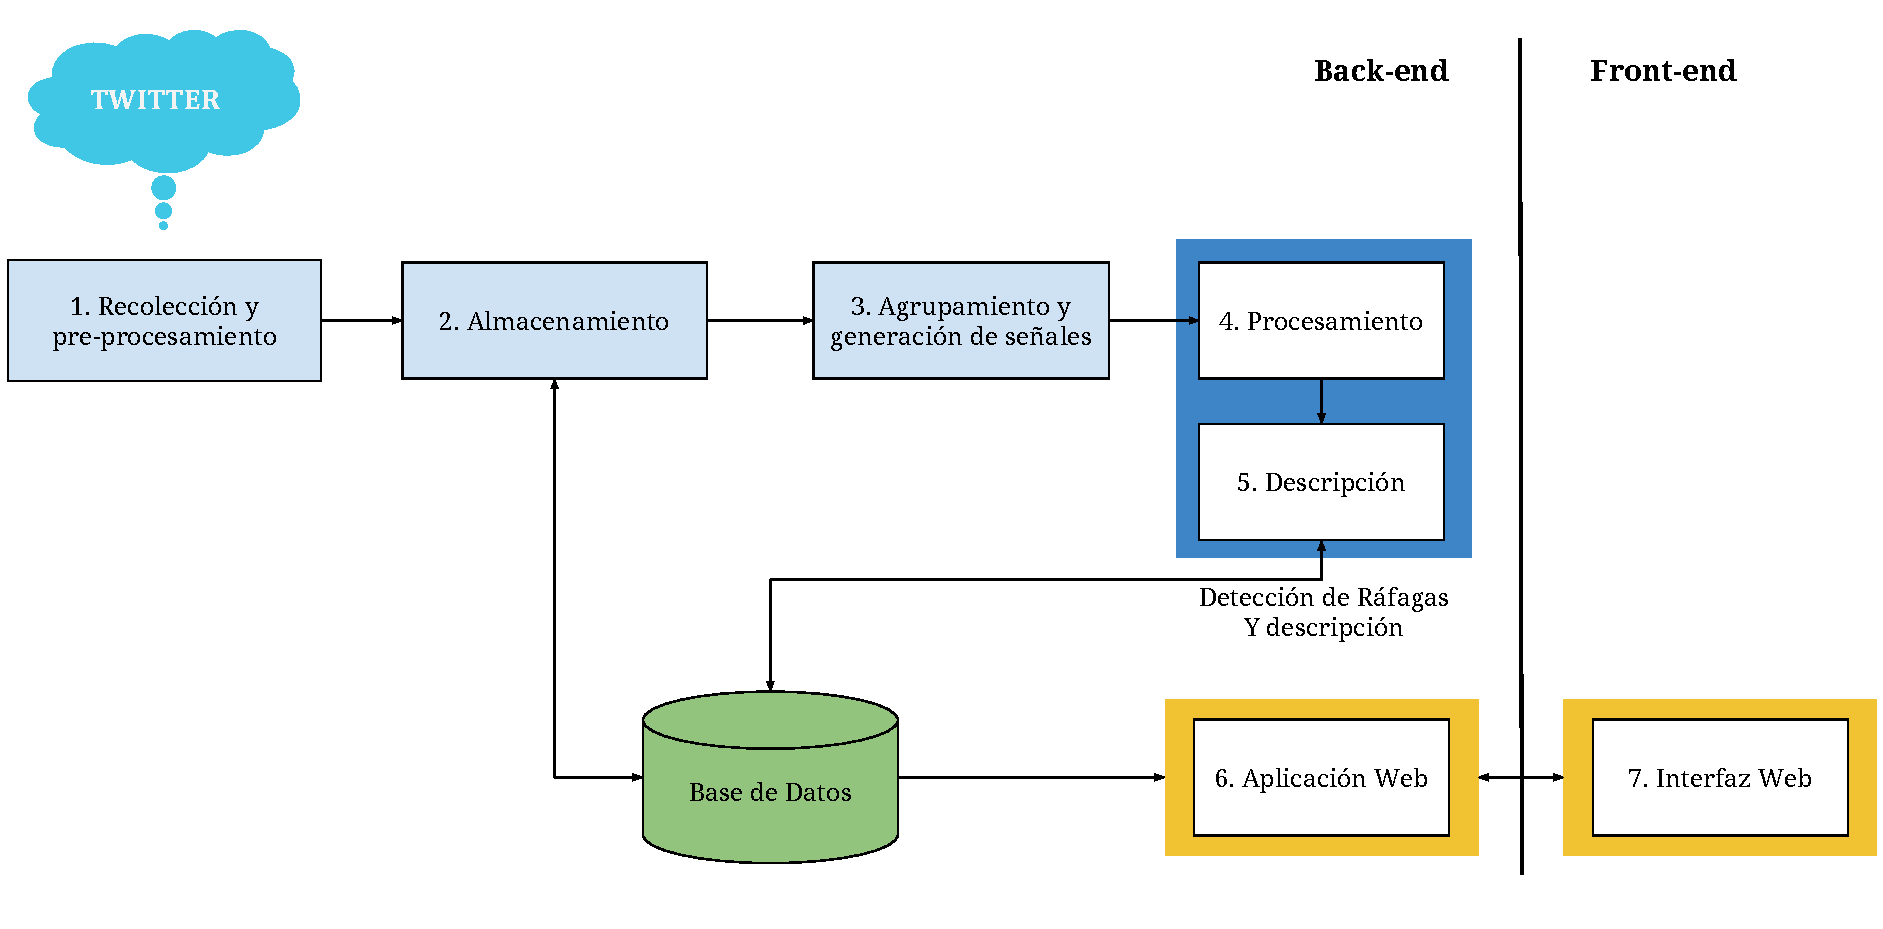
\includegraphics[width=\linewidth]{imagenes/Arquitectura.pdf}
	\caption{Arquitectura del sistema completo}
	\label{img:arquitectura}
\end{figure}

La figura \ref{img:arquitectura} es un esquema de los módulos que conforman el sistema y la forma en que cada uno interactúa con los demás. 
%
Cabe destacar que la experimentación fue una parte importante de este trabajo de tesis. Es por esto que algunos de los procesos generan información que fue evaluada durante la etapa de análisis y que, en base a los resultados obtenidos, no se incluyó en las visualizaciones. 
%
Sin embargo toda la información generada quedó almacenada de forma ordenada para investigaciones futuras. 


A continuación se explican en detalle la función de cada uno de los módulos y las herramientas utilizadas para su implementación: 


\noindent\textbf{1) Recolección de datos y pre-procesamiento}

El módulo 1 se encarga de recibir el flujo de \textit{tweets} a medida que estos son publicados en la red social. 
%
Para obtener los datos se utiliza la API para acceder al \textit{stream} público de Twitter\footnote{\url{https://dev.twitter.com/streaming/public}} y una librería en Java\footnote{\url{http://twitter4j.org/}} que integra el servicio con la aplicación.
%
Los datos se reciben en formato JSON\footnote{\url{https://dev.twitter.com/docs/tweet-entities}}.

Los \textit{tweets} recolectados reciben un primer procesamiento encargado de agregar metadatos a partir del texto y de otras características del \textit{tweet}. El pre-procesamiento de los datos incluye:
\begin{itemize}
\item La ejecución del algoritmo SentiStreigth\footnote{\url{http://sentistrength.wlv.ac.uk}} para calcular el sentimiento del mensaje.
\item La búsqueda de menciones de nombres de países en diferentes idiomas en el mensaje y en los campos que incluyen información de localidad del usuario.
\item Etiquetado de \textit{tweets} de carácter posiblemente malicioso o casos particulares que perturban el correcto funcionamiento de la detección. Se marcan los \textit{tweets} publicados por el mismo usuario en un lapso menor a 5 minutos y también \textit{tweets} publicados por usuarios incluidos en una lista negra. La lista negra existe para casos particulares en que se detecten usuarios cuyas publicaciones entorpezcan el correcto funcionamiento de la aplicación (como fue el caso de una cuenta mexicana que todos los días publicaba la lista completa de sismos del día anterior). Esta lista puede ser actualizada sin necesidad de interrumpir los procesos. 
\end{itemize}

Los metadatos añadidos fueron parte importante del análisis experimental desarrollado. Se detalla un poco más sobre el proceso de extracción de sentimiento en la sección \ref{sec:sentimiento} y sobre el proceso de geolocalización en la sección \ref{sec:geocodificacion}. Además en el capítulo \ref{cap:analisis} se explica cómo se utilizaron estos datos en el análisis experimental y los resultados obtenidos.

Finalmente, luego de procesar cada \textit{tweet}, este es encolado en memoria caché para ser utilizado por el módulo 2.

\noindent\textbf{2) Almacenamiento de datos}

\begin{figure}[ht]
	\centering
	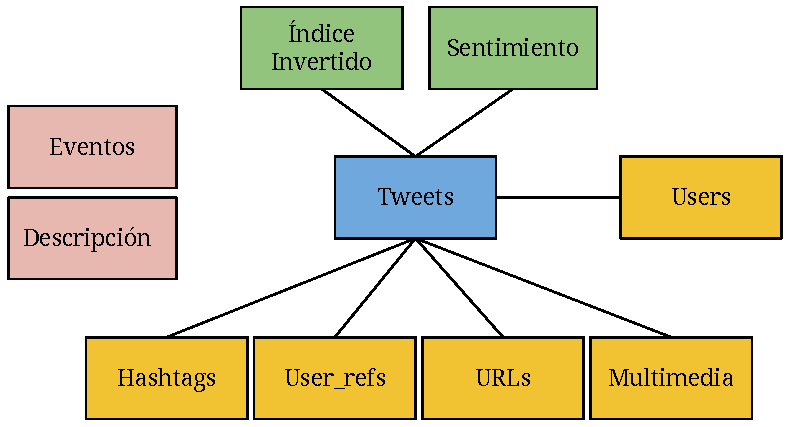
\includegraphics[width=0.8\linewidth]{imagenes/tweetmodel.pdf}
	\caption{Modelo de las tablas generadas diariamente que conforman la base de datos.}
	\label{img:database}
\end{figure}

El módulo 2 se encarga del almacenamiento de los \textit{tweets} recolectados y los metadatos asociados. La información se almacena en una base de datos relacional MySQL. 
%
Cada día se crean nuevas tablas para almacenar la información. Esta medida busca evitar tablas de gran tamaño y así optimizar los tiempos de búsqueda en la base de datos. 


La imagen \ref{img:database} muestra las tablas generadas diariamente. 
%
Las tablas de color amarillo almacenan información relacionada al \textit{tweet}. 
%
Los campos de estas tablas guardan información, en su mayoría, proveniente directamente desde Twitter.
%
Algunos de los datos almacenamos en estas tablas son generados en el módulo de pre-procesamiento, como la información de geolocalización y una etiqueta que indican si el \textit{tweet} fue publicado por un mismo usuario en un corto periodo de tiempo.
%
Las tablas de color verde almacenan otra información generada por el sistema.
%
Una de ellas almacena un índice invertido de las palabras que conforman el texto de los \textit{tweet} y la otra almacena el resultado del análisis de sentimiento para cada \textit{tweet}. 
%
Las tablas de color rosado almacenan la información relacionada con las detecciones y son pobladas con la información generada en los módulos 4 y 5 que se describen más adelante. 


Además de las tablas del modelo de la figura~\ref{img:database}, existen otras ``tablas virtuales'' o ``vistas'' destinadas al almacenamiento de datos agregados que son utilizados para la detección de ráfagas y para el almacenamiento de datos precalculados para las visualizaciones.
%
En el anexo \ref{anexo:database} se detalla el esquema de la base de datos y los campos que conforman cada tipo de tabla creada.

\noindent\textbf{3) Agrupamiento de \textit{tweets} y generación de señales}

El módulo 3 se encarga de preparar los datos para ser procesados en busca de ráfagas.
%
Los \textit{tweets} del \textit{stream} son agrupados en conjuntos etiquetados según el \textit{timestamp} de la fecha de creación. 
%
Cada conjunto de \textit{tweets} representa una ventana de tiempo individual. 
%
Las ventanas de tiempo son alineadas secuencialmente.
%
Cada secuencia de ventanas puede ser representada como una señal discreta, la que posteriormente es analizada en el módulo 4. 
%
Como parte de la experimentación se generaron diferentes tipos de señales a partir de algunos atributos de interés específicos. %Por ejemplo, señales conformadas por tweets que mencionaban un mismo país en el mensaje. 
%
Las señales a modo de experimentación fueron:

\begin{enumerate}
\item Señal de \textit{tweets} con palabras clave: Señal conformada por todos los \textit{tweets} que contienen cualquier palabra relacionada con sismos en cualquier idioma~\footnote{Palabras especificadas en una lista de palabras clave.}. 
\item Señales de localización del usuario: Señales construídas mediante la agrupación de tweets publicados por usuarios que indican pertenecer al mismo país en su perfil. Para esto se consideran los \textit{tweets} que contienen palabras relacionadas con sismos.
\item Señales de localización considerando el texto: Señales construídas mediante la agrupación de \textit{tweets} que mencionan el mismo país en el texto del mensaje. Para esto se consideran los \textit{tweets} que contienen palabras relacionadas con sismos.
\item Señales de idioma: Señales construídas mediante la agrupación de \textit{tweets} escritos en el mismo idioma. Para esto se consideran los \textit{tweets} que contienen palabras relacionadas con sismos.
\item Señales de sentimiento: Dos señales, una que agrupa los \textit{tweets} que reportan sismos y que expresan sentimiento positivo y otra con los \textit{tweets} que reportan sismos y que expresan sentimiento negativo. 
\end{enumerate}

Las diferentes señales creadas y los resultados obtenidos a partir de su análisis para detección de sismos se detallan en el capítulo\ref{cap:analisis}.

\noindent\textbf{4) Procesamiento}

El módulo 4 se encarga de procesar las secuencias de ventanas generadas por el módulo anterior y analizarlas en busca de ráfagas.  
%
Para analizar los datos se utiliza una estructura de datos de tabla de hash concurrente en donde se almacenan datos estadísticos asociados a cada ventana de tiempo. Esta estructura permite acceder a los datos en paralelo y mejorar el rendimiento.
%
En la sección \ref{sec:deteccion} se explica en más detalle el algoritmo utilizado para la detección de ráfagas.

\noindent\textbf{5) Descripción}

El módulo 5 se encarga de la descripción de eventos, es decir, se encarga de procesar la ventana de tiempo donde se detectó una ráfaga para determinar las palabras y los \textit{tweets} que propiciaron ese comportamiento.
%
Con esta información se complementa la información temporal y geográfica asociada a esa ventana de tiempo.
%
En conjunto toda esta información describe un evento, ya que responden a las preguntas sobre el cuándo, dónde y qué es lo que pasó específicamente en cada evento detectado.


\noindent\textbf{6) Aplicación Web}

El módulo 6 corresponde al servidor de la aplicación Web implementado en Python utilizando el \textit{framework} Flask\footnote{\url{http://flask.pocoo.org/}}. El servidor accede directamente a la base de datos y consulta los datos a medida que estos van siendo agregados. Para servir los datos en tiempo real se utiliza un caché con auto-refresco de 1 segundo, que evita sobrecargar el servidor cuando acceden muchas personas al mismo tiempo a la aplicación. 

\noindent\textbf{7) Interfaz}

El módulo 7 corresponde a la interfaz de la aplicación Web. Para su implementación se utilizaron las siguientes librerías:
\begin{itemize}
\item JQuery.js\footnote{\url{https://jquery.com/}}: Librería javascript para facilitar la manipulación de documentos y las llamadas Ajax. 
\item Bootstrap\footnote{\url{http://getbootstrap.com/}}: Framework para desarrollar aplicaciones responsivas y que funcionan en varios dispositivos.
\item D3.js\footnote{\url{https://d3js.org/}}: Librería javascript para manipular documentos basados en datos y generar visualizaciones interactivas. %
\item Leaflet.js\footnote{\url{http://leafletjs.com/}}: Librería javascript para visualizaciones interactivas usando mapas. 
\item Leaflet.heat\footnote{\url{https://github.com/Leaflet/Leaflet.heat}}: Un plugin que extiende Leaflet para crear mapas de calor. 
\item Leaflet.markercluster\footnote{\url{https://github.com/Leaflet/Leaflet.markercluster}}: Un plugin que extiende Leaflet para agrupar marcadores cercanos entre si y desplegarlos de forma interactiva. 
\end{itemize}

En la sección \ref{sec:visualizacion} se detallan las visualizaciones utilizadas para presentar los datos y en la sección \ref{sec:aplicacion} se muestran vistas completas de la aplicación y su modo de uso. 

\section{Recolección de Datos}
\label{sec:recoleccion}

Twitter tiene dos servicios para acceder a los datos públicos: 
%
La API de búsqueda, que permite realizar consultas usando palabras clave, idioma, coordenadas geográficas, etc. 
%
Y la API para acceder al \textit{stream} público y que permite obtener el flujo de \textit{tweets} publicados en tiempo real filtrado por palabras clave, idioma, etc.
%
La principal diferencia entre ambas son las limitaciones, ya que la API de búsqueda permite hacer una cantidad limitada de consultas por minuto y la API del \textit{stream} limita la muestra de datos entregada para que no exceda al 1\% del total de mensajes publicados en Twitter en ese momento.
% 
Para este caso, a diferencia de Sakaki et al.\cite{sakaki2013tweet}, Robinson et al. \cite{robinson2013sensitive} y Earle et al. \cite{earle2012twitter}, se decidió ocupar la API para acceder al \textit{stream} público, como también lo hacen Avennuti et. al \cite{avvenuti2014earthquake}.
%
Mediante el uso de la API para acceder al \textit{stream} es posible obtener los \textit{tweets} más rápido y detectar en tiempo más cercano al ``tiempo real''. %Además, los filtros que se utilizaron para obtener los datos disminuyen el número de \textit{tweets} y según nuestra apreciación, la limitante que impone Twitter sobre la muestra de los datos no alcanza a ser suficientemente ajustada como para evitar que se obtengan todos los \textit{tweets} de interés. 

\begin{wrapfigure}{r}{0.5\textwidth}
	\vspace{-20px}
  \centering
    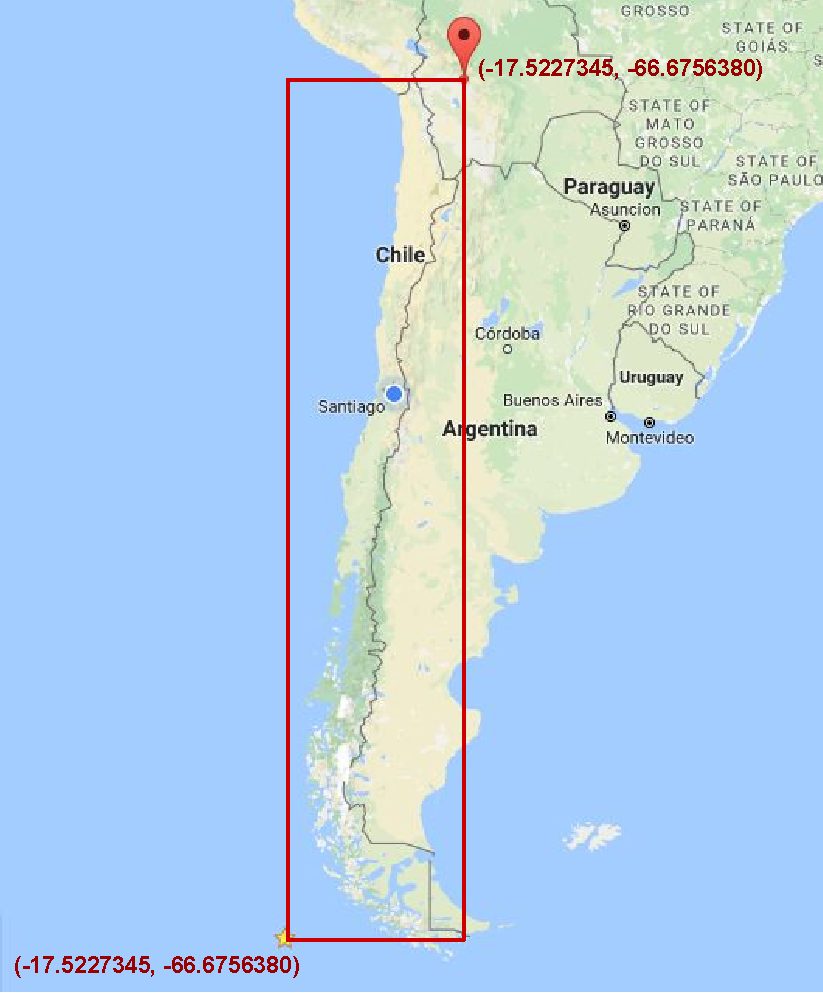
\includegraphics[width=0.48\textwidth]{imagenes/boundingbox.pdf}
  \caption{Cuadro de delimitación geográfica utilizado para recolectar \textit{tweets} de Chile.}
  \label{img:boundingbox}
  \vspace{-10px}
\end{wrapfigure}

Para obtener los datos, se filtró el flujo de mensajes para obtener todos los \textit{tweets} que mencionan alguna de las palabras clave relacionadas con eventos sísmicos. 
%
Las palabras clave corresponden a las traducciones de ``temblor'', ``sismo'' y ``terremoto'' en diferentes idiomas. 
%
La lista de palabras clave utilizadas es la siguiente: 
\jm{Agregar lista de palabras clave}
%
Además del filtro por palabras clave, se agrega un filtro (OR lógico) en forma de cuadro de límite geográfico que rodea todo el territorio nacional, tal como se muestra en la figura \ref{img:boundingbox}.
%
De esta forma se obtiene una muestra representativa de reportes de sismos en el mundo y de \textit{tweets} publicados por usuarios Chilenos geolocalizados que nos permiten mejorar la caracterización de sismos en Chile.


Los \textit{tweets} que conforman el flujo de Twitter no son descartados como en soluciones similares~\cite{avvenuti2014ears}. 
%
Esto significa que \textit{re-tweets} y \textit{tweets} que citan otros \textit{tweets} y que están relacionados con sismos o que se encuentran dentro del cuadro geográfico, son analizados junto con los originales. 
%
Esto hace que las señales a analizar sean más ruidosas, pero aumenta el volúmen del flujo de \textit{tweets}, lo que es útil para caracterizar mejor los eventos. 


El alcance mundial que se intenta cubrir trae consigo la dificultad de tener que procesar mensajes que están escritos en diferentes idiomas. 
%
Una tarea crucial para la detección y la descripción de cada evento es la de segmentar las oraciones en palabras.
%
Esta tarea es relativamente simple para casi todos los idiomas cuando se usan los elementos específicos de separación para cada uno (por ejemplo: espacios, puntos, comas, apóstrofes, etc.).
% 
Sin embargo, para idiomas que no utilizan signos de separación es complejo. 
%
Este es el caso del idioma chino, para el cual se utilizó la librería {\em Stanford NLP Chinese Word Segmentation}\footnote{\url{http://nlp.stanford.edu/projects/chinese-nlp.shtml}}.


Algunos usuarios o robots automáticos son utilizados para reportar periódicamente todos los últimos sismos ocurridos, por ejemplo, a lo largo del día previo. 
%
Al ser de carácter automático, estas publicaciones se hacen seguidas una de otra y en un corto periodo de tiempo. 
%
Este comportamiento puede, erróneamente, ser considerado como una ráfaga de reportes de sismos y ser reportado como una detección falsa.  
%
Usuarios con malas intenciones también pueden utilizar este mecanismo para difundir un rumor. 
%
Para evitar este problema, al momento de recolectar los tweets, se añade una \textit{etiqueta} a los tweets publicados por el mismo usuario en un periodo inferior a 5 minutos desde que publicó el mensaje previo, para luego no considerarlos en la detección. 
%
Si ocurre un sismo, se espera que éste sea reportado por varios usuarios en la misma ubicación geográfica, por lo que la detección no se verá afectada por este filtro. 


\section{Metodología de detección de sismos}
\label{sec:deteccion}

Uno de los objetivos específicos de esta tesis es proveer una metodología para detectar la ocurrencia de sismos. 
%
Con la finalidad de mejorar el trabajo realizado en estado del arte, se busca que la metodología propuesta permita detectar sismos en cualquier parte del mundo en tiempo cercano al tiempo real y que no dependa de procesos de clasificación supervisada de los mensajes (por lo tanto, que no tenga costos asociados al trabajo de etiquetado). 


El algoritmo utilizado para la detección de sismos es una adaptación de un enfoque no supervisado de detección de anomalías en flujos de texto presentado por Guzmán y Poblete~\cite{guzman2013line}. 
%
El algoritmo original permite detectar eventos emergentes al analizar el flujo genérico de mensajes publicados en Twitter de forma eficiente.  
%
Esta adaptación formaliza el algoritmo original para ser utilizado para monitorear 
%señales de tiempo discretas menos genéricas que son creadas a partir del flujo de mensajes de Twitter
flujos de mensajes menos genéricos que son creados a partir del flujo de mensajes de Twitter, en este caso en particular, un flujo de mensajes relacionados con sismos.
%
Se escogió este método porque tiene una complejidad lineal (en relación al número de mensajes de la entrada) y porque la configuración inicial es simple, requiriendo solamente el ajuste de algunos parámetros.
%
Mientras que otras técnicas de detección de eventos requieren ajustar periódicamente los parámetros~\cite{mathioudakis2010twittermonitor,sankaranarayanan2009twitterstand} o tienen complejidad computacional mayor, como las propuestas por Zhou et al.~\cite{zhou2015unsupervised} y Zhao et al.~\cite{zhao2014unsupervised} que tienen complejidad polinomial y cuadrática respectivamente. 


\subsection{Velocidad de Llegada Relativa}

El algoritmo original propuesto por Guzmán y Poblete se basa en comparar ventanas de tiempo consecutivas y detectar variaciones considerables entre la velocidad de llegada relativa calculada para las palabras que componen los mensajes en cada ventana de tiempo.

Para definir formalmente la velocidad de llegada relativa se considera ${\mathcal F} = \langle F_1, F_2, \dots, F_n \rangle$ un flujo de mensajes indexados por tiempo , donde  $t: {\mathcal F} \rightarrow \mathbb{R}^+$ indica el tiempo de llegada de los mensajes, $F_i \subseteq A$ es el conjunto de atributos del mensaje $F_i$ y $A$ es el conjunto de posibles atributos de los mensajes entre los que se encuentran las palabras clave, localidades, \textit{hashtags}, sentimiento inferido, entre otros.  

En el conjunto de posibles atributos en $A$ existen algunos que constituyen \emph{elementos de interés}, los cuales dependen de lo que se quiera detectar (en este caso, atributos que podrían estar relacionados con sismos) y que se denotan como $K \subseteq A$.

Además se denotan:
\begin{itemize}
	\item $w_i = \langle w^s_i, w^e_i \rangle$ como una ventana de tiempo que abarca desde el tiempo $w^s_i$ hasta el tiempo $w^e_i$.
 	\item $M_i = \{ s \in {\mathcal F}: w^s_i \le t(s) \le w^e_i \}$ como el conjunto de los mensajes de ${\mathcal F}$ dentro de la ventana de tiempo. 
	\item $\operatorname{freq}(K, M_i) = | \{ F \in M_i: K \cap F \neq \emptyset \} |$ como cantidad de mensajes dentro $M_i$ que contienen elementos de interés.
\end{itemize}

Finalmente, en el método propuesto, el flujo de datos es procesado en grupos, dividiendo los mensajes que llegan en ventanas de tiempo consecutivas de largo fijo $T$.

Considerando todo lo anterior, para una ventana de tiempo dada $w_i$ que contiene los mensajes $M_i$, se define la \emph{velocidad de llegada relativa} ($\lambda$) de elementos de interés en esta ventana como:

\begin{equation}
\label{eq:lambda}
\lambda(K, M_i) = \frac{\mathrm{freq}(K,M_i)}{T|M_i|}
\end{equation}

\subsection{Adaptación de la metodología de detección}

\begin{wrapfigure}{r}{0.5\textwidth}
	\centering
	\vspace{-30px}
	\subfloat[a][Distribución de la frecuencia de los mensajes relacionados con sismos 
		en ventanas de tiempo de 300 segundos.]{
		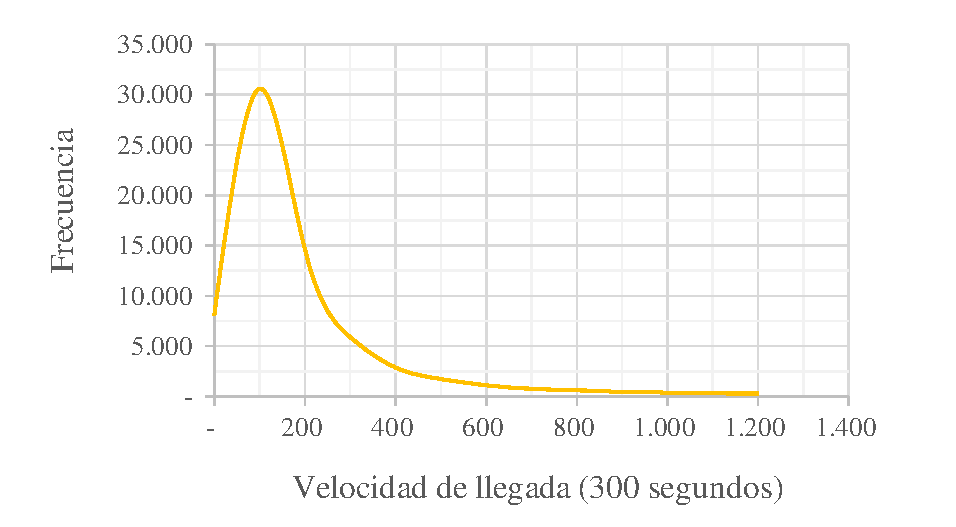
\includegraphics[trim={20 6 0 6}, clip, height=140pt]{imagenes/distribucion_02.pdf}
		\label{fig:data_distribution1}
	}\par\medskip
	\subfloat[b][Distribución del logaritmo de la frecuencia de los mensajes relacionados 
  		con sismos en ventanas de tiempo de 300 segundos.]{
  		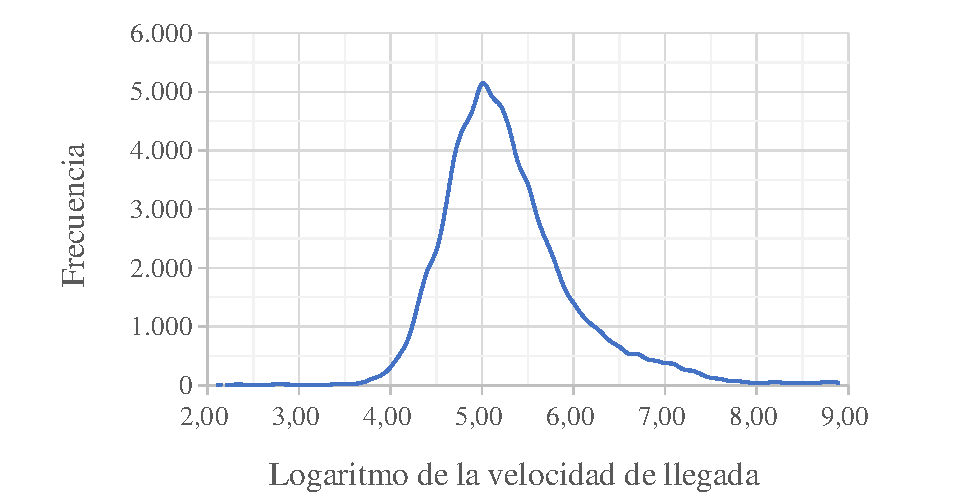
\includegraphics[trim={20 0 0 0}, clip, height=140pt]{imagenes/distribucion_03.pdf}
  		\label{fig:data_distribution2}
  	}
\end{wrapfigure}

La metodología propuesta se basa en monitorear el flujo de mensajes ($\mathcal{F}$) en el tiempo, para determinar cuándo una variación positiva en la velocidad de llegada relativa ($\lambda$) de elementos de interés es significativamente más grande que otras variaciones producidas por el ruido observado en el pasado.
%
Originalmente, en el método propuesto por Guzman y Poblete, la ``explosividad'' de cada palabra es estimada en base a la magnitud del cambio de su velocidad de llegada relativa ($\lambda$) con respecto a la ventana de tiempo previa.
%
La salida es una lista de los top-\emph{k} términos ordenados en orden decreciente según el cambio de su velocidad de llegada relativa ($\lambda$).
%
Esto no es suficiente para el propósito de la detección de sismos, ya que, como se detalló en la sección \ref{sec:recoleccion}, los datos que conforman el flujo fueron seleccionados a partir de palabras clave y datos geográficos. 
%
Ocasionando que, para este caso particular, se requiera monitorear un flujo sesgado en el que hay pocas palabras muy frecuentemente usadas (menos de \emph{k} palabras) y que experimentan pequeños cambios en cada ventana de tiempo debido a fluctuaciones al azar en los datos de entrada (i.e., ruido).
%
Por lo tanto, si se reportan las top-\emph{k} palabras más ``explosivas'' podría significar tener reportes en cada ventana de tiempo.
%
Es por esto, que para reportar sismos automáticamente se necesita estimar, de forma confiable, cuándo un cambio es significativo y por tanto indica actividad inusual.


El enfoque natural para determinar si la velocidad de llegada relativa ($\lambda$) experimenta una variación significativa durante una ventana de tiempo $w_i$ es monitorear la desviación estándar de $\lambda$ para todas las ventanas de tiempo hasta $w_{i-1}$; al igual que como se ha hecho en el trabajo previo sobre detección de eventos emergentes usando enfoques estadísticos basados en la distribución de frecuencias~\cite{kleinberg2003bursty, mathioudakis2010twittermonitor,
nguyen2013event}.
%
Esta idea asume y requiere que la velocidad de llegada relativa ($\lambda$) tenga una distribución exponencial. 
%
Sin embargo, un análisis empírico cuyo resultado se muestra en la figura ~\ref{fig:data_distribution1}, usando el conjunto de datos recolectados durante un periodo de 9 meses, desde el 25 de Enero al 25 de Octubre del 2016, indica que esto no se cumple para el caso de la distribución de la velocidad de llegada de las palabras relacionadas con sismos.
%
Esta observación hizo necesario un análisis para identificar como adaptar el algoritmo a los propósitos descritos en esta tesis.


Entre los análisis realizados hay uno en particular que resultó útil para continuar. Se aplicó una transformación logarítmica a los datos, tal como se muestra en la figura~\ref{fig:data_distribution2}, después de lo cual los datos se asemejan a una distribución {\em log-normal}.
%
Por lo tanto, en vez de monitorear los cambios en la velocidad relativa de llegada ($\lambda$), se modeló la distribución como si fuera {\em log-normal} y se monitorean los cambios en el logaritmo de la función. La función transformada se define como:

\begin{equation}
\label{eq:log_lambda}
\tilde{\lambda}(K, M_i) = \frac{\ln\left(\mathrm{freq}(K,M_i)\right)}{T |M_i|}
\end{equation}

Usando la función transformada $\tilde{\lambda}(K, M_i)$ se calculó su {\em z}-score\footnote{El z-score (standard score) indica a cuántas desviaciones estándar se encuentra un elemento de la media}. Este valor es monitoreado para identificar las variaciones significativas.  

\newcommand{\zscore}{\ensuremath{z\textnormal{-}\mathrm{score}}}
\begin{equation}
\label{eq:zscore}
\zscore(K, M_i) = \frac{\tilde{\lambda}(K, M_i)-\mu_i}{\sigma_i}
\end{equation}

\noindent donde $\mu_i$ y $\sigma_i$ son, respectivamente, el promedio y la desviación estándar de los valores observados de $\tilde\lambda$ durante las ventanas de tiempo $w_1, w_2, \dots, w_{i-1}$.

El método propuesto monitorea la señal discreta formada por los valores del {\em z}-score calculado para cada ventana de tiempo y catalóga como una detección de sismo cada uno de los instantes en donde $\zscore(K, M_i)\ge\theta$, donde $theta$ es un umbral definido experimentalmente.
%
En el capítulo~\ref{cap:analisis} se describen los experimentos realizados para determinar los parámetros iniciales y el valor del umbral para $\theta$. 
	
%\subsection{Metodología para ajustar los parámetros iniciales óptimos}
%
%La metodología de detección de sismos propuesta requiere que se fijen 3 parámetros iniciales:
%\begin{enumerate}
%\item El umbral para lanzar las alertas de detección de sismos $\theta$.
%\item La lista de atributos que definen un elemento de interés ($K$).
%\item El tamaño de cada ventana de tiempo ($T$).
%\end{enumerate}
%
%\medskip
%\noindent\textbf{(1) Umbral para detección de sismos ($\theta$):}
%%
%Para determinar las variaciones significativas en el flujo $\mathcal{F}$ se identificó el valor óptimo para el umbral $\theta$ empíricamente. 
%%
%Utilizando una muestra de datos de 2 meses, se probó el sistema de detección usando diferentes valores de $\theta$ y se seleccionó el valor que maximiza el F-measure.
%%
%La tabla~\ref{table:zscore} muestra los resultados obtenidos y el valor seleccionado $\theta=1.5$.
%\begin{table}
\centering
\begin{tabular}{cccc}
\toprule
{z-score ($\theta$)} & {Precision} & {Recall} & {F-Measure} \\ 
\midrule
{0.5}    & {48.1\%}     & {79.9\%}  & {60.1\%}  \\ 
{1.0}    & {62.6\%}     & {65.0\%}  & {63.8\%}  \\ 
{\bf 1.5}    & {\bf 88.3\%}     & {\bf 54.2\%}  & {\bf 67.1\%}  \\
{2.0}    & {92.3\%}     & {29.0\%}  & {44.2\%}  \\ 
\bottomrule
\end{tabular}
\caption{Comportamiento del algoritmo utilizando diferentes valores para el umbral de detecci\'on de sismos $\theta$.}
\label{table:zscore}
\end{table}

%
%
%\noindent\textbf{(2) Palabras clave relacionadas con sismos ($K$):} 
%Como se mencionó previamente, en esta adaptación los elementos de interés ($K$) son una lista de palabras clave relacionadas con la ocurrencia de sismos.
%%
%En esta tesis se extendió la lista de palabras entregada por investigadores del USGS, que fue usada en Earle et al.~\cite{earle2012twitter} y Avvenuti et al.~\cite{avvenuti2014earthquake,avvenuti2014ears}.
%%
%Sin embargo, a diferencia de los sistemas anteriores, la lista de palabras utilizada se construyó intentando incluir la mayor cantidad posible de palabras relacionadas con ocurrencias de sismos en cualquier idioma, incluso si incluía términos ambiguos (es decir, términos que a veces son utilizados en otros contextos).
%%
%Los mensajes ruidosos que puedan ser obtenidos al usar términos ambiguos no afectan el rendimiento de este método ya que es tolerante al ruido. 
%%
%Por ejemplo, la palabra ``quake'' puede ser usada para referirse a un videojuego o al personaje de un comic con el mismo nombre, o la palabra ``terremoto'' que en Chile también es utilizada para referirse a una bebida alcohólica típica y muy consumida durante las celebraciones nacionales. 
%%
%La lista de palabras está compuesta por los siguientes términos %{\em earthquake, sismo, quake, temblor, temblando, gempa, lindol, tremblement, erdbeben, deprem, seismós, séisme, zelzele, terremoto, scossa, bhukamp(sanskrit), \begin{CJK}{UTF8}{gbsn} 地震, 海啸, 津波, 地震, \end{CJK} \foreignlanguage{russian}{землетрясение}, \foreignlanguage{farsi}{زمین‌لرزه,زلزله}, \foreignlanguage{greek}{σεισμός}}
%%
%\jm{Agregar lista de palabras - Solucionar problema de codificación}
%Si se necesita agregar nuevos términos, la lista palabras puede ser actualizada dinámicamente.
%
%
%Además de las palabras clave relacionadas con sismos, se realizaron experimentos en los cuales además de las palabras clave, también se consideraban otros atributos para determinar si un elemento era de interés o no. 
%%
%De esta forma se pudo analizar la señal discreta asociada a diferentes tipos de atributos y determinar si estos agregaban valor a la detección o no. 
%%
%Entre estos atributos se encuentran:
%\begin{itemize}
%\item Sentimiento positivo del \textit{tweet}.
%\item Sentimiento negativo del \textit{tweet}.
%\item Idioma en el cual fue escrito el \textit{tweet}
%\item País mencionado en el texto del \textit{tweet}.
%\item País mencionado en la localidad de perfil del usuario que escribió el \textit{tweet}.
%\end{itemize}
%
%\begin{figure}[ht]
%  \centering
%  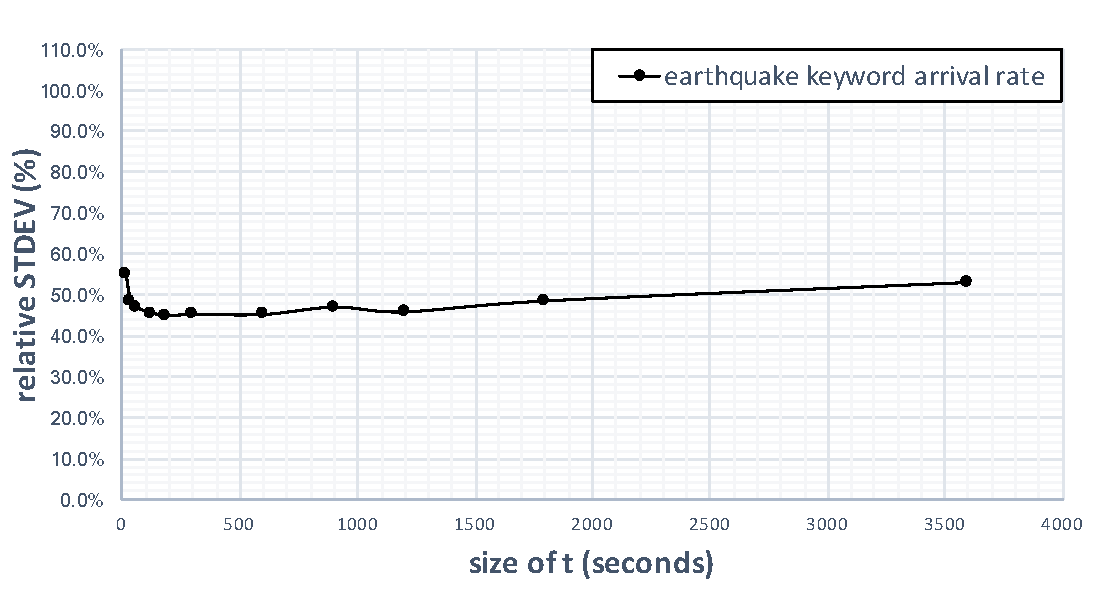
\includegraphics[trim={5 0 5 10}, clip, width=\textwidth]{imagenes/02_Poise_Analysis_WindowSize_solo.pdf}
%  \caption{Desviación estándar relativa de la señal que considera las palabras clave relacionadas con sismos para diferentes tamaños de ventana de tiempo (en segundos)}
%\label{fig:window_size}
%\end{figure}
%
%\noindent\textbf{(3) Tamaño de la ventana de tiempo ($T$):} 
%El tamaño de la ventana corresponde al largo del tiempo (en segundos) de cada conjunto de \textit{tweets} en los cuales son divididos los datos de la entrada para ser procesados por el algoritmo.
%%
%Este parámetro se determina analizando el flujo de la entrada y seleccionando un valor para $T$ que minimiza la desviación estándar relativa, es decir, cuando la frecuencia de aparición es más estable. 
%%
%Intuitivamente, si la ventana de tiempo es muy pequeña, los mensajes que contengan elementos en $K$ estarán distribuidos de forma más aleatoria en cada ventana. Esto significa que habrían ventanas de tiempo sin ninguna ocurrencia y otras con varias ocurrencias. Mientras más grande sea la ventana de tiempo, más factible es poder estimar la frecuencia en la ventana siguiente. 
%%
%Para determinar el valor de $T$ se utilizó el siguiente procedimiento, descrito en~\cite{guzman2013line}:
%%
%Para el flujo de entrada dado, se calcula la velocidad de llegada relativa de ventanas sucesivas $w_i$ de tamaño $T$.
%%
%Se repite este proceso para diferentes tamaños de ventana $T$ en el rango de $0$ hasta $3\,600$ segundos (una hora) para un periodo de 2 meses y se selecciona el $T$ con la desviación estándar relativa más pequeña. En este caso el valor de tamaño de ventana que minimiza la desviación estándar corresponde a los valores para $T \geq 300$ segundos, tal como se muestra en la figura~\ref{fig:window_size}.
%%
%Además, para disminuir los tiempos de detección, el sistema ejecuta dos procesos paralelos idénticos desfasados en $150$ segundos uno del otro y con ello asegurar un tiempo de detección de máximo 5 minutos. 
%
%%
%%In this experiment we
%%consider different possible input signals: 1) messages that contain an
%%earthquake keyword, 2) messages that contain an earthquake keyword and that
%%express positive sentiment\footnote{We extract the sentiment polarity of
%%Twitter messages using the off-the-shelf classifier SentiStrength
%%\url{http://sentistrength.wlv.ac.uk/}}, and 3) messages that
%%contain an earthquake keyword and that express negative sentiment. In our
%%experiment over a 2-month data stream we determine that the optimal
%%window-size must be greater than $120$ seconds, point at which the relative
%%standard deviation becomes stable.

\section{Análisis de Sentimiento}
\label{sec:sentimiento}

Uno de los objetivos específicos de esta tesis es la extracción de información u otros metadatos que permitan caracterizar los eventos sísmicos. 
%
Entre la información que se puede extraer de un \textit{tweet} se encuentra el análisis de sentimiento.
%
En particular en esta tesis se ejecutó una tarea básica en análisis de sentimientos que consiste en clasificar la polaridad de un texto.
%
Esta información fue utilizada para ver si al considerarlo dentro de los atributos de interés $K$ y analizar la señal asociada, mejoraba la detección cuando ocurría un sismo. 
%
La información queda almacenada en caso de ser útil en estudios posteriores que busquen estimar la intensidad de un evento o hacer otra especie de análisis. 


Para clasificar la polaridad del \textit{tweet} se utilizó el algoritmo SentiStreigth\footnote{\url{http://sentistrength.wlv.ac.uk}} con sus diccionarios específicos para diferentes lenguajes. 
%
Además se modificó el diccionario español agregando palabras pertenecientes al español ``chileno'' con el objetivo de mejorar la exactitud de la categorización en español.  


Dentro del conjunto de palabras que se agregaron del idioma español ``chileno'' se encuentran algunas utilizadas frecuentemente cuando se reporta un sismo y que denotan sorpresa, miedo o rabia, como improperios chilenos u otras expresiones comunes.
%
Además se agregaron palabras que denotan aprobación, como por ejemplo \textit{``bacán''}.


\section{Geocodificación de los datos}
\label{sec:geocodificacion}

Al recolectar los datos utilizando la API de Twitter se obtiene información asociada a cada \textit{tweet}. 
%
Esta información, en algunos casos, incluye información geográfica, dependiendo si el usuario tiene activado o no los mecanismos de geolocalización del dispositivo desde el cual publicó el mensaje.
%
El porcentaje de usuarios de Twitter que tienen activada la opción de compartir las coordenadas geográficas es muy bajo (cercano al 2\%) y varía dependiendo de cada país. 
%
Sin embargo, existen otros datos asociados a un \textit{tweet} que nos permiten inferir una posible ubicación desde la cual se publica ese mensaje. 
%
Estos datos no son 100\% confiables ni precisos y tampoco están disponibles para todos los \textit{tweets}, pero sin duda aumentan el porcentaje de \textit{tweets} para los cuales podemos aproximar una localidad llegando hasta un 80\%.


Las formas en que se obtuvo información relacionada a la localidad de un \textit{tweet} son:

\begin{enumerate}
\item Coordenadas GPS: Disponibles cuando el usuario tiene activado el mecanismo de GPS en su dispositivo y activada la opción que permite compartir estos datos en la red social.

\item Twitter Places: Cuando un usuario de Twitter escribe un mensaje asociado a algún lugar y tiene activado el GPS (no necesariamente permitiendo compartir las coodenadas), por ejemplo: \textit{``Que buen rato con amigas en el Starbucks''}. El dispositivo le sugiere al usuario agregar el lugar a partir de una lista de lugares que Twitter ya tiene almacenados, para este caso podría ser ``Starbucks Coffee, Agustinas, Santiago Centro, Santiago, Chile''. Si la persona acepta la sugerencia, esa información quedará asociada al \textit{tweet} y al ser un lugar que existe dentro de las bases de datos de Twitter, la información es muy completa.

\item Localidad del perfil del usuario: Cada usuario tiene la posibilidad de personalizar su perfil de Twitter. Entre los datos del perfil se encuentra información sobre su localidad, sin embargo, el usuario puede completar esta información ingresando texto libre. Como resultado, los usuarios escriben los nombres de los lugares de diferentes formas, con diferentes grados de precisión y por supuesto, también hay muchos nombres de lugares inexistentes o textos que no indican realmente dónde vive el usuario. A pesar de esto, este campo es muy utilizado por los usuarios de Twitter y en general si corresponde a información sobre un lugar real. 

\item Localidades mencionadas en el texto del \textit{tweet}: Al estar analizando \textit{tweets} que reportan sobre sismos, muchos de los mensajes incluyen nombres de localidades. Al igual que en el caso anterior, esta información puede estar escrita de diversas formas y siempre existe la posibilidad de que no sea información real. %Sin embargo esta información está presente en muchos de los mensajes y bajo el amparo de la ley de los grandes números, en esta tesis esta información también es considerada al momento de caracterizar un evento. 

\end{enumerate} 

Para extraer la información que se indica en los puntos 3. y 4. es necesario encontrar menciones de localidades en el texto disponible en el campo de localidad del usuario y en el corpus del \textit{tweet}. 
%
Para esto se utiliza un listado de nombre de países y sus traducciones a diferentes idiomas y un listado de ciudades chilenas que permite obtener información más detallada sobre localidades dentro de Chile. 
%
Para encontrar las menciones se analiza el texto buscando ocurrencias de países en primer lugar. Si el texto no contiene información de ningún país y el \textit{tweet} está escrito en español, se buscan nombres de ciudades chilenas. De la misma forma, para el caso de los \textit{tweets} escritos en japonés, se buscan nombres de ciudades de japón. 
%
Esto se puede extender para otros países de los cuales se quiera obtener información más detallada. Pero en esta tesis se evitó porque las coincidencias entre nombres de ciudades de diferentes países puede causar problemas en los resultados obtenidos. 
%
No se utilizó algo más sofisticado para extraer nombres de localidades debido a que estos datos tienen que ser procesados en tiempo real y no ocasionar cuellos de botella que retrasen los tiempos de la detección de sismos.

	
Una vez obtenidos los nombres de localidades, para información que se indica en los puntos 2, 3 y 4, es necesario además agregar coordenadas geográficas.
%
Para los casos en que solo se tiene información del país se les asignaron coordenadas genéricas en un punto céntrico del territorio. 
%
Para los casos en que hay información de las ciudades, se asignaron las coordenadas de la ciudad respectiva. 


\section{Visualización de datos}
\label{sec:visualizacion}
	\subsection{Temporales}
	
	\begin{figure}[ht]
	  \centering
	  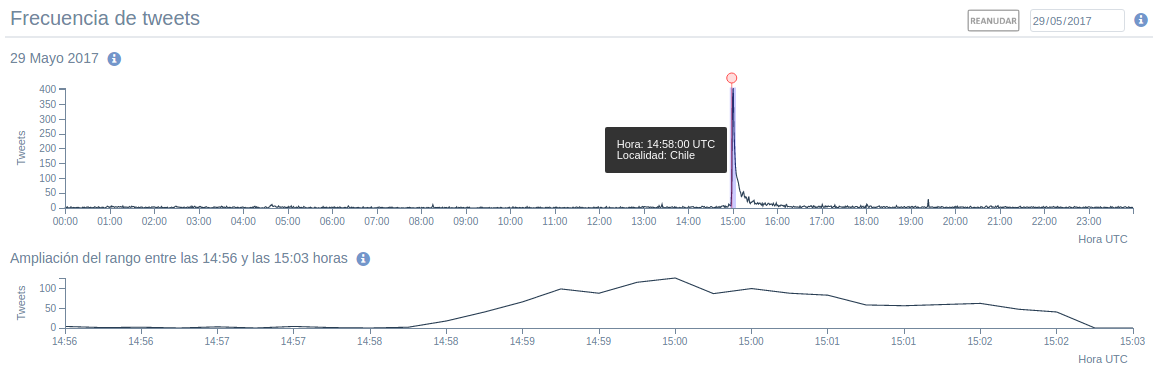
\includegraphics[trim={0 0 0 0}, clip, width=\textwidth]{imagenes/linea_de_tiempo_interactive.png}
	  \caption{Visualización de la frecuencia de \textit{tweets} de un día completo en intervalos de 60 segundos y de la frecuencia de \textit{tweets} de la zona seleccionada en intervalos de 15 segundos.}
	\label{fig:timeline}
	\end{figure}
		
	
	Para visualizar los datos temporales, se utiliza una señal interactiva similar a un gráfico de línea, que se actualiza a medida que pasa el tiempo y que muestra la cantidad de \textit{tweets} publicados en cada momento.
	%
	La imagen \ref{fig:timeline} corresponde a la visualización de los datos recolectados el día 29 de Mayo del 2017.
	%
	La primera señal muestra los datos recolectados en un rango de un día y la segunda señal muestra el rango seleccionado amplificado. Por defecto, están seleccionados los últimos 30 minutos.
		
	Mediante esta visualización es posible identificar rápidamente cambios en el comportamiento típico de los usuarios.
	%
	Además el sistema marca automáticamente los puntos de interés, en este caso, los puntos en donde inicia un sismo. 
	%
	Los usuarios pueden interactuar con esta visualización, ya sea seleccionando un rango de tiempo o haciendo \textit{click} en un punto de interés, lo que permite obtener información más detallada de el periodo de tiempo seleccionado. 
	
	
	\subsection{Geográficos}
	
	\begin{figure}[ht]
	\centering
	\subfloat[Mapa del mundo con \textit{tweets} geolocalizados.]{
		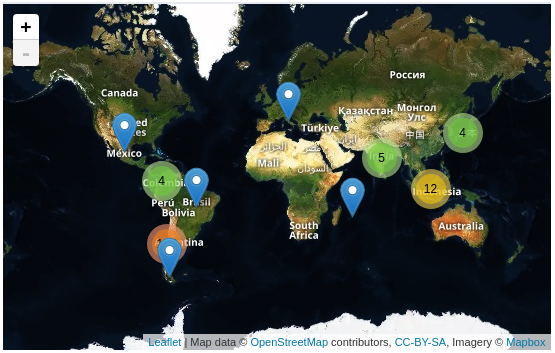
\includegraphics[height=140pt]{imagenes/worldmap.png}
		\label{fig:worldmap-out}
	}
	\hfill
	\subfloat[Mapa ampliado a la zona afectada por el sismo.]{
  		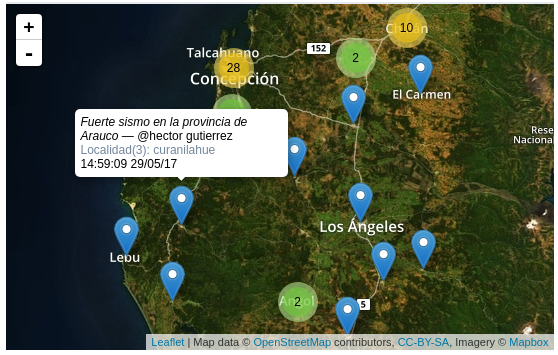
\includegraphics[height=140pt]{imagenes/worldmap-maxzoom.png}
  		\label{fig:worldmap-zoom}
  	}
  	\caption{Mapa interactivo con marcadores para cada tweet geolocalizado y agrupados en base a la distancia que existe entre ellos. Las imagenes corresponden a un sismo ocurrido cerca de  Concepción, Chile, el 29 de Mayo del 2017.}
  	\label{fig:worldmap}
  	\end{figure}
	 	
	  	
	Como se mencionó en la sección \ref{sec:geocodificacion} se intenta obtener la mayor cantidad posible de información geográfica. 
	%
	Esto es muy útil ya que, a pesar de no ser 100\% confiable, entrega una buena aproximación de la percepción de un sismo. 
	%
	Saber donde se encuentran los usuarios que reportan un sismo nos permite identificar las áreas afectadas y el alcance geográfico de cada evento. 
	%
	
	\begin{wrapfigure}{r}{0.4\textwidth}
	\vspace{-20px}
	  \centering
	  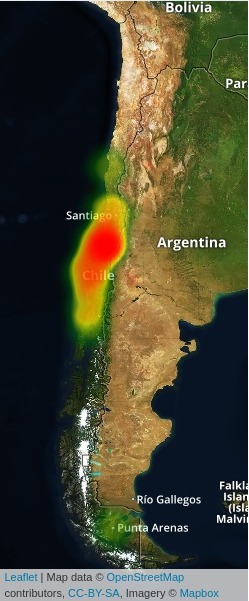
\includegraphics[trim={0 0 0 0}, clip, width=0.4\textwidth]{imagenes/heatmap.png}
	  \caption{Mapa de calor construido a partir de las coordenadas geográficas inferidas de los \textit{tweets} publicados durante un sismo en Concepción}
	\label{fig:heatmap}
	\vspace{-130px}
	\end{wrapfigure} 
	
	Para mostrar esta información se utilizan dos tipos de mapas, el primero consiste en un mapa de calor. 
	%
	La figura \ref{fig:heatmap} visualiza los datos recolectados durante los 15 minutos posteriores a un evento sísmico ocurrido el 29 de Mayo cerca de Concepción. 
	%
	En ella se puede observar la zona en donde se publicaron un mayor número de tweets y cómo esto se modifica en el tiempo.
	%
	%Como se puede observar, la imagen muestra una mancha roja un poco más abajo de Santiago. 
	%
	%Esto se debe a que este mapa no se encuentra normalizado. 
	%
	%Sin embargo el usuario tiene la opción de escoger ver el mapa normalizado por población regional, lo que permite observar más claramente que el evento ocurrió más al sur de Chile. 
	%
	%El mapa que muestra los mismos datos pero normalizados por región se muestra en la figura \ref{fig:heatmap-normalizado}.
	
	
	El segundo tipo de mapa consiste en un visualización interactiva del mapa del mundo con marcadores para cada tweet relacionado con alguna localización.
	%
	Para una mejor visualización, los datos se agrupan en base a su cercanía y se van separando en grupos más pequeños a medida que el usuario amplía el mapa o hace click en cada grupo. 
	%
	La figura \ref{fig:worldmap-out} muestra la visualización durante un sismo en Chile y la figura \ref{fig:worldmap-zoom} muestra el mismo instante pero con el mapa ampliado a la zona con mayor número de marcadores.
	%
	La visualización permite identificar rápidamente los lugares afectados, en este caso, en el mapa \ref{fig:worldmap-out} se identifica un grupo grande en Chile y a medida que se amplía esa zona, en el mapa \ref{fig:worldmap-zoom} se identifica un grupo numeroso en Concepción (ciudad muy cercana al epicentro) y las ciudades aledañas.
	
	
  	
\section{Aplicación Web}
\label{sec:aplicacion}

\subsection{Usuarios de la Aplicación}

Los usuarios finales de la aplicación son:

\begin{enumerate}
\item Sismólogos de las oficinas del Centro Sismológico Nacional de la Universidad de Chile (CSN)
\item Personas no expertas en sismología que deseen visitar el sitio Web
\end{enumerate}

\subsection{Diseño de la Aplicación}

El objetivo principal de la aplicación Web es presentar los datos a los usuarios expertos, es decir, a los sismólogos de las oficinas del CSN. 
%
La aplicación será visualizada en las pantallas de monitoreo ocupando pantallas ordenadas verticalmente, además se desea poder extraer la información relevante sin la necesidad de interacción.
%
Por otro lado, la aplicación que queda disponible para el resto de los usuarios debe ser fácil de comprender. 


Es de interés poder observar los datos en tiempo real y también se desea poder explorar la información de eventos pasados. 
%
Para cada evento se presenta información de geolocalización. 


Teniendo en cuenta los puntos antes mencionados se desarrollan dos vistas de la aplicación que presentan la misma información. 
% 
Las figuras \ref{fig:webapp} y \ref{fig:webapp_csn} muestran la vista de la aplicación disponible de manera pública y la utilizada por el CSN respectivamente. 
%
En ella se observan las visualizaciones descritas en la sección \ref{sec:visualizacion} y el listado de \textit{tweets}, que permite a los usuarios comprender mejor el evento. 

	\begin{figure}[ht]
	  \centering
	  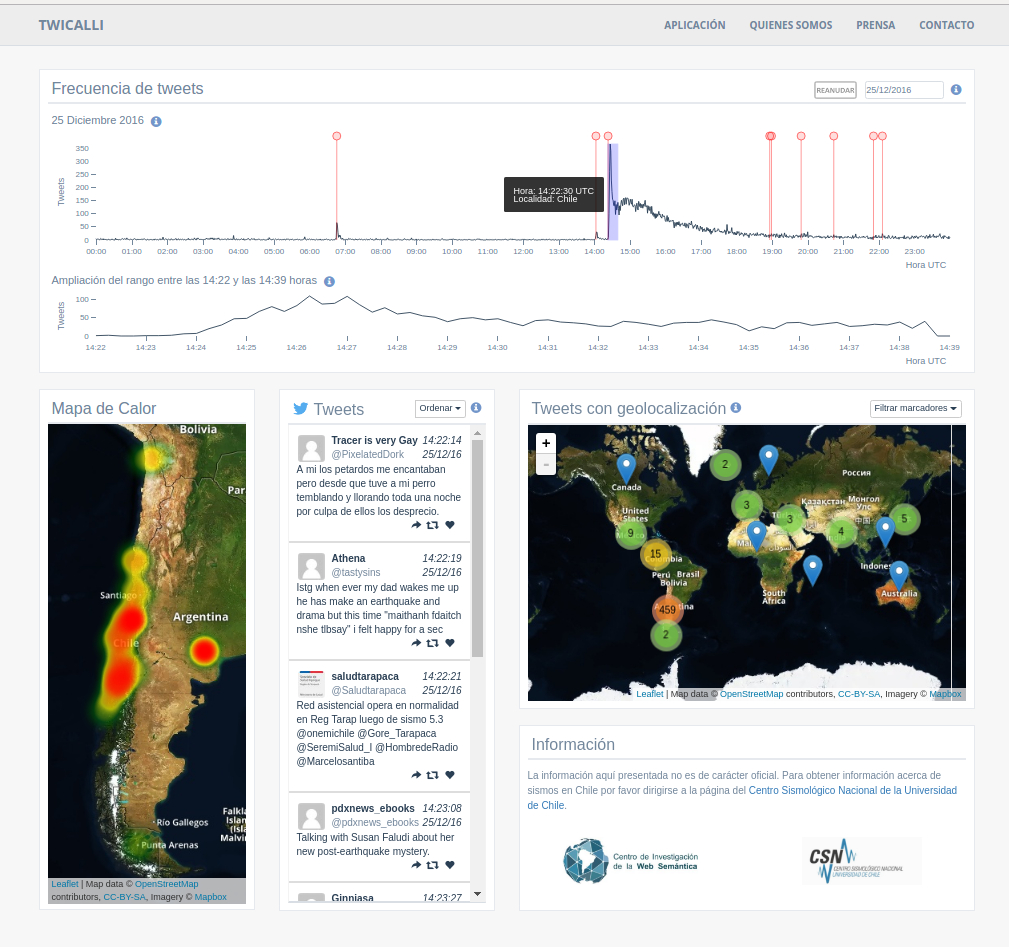
\includegraphics[trim={0 0 0 0}, clip, width=\textwidth]{imagenes/aplicacionexplorar.png}
	  \caption{Vista de la aplicación Web disponible públicamente}
	\label{fig:webapp}
	\end{figure}
	
	\begin{figure}[ht]
	  \centering
	  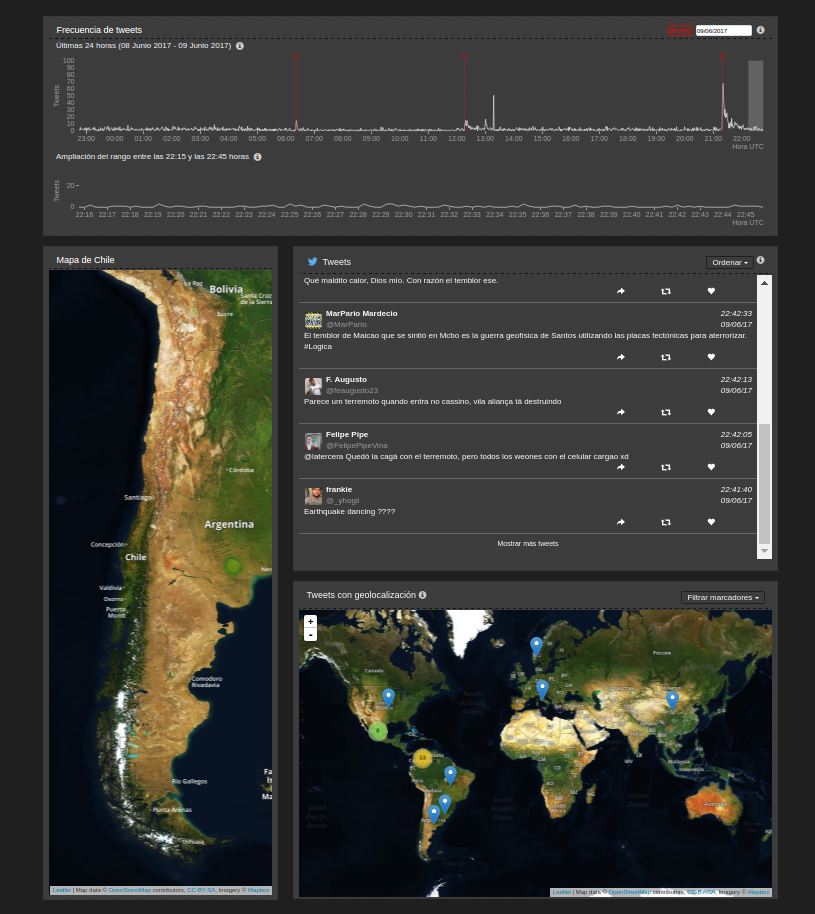
\includegraphics[trim={0 0 0 0}, clip, width=\textwidth]{imagenes/aplicacionexplorar_csn.png}
	  \caption{Vista de la aplicación Web utilizada por usuarios del CSN}
	\label{fig:webapp_csn}
	\end{figure}


Gracias a las iteraciones y la retroalimentación de los usuarios expertos se pudo identificar algunas mejoras, principalmente en la vista que visualizarán en las pantallas del CSN:

\begin{enumerate}
\item Preferencia por el uso de un mapa en el que se distinga el relieve del terreno y las fallas geográficas del borde costero chileno.
\item Selección de los colores utilizados en el mapa de calor y los marcadores para que no se confundan con los colores del mapa. 
\item Preferencia por el uso de una paleta de colores oscura para el fondo de la aplicación, debido a que el fondo blanco en las pantallas de monitoreo cansa la vista.
\end{enumerate}


\subsection{Interacciones}

La aplicación Web por defecto presenta los datos en tiempo real correspondiente a los últimos 30 minutos.
La línea de tiempo del día completo se actualiza cada 1 minuto y la línea de tiempo amplificada se actualiza cada 15 segundos. 
Además cada 1 segundo se consulta si hay nuevos \textit{tweets} y de ser así se dibujan en los mapas y en la parte superior de lista de tweets.  

Los usuarios pueden interactuar con la aplicación y en caso de hacerlo la actualización automática se detiene, pudiendo reanudarse en cualquier momento haciendo click en el botón \textit{reanudar} de la parte superior derecha de la línea de tiempo. 

Las interacciones disponibles son: 

\begin{itemize}
\item Seleccionar un largo de tiempo de la línea de tiempo principal. Esto permite actualizar la información en el resto de la página, mostrando el rango de tiempo amplificado y la información de los \textit{tweets} publicados durante ese rango de tiempo. 
\item Hacer click en un marcador rojo de la línea de tiempo principal, el cual representa la ocurrencia de un evento. Esta acción selecciona automáticamente el rango en el que aumentó el número de \textit{tweets} relacionados a ese evento y actualiza la información del resto de las visualizaciones de la misma forma que la interacción anterior. 
\item Hacer click en los marcadores del mapa que están agrupados para desagruparlos.
\item Hacer click en los marcadores desagrupados para mostrar información específica del \textit{tweet}.
\item Seleccionar una fecha para mostrar información de un día anterior. 
\end{itemize}




\chapter{Metodología de detección de sismos}
\label{cap:deteccion}

Uno de los objetivos específicos de esta tesis es proveer una metodología no supervisada para detectar la ocurrencia de sismos. 
%
Con la finalidad de mejorar el trabajo realizado en estado del arte, se busca que la metodología propuesta permita detectar sismos en cualquier parte del mundo en tiempo cercano al tiempo real y que no dependa de procesos de clasificación supervisada de los mensajes (por lo tanto, que no tenga costos asociados al trabajo de etiquetado). 


El algoritmo utilizado para la detección de sismos es una adaptación de un enfoque no supervisado de detección de anomalías en flujos de texto presentado por Guzmán y Poblete~\cite{guzman2013line}. 
%
El algoritmo original permite detectar eventos emergentes al analizar el flujo genérico de mensajes publicados en Twitter de forma eficiente.  
%
Esta adaptación formaliza el algoritmo original para ser utilizado para monitorizar 
%señales de tiempo discretas menos genéricas que son creadas a partir del flujo de mensajes de Twitter
flujos de mensajes menos genéricos que son creados a partir del flujo de mensajes de Twitter, en este caso en particular, un flujo de mensajes relacionados con sismos.
%
Se escogió este método porque tiene una complejidad lineal (en relación al número de mensajes de la entrada) y porque la configuración inicial es simple, requiriendo solamente el ajuste de algunos parámetros.
%
Mientras que otras técnicas de detección de eventos requieren ajustar periódicamente los parámetros~\cite{mathioudakis2010twittermonitor,sankaranarayanan2009twitterstand} o tienen complejidad computacional mayor, como las propuestas por Zhou et al.~\cite{zhou2015unsupervised} y Zhao et al.~\cite{zhao2014unsupervised} que tienen complejidad polinomial y cuadrática respectivamente. 

%\jm{Mencioné esto aquí, no sé si es suficiente o si lo pongo además como una nota al pie de página}
El trabajo descrito en este capítulo y la correspondiente evaluación descrita en el capítulo \ref{cap:analisis}, se realizó en colaboración con Jheser Guzmán como parte de su trabajo de doctorado.


\section{Velocidad de Llegada Relativa}

El algoritmo original propuesto por Guzmán y Poblete se basa en comparar ventanas de tiempo consecutivas y detectar variaciones considerables entre la velocidad de llegada relativa calculada para las palabras que componen los mensajes en cada ventana de tiempo.

Para definir formalmente la velocidad de llegada relativa se considera ${\mathcal F} = \langle F_1, F_2, \dots, F_n \rangle$ un flujo de mensajes indexados por tiempo , donde  $t: {\mathcal F} \rightarrow \mathbb{R}^+$ indica el tiempo de llegada de los mensajes, $F_i \subseteq A$ es el conjunto de atributos del mensaje $F_i$ y $A$ es el conjunto de posibles atributos de los mensajes entre los que se encuentran las palabras clave, localidades, \textit{hashtags}, sentimiento inferido, entre otros.  

En el conjunto de posibles atributos en $A$ existen algunos que constituyen \emph{elementos de interés}, los cuales dependen de lo que se quiera detectar (en este caso, atributos que podrían estar relacionados con sismos) y que se denotan como $K \subseteq A$.

Además se denotan:
\begin{itemize}
	\item $w_i = \langle w^s_i, w^e_i \rangle$ como una ventana de tiempo que abarca desde el tiempo $w^s_i$ hasta el tiempo $w^e_i$.
 	\item $M_i = \{ s \in {\mathcal F}: w^s_i \le t(s) \le w^e_i \}$ como el conjunto de los mensajes de ${\mathcal F}$ dentro de la ventana de tiempo. 
	\item $\operatorname{freq}(K, M_i) = | \{ F \in M_i: K \cap F \neq \emptyset \} |$ como cantidad de mensajes dentro $M_i$ que contienen elementos de interés.
\end{itemize}

Finalmente, en el método propuesto, el flujo de datos es procesado en grupos, dividiendo los mensajes que llegan en ventanas de tiempo consecutivas de largo fijo $T$.

Considerando todo lo anterior, para una ventana de tiempo dada $w_i$ que contiene los mensajes $M_i$, se define la \emph{velocidad de llegada relativa} ($\lambda$) de elementos de interés en esta ventana como:

\begin{equation}
\label{eq:lambda}
\lambda(K, M_i) = \frac{\mathrm{freq}(K,M_i)}{T|M_i|}
\end{equation}

\section{Adaptación de la metodología de detección}

La metodología propuesta se basa en monitorear el flujo de mensajes ($\mathcal{F}$) en el tiempo, para determinar cuándo una variación positiva en la velocidad de llegada relativa ($\lambda$) de elementos de interés es significativamente más grande que otras variaciones producidas por el ruido observado en el pasado.
%
Originalmente, en el método propuesto por Guzman y Poblete, la ``explosividad'' de cada palabra es estimada en base a la magnitud del cambio de su velocidad de llegada relativa ($\lambda$) con respecto a la ventana de tiempo previa.
%
La salida es una lista de los top-\emph{k} términos ordenados en orden decreciente según el cambio de su velocidad de llegada relativa ($\lambda$).
%
Esto no es suficiente para el propósito de la detección de sismos, ya que, como se detalló en la sección \ref{sec:recoleccion}, los datos que conforman el flujo fueron seleccionados a partir de palabras clave y datos geográficos. 
%
Ocasionando que, para este caso particular, se requiera monitorizar un flujo sesgado en el que hay pocas palabras muy frecuentemente usadas (menos de \emph{k} palabras) y que experimentan pequeños cambios en cada ventana de tiempo debido a fluctuaciones al azar en los datos de entrada (i.e., ruido).
%
Por lo tanto, si se reportan las top-\emph{k} palabras más ``explosivas'' podría significar tener reportes en cada ventana de tiempo.
%
Es por esto, que para reportar sismos automáticamente se necesita estimar, de forma confiable, cuándo un cambio es significativo y por tanto indica actividad inusual.

\begin{figure}[h]
\minipage{0.46\textwidth}
 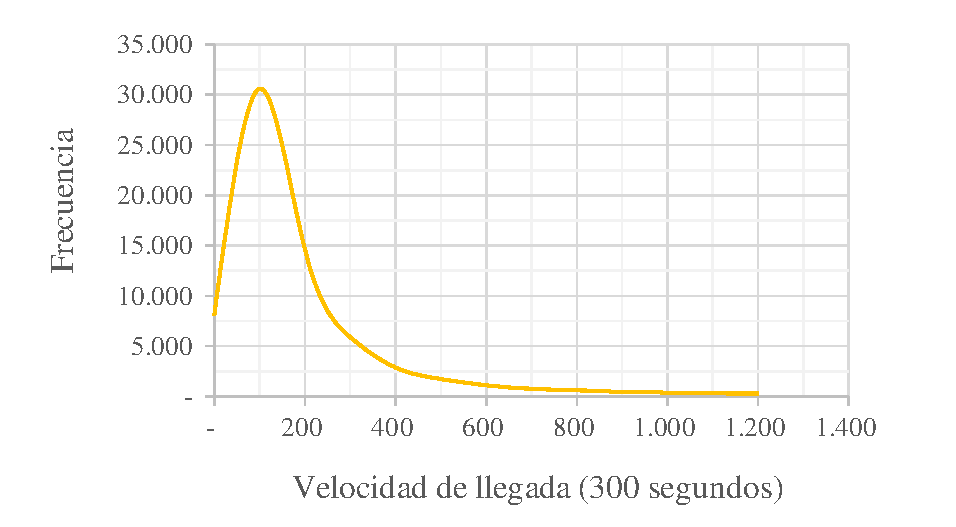
\includegraphics[trim={20 6 0 6}, clip, width=\linewidth]{imagenes/distribucion_02.pdf}
 \caption{Distribución de la frecuencia de los mensajes relacionados con sismos en ventanas de tiempo de 300 segundos.}
 \label{fig:data_distribution1}
\endminipage\hfill
\minipage{0.46\textwidth}
  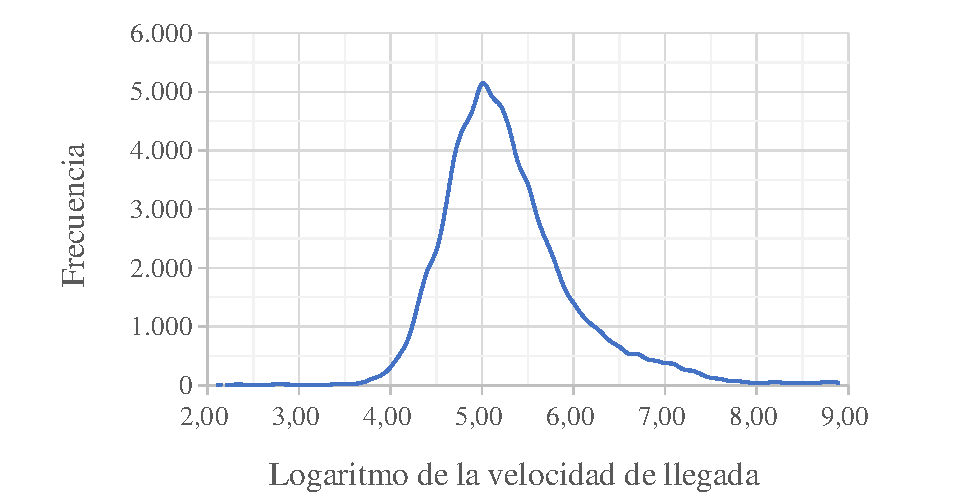
\includegraphics[trim={20 0 0 0}, clip, width=\linewidth]{imagenes/distribucion_03.pdf}
  \caption{Distribución del logaritmo de la frecuencia de los mensajes relacionados con sismos en ventanas de tiempo de 300 segundos.}
  \label{fig:data_distribution2}
\endminipage\hfill
\end{figure}


El enfoque natural para determinar si la velocidad de llegada relativa ($\lambda$) experimenta una variación significativa durante una ventana de tiempo $w_i$ es monitorizar la desviación estándar de $\lambda$ para todas las ventanas de tiempo hasta $w_{i-1}$; al igual que como se ha hecho en el trabajo previo sobre detección de eventos emergentes usando enfoques estadísticos basados en la distribución de frecuencias~\cite{kleinberg2003bursty, mathioudakis2010twittermonitor,
nguyen2013event}.
%
Esta idea asume y requiere que la velocidad de llegada relativa ($\lambda$) tenga una distribución exponencial. 
%
Sin embargo, un análisis empírico cuyo resultado se muestra en la figura ~\ref{fig:data_distribution1}, usando el conjunto de datos recolectados durante un periodo de 9 meses, desde el 25 de Enero al 25 de Octubre del 2016, indica que esto no se cumple para el caso de la distribución de la velocidad de llegada de las palabras relacionadas con sismos.
%
Esta observación hizo necesario un análisis para identificar como adaptar el algoritmo a los propósitos descritos en esta tesis.


Entre los análisis realizados hay uno en particular que resultó útil para continuar. Se aplicó una transformación logarítmica a los datos, tal como se muestra en la figura~\ref{fig:data_distribution2}, después de lo cual los datos se asemejan a una distribución {\em log-normal}.
%
Por lo tanto, en vez de monitorizar los cambios en la velocidad relativa de llegada ($\lambda$), se modeló la distribución como si fuera {\em log-normal} y se monitorizan los cambios en el logaritmo de la función. La función transformada se define como:

\begin{equation}
\label{eq:log_lambda}
\tilde{\lambda}(K, M_i) = \frac{\ln\left(\mathrm{freq}(K,M_i)\right)}{T |M_i|}
\end{equation}

Usando la función transformada $\tilde{\lambda}(K, M_i)$ se calculó su {\em z}-score\footnote{El z-score (standard score) indica a cuántas desviaciones estándar se encuentra un elemento de la media}. Este valor es monitorizado para identificar las variaciones significativas.  

\newcommand{\zscore}{\ensuremath{z\textnormal{-}\mathrm{score}}}
\begin{equation}
\label{eq:zscore}
\zscore(K, M_i) = \frac{\tilde{\lambda}(K, M_i)-\mu_i}{\sigma_i}
\end{equation}

\noindent donde $\mu_i$ y $\sigma_i$ son, respectivamente, el promedio y la desviación estándar de los valores observados de $\tilde\lambda$ durante las ventanas de tiempo $w_1, w_2, \dots, w_{i-1}$.

El método propuesto monitoriza la señal discreta formada por los valores del {\em z}-score calculado para cada ventana de tiempo y cataloga como una detección de sismo cada uno de los instantes en donde $\zscore(K, M_i)\ge\theta$, donde $theta$ es un umbral definido experimentalmente.
%
En el capítulo~\ref{cap:analisis} se describen los experimentos realizados para determinar los parámetros iniciales y el valor del umbral para $\theta$. 

\chapter{Enriquecimiento de la información}
\label{cap:procesamiento}

Uno de los objetivos específicos de esta tesis es la extracción de información u otros metadatos que permitan caracterizar los eventos sísmicos. 
%
La información del \textit{tweet} que se obtiene a partir de la API de Twitter contiene datos interesantes, tales como, el idioma en el que está escrito el mensaje y en algunos casos el lugar desde donde este fue publicado. Sin embargo, el porcentaje de mensajes con información geográfica asociada es muy bajo (2\%) y el idioma no es muy útil para inferir desde donde se publican los mensajes.
%
En conclusión, la información tal como es recibida no es suficiente para caracterizar los eventos. 

Lo que se consideró más relevante fue la obtención de datos geográficos, ya que etiquetar los mensajes en base al país de publicación es crítico si se desea detectar y monitorizar sismos de forma global.
Además, se espera poder dar un buen soporte especialmente para el caso de Chile, por lo que obtener información más granular respecto a la ubicación geográfica durante sismos en Chile también se considera importante. En la sección \ref{sec:geocodificacion} se detalla el trabajo realizado para enriquecer los datos geográficos asociados a los mensajes.

Con la intención de complementar la información con otros datos, se explora la posibilidad de analizar el sentimiento de los mensajes. La intuición tras esta decisión es observar si un cambio ``explosivo'' en el sentimiento general de los mensajes ayuda a detectar la ocurrencia de un evento sísmico. También abre posibilidades de trabajos futuros como, por ejemplo, el estudio de la correlación entre el sentimiento de los mensajes y la intensidad de un sismo. En la sección \ref{sec:sentimiento} se detalla la herramienta utilizada y cómo fue aplicada.

\section{Geocodificación de los datos}
\label{sec:geocodificacion}

Al recolectar los datos utilizando la API de Twitter se obtiene información asociada a cada \textit{tweet}. 
%
Esta información, en algunos casos, incluye información geográfica, dependiendo si el usuario tiene activado o no los mecanismos de geolocalización del dispositivo desde el cual publicó el mensaje.
%
El porcentaje de usuarios de Twitter que tienen activada la opción de compartir las coordenadas geográficas es muy bajo (cercano al 2\%) y varía dependiendo de cada país. 
%
Sin embargo, existen otros datos asociados a un \textit{tweet} que nos permiten inferir una posible ubicación desde la cual se publica ese mensaje. 
%
Estos datos no son 100\% confiables ni precisos y tampoco están disponibles para todos los \textit{tweets}, pero sin duda aumentan el porcentaje de \textit{tweets} para los cuales podemos aproximar una localidad, llegando hasta un 80\%.


Las formas en que se obtuvo información relacionada a la localidad de un \textit{tweet} son:

\begin{enumerate}
\item Coordenadas GPS: Disponibles cuando el usuario tiene activado el mecanismo de GPS en su dispositivo y activada la opción que permite compartir estos datos en la red social.

\item Twitter Places: Cuando un usuario de Twitter escribe un mensaje asociado a algún lugar y tiene activado el GPS (no necesariamente permitiendo compartir las coordenadas), por ejemplo: \textit{``Que buen rato con amigas en el Starbucks''}. El dispositivo le sugiere al usuario agregar el lugar a partir de una lista de lugares que Twitter ya tiene almacenados, para este caso podría ser ``Starbucks Coffee, Agustinas, Santiago Centro, Santiago, Chile''. Si la persona acepta la sugerencia, esa información quedará asociada al \textit{tweet} y al ser un lugar que existe dentro de las bases de datos de Twitter, la información es muy completa.

\item Localidad del perfil del usuario: Cada usuario tiene la posibilidad de personalizar su perfil de Twitter. Entre los datos del perfil se encuentra información sobre su localidad, sin embargo, el usuario puede completar esta información ingresando texto libre. Como resultado, los usuarios escriben los nombres de los lugares de diferentes formas, con diferentes grados de precisión y por supuesto, también hay muchos nombres de lugares inexistentes o textos que no indican realmente dónde vive el usuario. A pesar de esto, este campo es muy utilizado por los usuarios de Twitter y en general si contiene información sobre un lugar real. 

\item Localidades mencionadas en el texto del \textit{tweet}: Al estar analizando \textit{tweets} que reportan sobre sismos, muchos de los mensajes incluyen nombres de localidades. Al igual que en el caso anterior, esta información puede estar escrita de diversas formas y siempre existe la posibilidad de que no sea información real. %Sin embargo esta información está presente en muchos de los mensajes y bajo el amparo de la ley de los grandes números, en esta tesis esta información también es considerada al momento de caracterizar un evento. 

\end{enumerate} 

En los pocos casos de \textit{tweets} que contienen información GPS, la geolocalización es directa. 
%
Sin embargo, para los casos descritos en los puntos 2, 3 y 4, es necesario realizar procedimientos extra. 


Para extraer la información de localización que se indica en los puntos 3 y 4 es necesario encontrar menciones de localidades en el texto del campo de localidad del usuario y en el corpus del \textit{tweet}.  
%
Para esa tarea se utiliza un listado de nombres de países y sus traducciones a diferentes idiomas. 
%
Además, se cuenta con un listado de ciudades chilenas y de ciudades japonesas, que permite obtener información más detallada sobre localidades dentro de Chile y Japón, dos países altamente sísmicos y con un masivo uso de Twitter. 
%
Para encontrar las menciones se analiza el texto buscando ocurrencias de países en primer lugar, si el texto no contiene información de ningún país y el \textit{tweet} está escrito en español, se buscan nombres de ciudades chilenas. %De la misma forma, para el caso de los \textit{tweets} escritos en japonés, se buscan nombres de ciudades de japón. 
%
Esto se puede extender para otros países de los cuales se quiera obtener información más detallada. Pero en esta tesis se evitó, porque las coincidencias entre nombres de ciudades de diferentes países puede causar problemas en los resultados obtenidos. 
%
No se utilizó algo más sofisticado para extraer nombres de localidades debido a que estos datos tienen que ser procesados en tiempo real y no ocasionar cuellos de botella que retrasen los tiempos de la detección de sismos.

	
Una vez obtenidos los nombres de localidades para los casos 3 y 4, es necesario además agregar coordenadas geográficas.
%
Esto también aplica para el caso 2, en donde el \textit{tweet} tiene asociada información proveniente de \textit{Twitter Places}.
%
Para los casos en que solo se tiene información del país, se les asignaron coordenadas genéricas en un punto céntrico del territorio. 
%
Para los casos en que hay información de las ciudades, se asignaron las coordenadas de la ciudad respectiva. 


Un trabajo similar de inferencia de geolocalización al desarrollado en esta tesis fue utilizado en un estudio anterior sobre caracterización de eventos noticiosos chilenos en redes sociales \cite{maldonado2015spatio}. En ese estudio se complementa la información utilizando los lugares mencionados en el corpus de los mensajes que conforman cada evento y en la información del perfil de los usuarios que los emitieron, infiriendo los lugares donde ocurre cada evento y los lugares donde despertó interés la noticia respectivamente.

\section{Análisis de Sentimiento}
\label{sec:sentimiento}

%
El análisis de sentimiento, de forma general, se basa en la idea de utilizar técnicas de procesamiento de lenguaje natural, análisis de texto y lingüística computacional, para extraer, cuantificar y estudiar estados afectivos e información subjetiva. 
%
En particular en esta tesis se ejecutó una tarea básica en análisis de sentimientos que consiste en clasificar la polaridad de un texto, donde los polos son sentimiento positivo o sentimiento negativo. 


%La información obtenida fue utilizada a modo de experimentación y 
%
%En el análisis que se describe en el capítulo \ref{cap:analisis} se evaluó si al crear señales considerando la polaridad dentro de los atributos de interés $K$  mejoraba la detección al ocurrir un sismo. 
%
La información extraída mediante esta técnica se almacenó en una base de datos, quedando a disposición en caso de ser útil en estudios posteriores que busquen estimar la intensidad de un evento o hacer un análisis diferente. 


Para clasificar la polaridad del \textit{tweet} se utilizó el algoritmo SentiStreigth\footnote{\url{http://sentistrength.wlv.ac.uk}} en su versión para Java. 
%
Este algoritmo, el cual es de uso gratuito para fines de investigación, permite determinar la fuerza del sentimiento positivo o negativo en textos cortos, incluso si estos están escritos utilizando un lenguaje informal. 
%
SentiStrength reporta dos puntajes correspondientes a la fuerza del sentimiento:

\begin{center}
-1 (no negativo) a -5 (extremadamente negativo)\\
1 (no positivo) a 5 (extremadamente positivo)
\end{center}

Como se detalla en la documentación de la página Web de SentiStreigh, la razón por la que se reportan dos puntajes, es porque estudios sicológicos han demostrado que las personas procesan los sentimientos positivos y negativos en paralelo, como emociones mixtas.
%
Este algoritmo puede ser configurado para ser utilizado con textos en finlandés, alemán, holandés, español, ruso, portugués, francés, árabe, polaco, persa, sueco, griego, galés, italiano y turco. 
%
En los experimentos realizados, se utilizó con los idiomas disponibles, dejando fuera los mensajes escritos en idiomas como el Chino o el Japonés.


Con la finalidad de obtener una mejor adaptación del algoritmo al idioma español utilizado en Chile, se modificó el diccionario agregando palabras asociadas a modismos chilenos.
%
Dentro del conjunto de palabras que se agregaron se encuentran algunas utilizadas frecuentemente cuando se reporta un sismo y que denotan sorpresa, miedo o rabia, como improperios chilenos u otras expresiones comunes.
%
Además se agregaron palabras que denotan aprobación, como por ejemplo \textit{``bacán''}.

En el capítulo \ref{cap:analisis} se presentan los resultados obtenidos en la evaluación de las señales formadas a partir de la polaridad del sentimiento de los \textit{tweets}.




\chapter{Arquitectura del sistema}
\label{cap:arquitectura}

En este capítulo se describe la arquitectura del sistema desarrollado. El sistema completo tiene tres grandes  objetivos principales: la detección en tiempo real de sismos en Chile y en el mundo, la presentación de la información a los usuarios en tiempo real y el almacenamiento de datos históricos que permitan realizar otros estudios relacionados.

\begin{figure}[h]
	\centering
	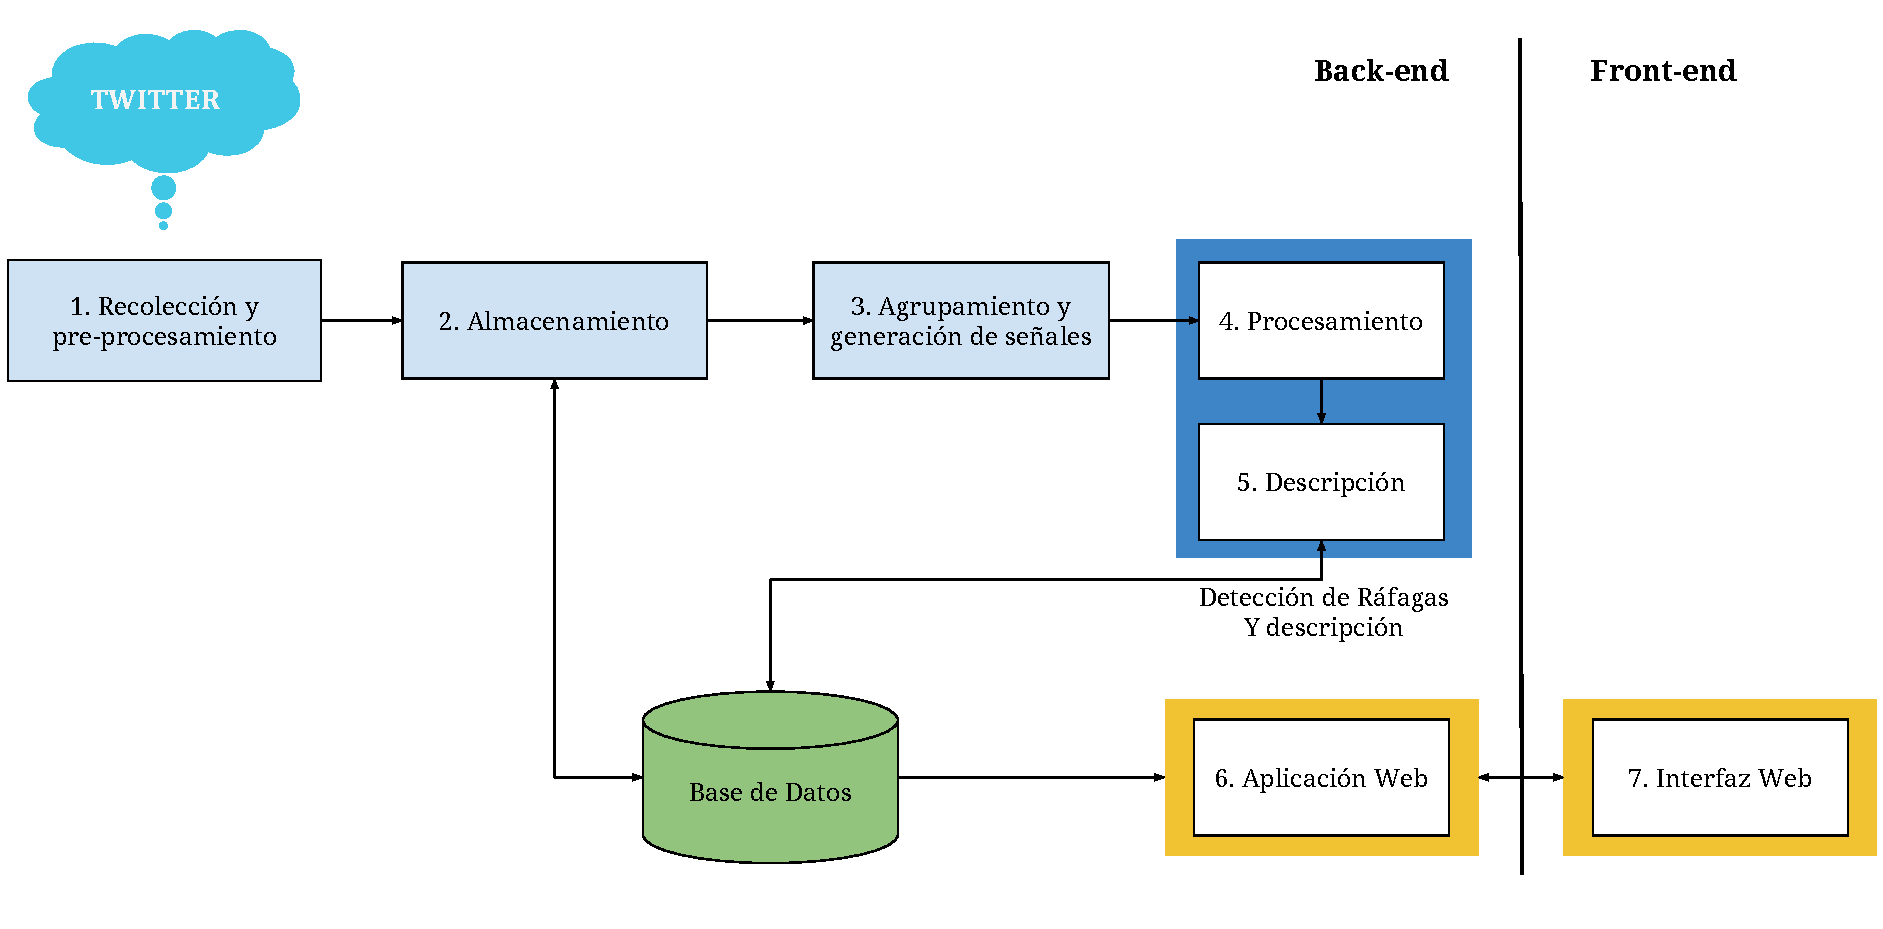
\includegraphics[width=\linewidth]{imagenes/Arquitectura.pdf}
	\caption{Arquitectura del sistema completo}
	\label{img:arquitectura}
\end{figure}

La figura \ref{img:arquitectura} es un esquema de los módulos que conforman el sistema y la forma en que cada uno interactúa con los demás. 
%
Cabe destacar que la experimentación fue una parte importante de este trabajo de tesis, es por esto que algunos de los procesos generan información que fue evaluada durante la etapa de análisis y que, en base a los resultados obtenidos, se tomó la decisión de no incluirla en las visualizaciones de la aplicación Web. 
%
Sin embargo, toda la información generada quedó almacenada en una base de datos en los servidores del Centro de Investigación de la Web Semántica para ser utilizada en investigaciones futuras. 

En las siguientes secciones se explica brevemente la función de cada módulo que compone el sistema.

\section{Recolección de datos y pre-procesamiento}
\label{sec:recoleccion}
El \textbf{módulo 1} se encarga de obtener el flujo de \textit{tweets} a medida que estos son publicados en la red social. Para esto se utiliza la API que provee Twitter para acceder a sus datos y algunos criterios de filtrado. 

\subsection{API de Twitter}

Twitter tiene dos servicios para acceder a los datos públicos: 
%
La API de búsqueda, que permite realizar consultas usando palabras clave, idioma, coordenadas geográficas, etc. 
%
Y la API para acceder al \textit{stream} público\footnote{\url{https://dev.twitter.com/streaming/public}} y que permite obtener el flujo de \textit{tweets} publicados en tiempo real filtrado por palabras clave, idioma, etc.
%
La principal diferencia entre ambas opciones son las limitaciones, ya que la API de búsqueda permite hacer una cantidad limitada de consultas por minuto y la API para acceder al \textit{stream} limita la muestra de datos entregada para que no exceda al 1\% del total de mensajes publicados en Twitter en ese momento.
% 
Para este caso, a diferencia de Sakaki et al.\cite{sakaki2013tweet}, Robinson et al. \cite{robinson2013sensitive} y Earle et al. \cite{earle2012twitter}, se decidió ocupar la API para acceder al \textit{stream} público, como también lo hacen Avennuti et. al \cite{avvenuti2014earthquake}.
%
Mediante el uso de la API para acceder al \textit{stream} es posible obtener los \textit{tweets} más rápido y detectar en tiempo más cercano al ``tiempo real''. Además, los filtros que se utilizan al obtener los datos disminuyen el número de \textit{tweets} de interés y según nuestra apreciación, la limitante que impone Twitter sobre la muestra de los datos no alcanza a ser suficientemente ajustada como para evitar que se obtengan todos los \textit{tweets} de interés. 

\begin{figure}[h]
	\centering
	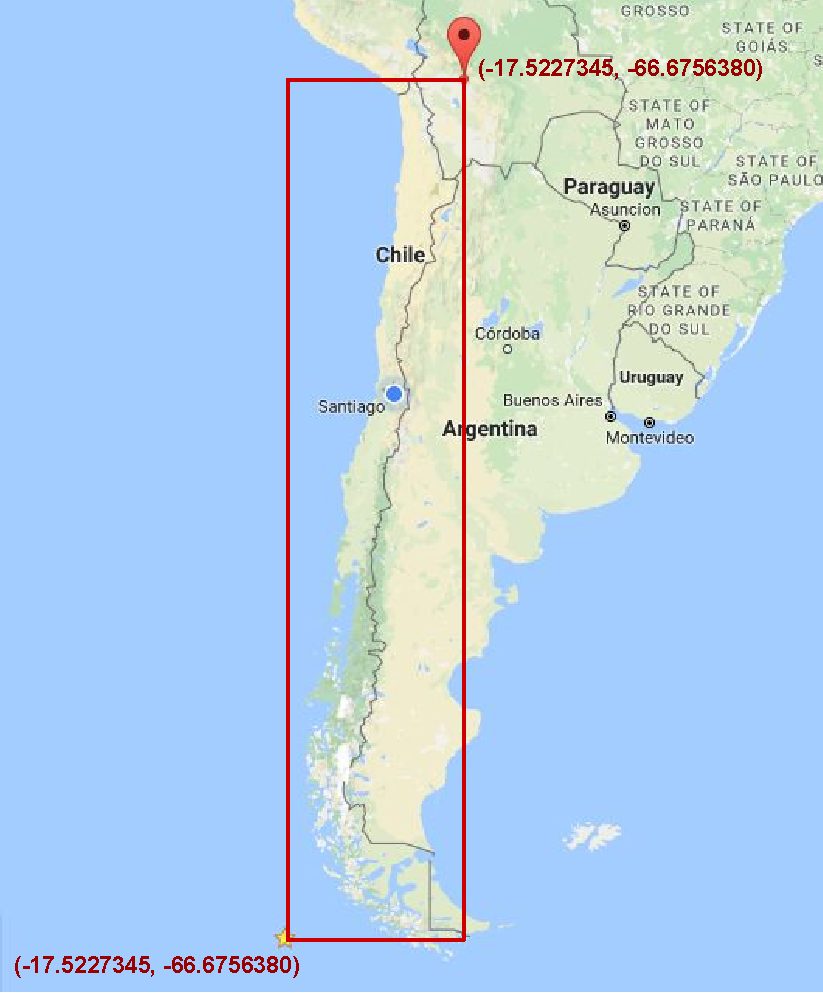
\includegraphics[width=0.5\linewidth]{imagenes/boundingbox.pdf}
	\caption{Cuadro de delimitación geográfica utilizado para complementar la recolección y obtener una mayor cantidad de información geolocalizada de Chile.}
	\label{img:boundingbox}
\end{figure}

\subsection{Criterios de selección de tweets}

Para obtener los datos, se filtró el flujo de mensajes para obtener todos los \textit{tweets} que mencionan alguna de las palabras clave relacionadas con eventos sísmicos. 
%
Las palabras clave corresponden a las traducciones de ``temblor'', ``sismo'' y ``terremoto'' en diferentes idiomas. 
%
La lista completa de palabras clave utilizadas se encuentran listadas en la figura \ref{img:keywords} en el capítulo \ref{cap:analisis}. 
%
Este criterio permite obtener \textit{tweets} provenientes de cualquier parte del mundo.

%
Además del filtro por palabras clave, se agrega un filtro (OR lógico) en forma de cuadro de límite geográfico que rodea todo el territorio nacional, tal como se muestra en la figura \ref{img:boundingbox}.
%
Con este criterio se obtiene una mayor cantidad de mensajes publicados por usuarios chilenos con información de geolocalización que permiten mejorar la caracterización de sismos en Chile.
%
Este filtro se puede modificar o extender para incluir otras áreas geográficas que requieran mayor atención, por ejemplo, otros países con alta sísmicidad. 


Con esta forma de selección se obtiene una muestra representativa de reportes de sismos en el mundo e información más detallada de publicaciones hechas por usuarios en Chile, permitiendo brindar mejor soporte a la detección nacional.


Los \textit{tweets} que conforman el flujo de Twitter no son descartados como en soluciones similares~\cite{avvenuti2014ears}. 
%
Esto significa que \textit{re-tweets} y \textit{tweets} que citan otros \textit{tweets} y que están relacionados con sismos o que se encuentran dentro del cuadro geográfico, son analizados junto con los originales. 
%
Esto hace que las señales a analizar sean más ruidosas, pero aumenta el volumen del flujo de \textit{tweets}, lo que es útil para caracterizar mejor los eventos. 

\subsection{Mensajes en diferentes idiomas}
El alcance mundial que se intenta cubrir trae consigo la dificultad de tener que procesar mensajes que están escritos en diferentes idiomas. 
%
Una tarea crucial para la detección y la descripción de cada evento es la de segmentar las oraciones en palabras.
%
Esta tarea es relativamente simple para casi todos los idiomas cuando se usan los elementos específicos de separación para cada uno (por ejemplo: espacios, puntos, comas, apóstrofes, etc.).
% 
Sin embargo, para idiomas que no utilizan signos de separación es más complejo.
%
Este es el caso del idioma chino, para el cual se utilizó la biblioteca {\em Stanford NLP Chinese Word Segmentation}\footnote{\url{http://nlp.stanford.edu/projects/chinese-nlp.shtml}}.

\subsection{Robots Web y usuarios maliciosos}
\label{subsec:bots}
Algunos usuarios o procesos automáticos son utilizados para reportar periódicamente todos los últimos sismos ocurridos, por ejemplo, a lo largo del día previo. 
%
Al ser de carácter automático, estas publicaciones se hacen seguidas una de otra y en un corto periodo de tiempo. 
%
Este comportamiento puede, erróneamente, ser considerado como una ráfaga de reportes de sismos y ser reportado como una detección falsa.  
%
Usuarios con malas intenciones también pueden utilizar este mecanismo para difundir un rumor. 
%
Para evitar este problema, al momento de recolectar los \textit{tweets}, se añade una \textit{etiqueta} a los \textit{tweets} publicados por el mismo usuario en un periodo inferior a 5 minutos desde que publicó el mensaje previo, para luego no considerarlos en la detección. 
%
Si ocurre un sismo, se espera que este sea reportado por varios usuarios en la misma ubicación geográfica, por lo que la detección no se verá afectada por este filtro.

%
%Para obtener los datos se utiliza la API para acceder al \textit{stream} público de Twitter\footnote{\url{https://dev.twitter.com/streaming/public}} y una librería en Java\footnote{\url{http://twitter4j.org/}} que integra el servicio con la aplicación.
%
%Los datos se reciben en formato JSON\footnote{\url{https://dev.twitter.com/docs/tweet-entities}}.

\subsection{Procesamiento de los mensajes}
Los \textit{tweets} recolectados reciben un primer procesamiento encargado de agregar metadatos a partir del texto y de otras características del \textit{tweet}. El pre-procesamiento de los datos incluye:
\begin{itemize}
\item La ejecución del algoritmo SentiStreigth\footnote{\url{http://sentistrength.wlv.ac.uk}} para calcular el sentimiento del mensaje.
\item La búsqueda de menciones de nombres de países en diferentes idiomas en el mensaje y en los campos que incluyen información de localidad del usuario. En el resto del documento nos referimos a este proceso como proceso de geolocalización.
\item Etiquetado de \textit{tweets} de carácter posiblemente malicioso o casos particulares que perturban el correcto funcionamiento de la detección, como se describió en anteriormente en \ref{subsec:bots}.%Se marcan los \textit{tweets} publicados por el mismo usuario en un lapso menor a 5 minutos y también \textit{tweets} publicados por usuarios incluidos en una lista negra. La lista negra existe para casos particulares en que se detecten usuarios cuyas publicaciones entorpezcan el correcto funcionamiento de la aplicación (como fue el caso de una cuenta mexicana que todos los días publicaba la lista completa de sismos del día anterior). Esta lista puede ser actualizada sin necesidad de interrumpir los procesos. 
\end{itemize}

Los metadatos añadidos fueron parte importante del análisis experimental desarrollado. Se detalla un poco más sobre el proceso de extracción de sentimiento y sobre el proceso de geolocalización en el capítulo \ref{cap:procesamiento}. Además en el capítulo \ref{cap:analisis} se explica cómo se utilizaron estos datos en el análisis experimental y los resultados obtenidos.

Finalmente, luego de procesar cada \textit{tweet}, este es puesto en una cola en memoria RAM para ser utilizado por el módulo 2.

\section{Almacenamiento de datos}

\begin{figure}[ht]
	\centering
	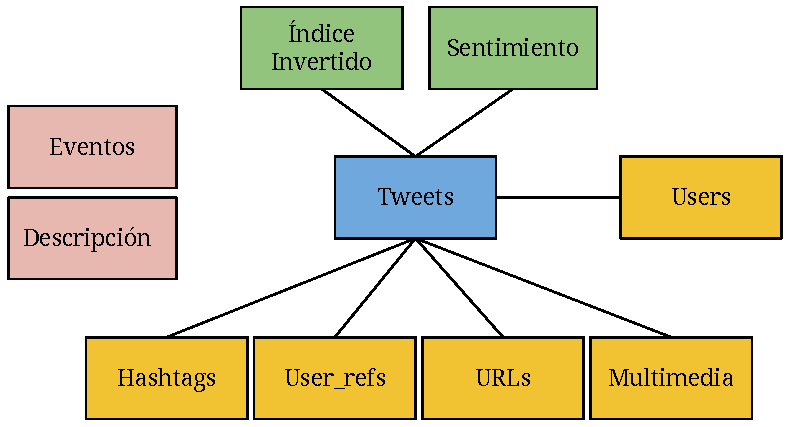
\includegraphics[width=0.8\linewidth]{imagenes/tweetmodel.pdf}
	\caption{Modelo de las tablas generadas diariamente que conforman la base de datos.}
	\label{img:database}
\end{figure}

El \textbf{módulo 2} se encarga del almacenamiento de los \textit{tweets} recolectados y los metadatos asociados. La información se almacena en una base de datos relacional MySQL. 
%
Cada día se crean nuevas tablas para almacenar la información. Esta medida busca evitar tablas de gran tamaño y así optimizar los tiempos de búsqueda en la base de datos. 


La imagen \ref{img:database} muestra las tablas generadas diariamente. 
%
Las tablas de color amarillo almacenan información relacionada al \textit{tweet}. 
%
Los campos de estas tablas guardan información, en su mayoría, proveniente directamente desde Twitter.
%
Algunos de los datos almacenados en estas tablas son generados en el módulo de pre-procesamiento, como la información de geolocalización y una etiqueta que indican si el \textit{tweet} fue publicado por un mismo usuario en un corto periodo de tiempo.

Las tablas de color verde almacenan otra información generada por el sistema.
%
Una de ellas almacena un índice invertido de las palabras que conforman el texto de los \textit{tweet} y la otra almacena el resultado del análisis de sentimiento para cada \textit{tweet}. 
%
Las tablas de color rosado almacenan la información relacionada con las detecciones y son pobladas con la información generada en los módulos 4 y 5 que se describen más adelante. 


Además de las tablas del modelo de la figura~\ref{img:database}, existen otras ``tablas virtuales'' o ``vistas'' destinadas al almacenamiento de datos agregados que son utilizados para la detección de ráfagas y para el almacenamiento de datos precalculados para las visualizaciones.
%
%En el \nameref{anexo:bd} se detalla el esquema de la base de datos y los campos que conforman cada tipo de tabla creada.

\section{Agrupación de \textit{tweets} y generación de señales}

El \textbf{módulo 3} se encarga de preparar los datos para ser procesados en busca de ráfagas.
%
Los \textit{tweets} del \textit{stream} son agrupados en conjuntos etiquetados según el \textit{timestamp} de la fecha de creación. 
%
Cada conjunto de \textit{tweets} representa una ventana de tiempo individual. 
%
Las ventanas de tiempo son alineadas secuencialmente.
%
Cada secuencia de ventanas puede ser representada como una señal discreta, la que es analizada por el módulo siguiente.
%
Como parte de la experimentación se generaron diferentes tipos de señales a partir de algunos atributos de interés específicos. %Por ejemplo, señales conformadas por tweets que mencionaban un mismo país en el mensaje. 
%
Las señales generadas fueron:

\begin{enumerate}
\item Señal de \textit{tweets} con palabras clave: Señal conformada por todos los \textit{tweets} que contienen cualquier palabra relacionada con sismos en cualquier idioma~\footnote{Palabras especificadas en una lista de palabras clave.}. 
\item Señales de localización del usuario: Señales construidas mediante la agrupación de \textit{tweets} publicados por usuarios que indican pertenecer al mismo país en su perfil. Esta agrupación se hace considerando los \textit{tweets} que contienen palabras relacionadas con sismos.
\item Señales de localización considerando el texto: Señales construidas mediante la agrupación de \textit{tweets} que mencionan el mismo país en el texto del mensaje. Esta agrupación se hace considerando los \textit{tweets} que contienen palabras relacionadas con sismos.
\item Señales de idioma: Señales construidas mediante la agrupación de \textit{tweets} escritos en el mismo idioma. Para esto se consideran los \textit{tweets} que contienen palabras relacionadas con sismos.
\item Señales de sentimiento: Dos señales, una que agrupa los \textit{tweets} que reportan sismos y que expresan sentimiento positivo y otra con los \textit{tweets} que reportan sismos y que expresan sentimiento negativo. 
\end{enumerate}

En el capítulo \ref{cap:analisis} se vuelve a mencionar las señales creadas y se presentan los resultados obtenidos a partir de su análisis para detección de sismos.

\section{Procesamiento de señales}

El \textbf{módulo 4} se encarga de procesar las secuencias de ventanas generadas por el módulo anterior y analizarlas en busca de ráfagas.  
%
Para analizar los datos se utiliza una estructura de datos de tabla de hash concurrente en donde se almacenan datos estadísticos asociados a cada ventana de tiempo. Esta estructura permite acceder a los datos en paralelo y mejorar el rendimiento.
%
El detalle de la metodología de detección se explicó previamente en el capítulo \ref{cap:deteccion}.

\section{Descripción de los eventos detectados}

El \textbf{módulo 5} se encarga de la descripción de eventos, es decir, se encarga de procesar la ventana de tiempo donde se detectó una ráfaga para determinar las palabras y los \textit{tweets} que propiciaron ese comportamiento.
%
Con esta información se complementa la información temporal y geográfica asociada a esa ventana de tiempo.
%
En conjunto toda esta información describe un evento, ya que responden a las preguntas sobre el cuándo, dónde y qué es lo que pasó específicamente en cada evento detectado.
%
En el capítulo \ref{cap:casos} se muestra un breve análisis para algunos casos de eventos sísmicos detectados  donde se responden a estas preguntas.  


\section{Aplicación Web}

La aplicación Web se compone por dos partes: el servidor Web (módulo 6) y el frontend que se ejecuta en el browser de los usuarios (módulo 7). 

\subsection{Servidor Web}
El \textbf{módulo 6} corresponde al servidor de la aplicación Web implementado en Python utilizando el \textit{framework} Flask\footnote{\url{http://flask.pocoo.org/}}. El servidor accede directamente a la base de datos y consulta los datos a medida que estos van siendo agregados. Para servir los datos en tiempo real se utiliza un caché con auto-refresco de 1 segundo, que evita sobrecargar el servidor cuando acceden muchas personas al mismo tiempo a la aplicación. 

\subsection{Interfaz Web}
El \textbf{módulo 7} corresponde a la interfaz de la aplicación Web. Para su implementación se utilizaron las siguientes bibliotecas:
\begin{itemize}
\item JQuery.js\footnote{\url{https://jquery.com/}}: Biblioteca javascript para facilitar la manipulación de documentos y las llamadas Ajax. 
\item Bootstrap\footnote{\url{http://getbootstrap.com/}}: Framework para desarrollar aplicaciones responsivas y que funcionan en varios dispositivos.
\item D3.js\footnote{\url{https://d3js.org/}}: Biblioteca javascript para manipular documentos basados en datos y generar visualizaciones interactivas. %
\item Leaflet.js\footnote{\url{http://leafletjs.com/}}: Biblioteca javascript para visualizaciones interactivas usando mapas. 
\item Leaflet.heat\footnote{\url{https://github.com/Leaflet/Leaflet.heat}}: Un plugin que extiende Leaflet para crear mapas de calor. 
\item Leaflet.markercluster\footnote{\url{https://github.com/Leaflet/Leaflet.markercluster}}: Un plugin que extiende Leaflet para agrupar marcadores cercanos entre si y desplegarlos de forma interactiva. 
\end{itemize}

%En la sección \ref{sec:visualizacion} se detallan las visualizaciones utilizadas para presentar los datos y en la sección \ref{sec:aplicacion} se muestran vistas completas de la aplicación y su modo de uso. 
En el capítulo \ref{cap:aplicacion} se detallan las visualizaciones utilizadas para presentar los datos, así como también, vistas completas de la aplicación y su modo de uso. 
\chapter{Aplicación Web}
\label{cap:aplicacion}

Parte del trabajo realizado en esta tesis consiste en el desarrollo de una aplicación Web para presentar la información en tiempo real. 
%
El objetivo principal del desarrollo de esta aplicación no es el diseño del software ni de las interfaces, si no más bien, poner en producción una prueba de concepto que permite validar su utilidad como herramienta de apoyo para los sismólogos del Centro Sismológico Nacional.


La aplicación debía permitir a los usuarios identificar las características de los eventos rápidamente, es decir, identificar la hora y el lugar donde ocurre el sismo y el impacto que tuvo en la red social.
%
Además, para los usuarios e investigadores es muy valioso tener la posibilidad de explorar datos históricos. Para cumplir con este objetivo la aplicación permite pausar el refresco de información y cargar datos recopilados para fechas anteriores.  
%
La aplicación está disponible en \url{http://www.twicalli.cl}.

%A continuación se explican las visualizaciones utilizadas para presentar la información, el diseño que integra cada una de las partes y las interacciones disponibles para que el usuario explore los datos.

\section{Visualización de datos}
\label{sec:visualizacion}

La información que se desea presentar en la aplicación Web consiste principalmente en datos geográficos y temporales. 
%
En la prueba de concepto desarrollada se proponen algunas visualizaciónes básicas para que los usuarios identifiquen rápidamente cuándo está ocurriendo un sismo, dónde se percibe y lo que las personas están comentando al respecto.
%
En esta sección se explica en qué consiste cada una de estas visualizaciones.


	\subsection{Temporales}
	
	\begin{figure}[ht]
	  \centering
	  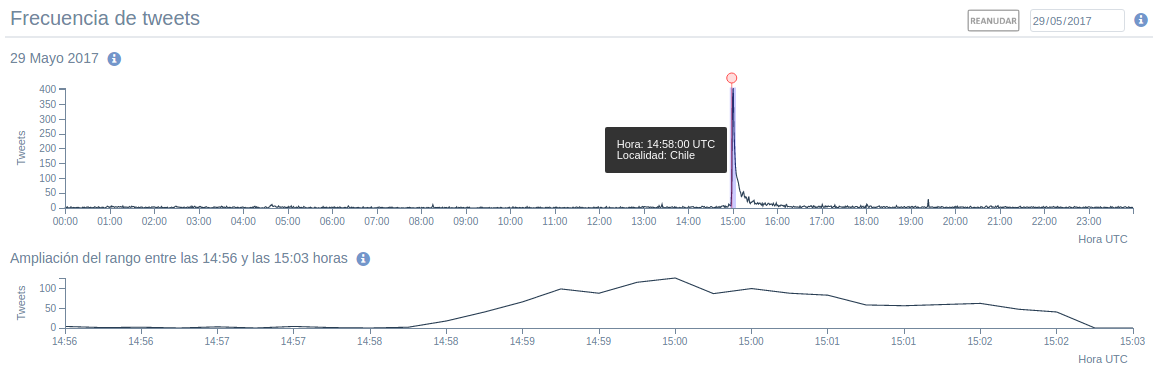
\includegraphics[trim={0 0 0 0}, clip, width=\textwidth]{imagenes/linea_de_tiempo_interactive.png}
	  \caption{Visualización de la frecuencia de \textit{tweets} de un día completo en intervalos de 60 segundos y de la frecuencia de \textit{tweets} de la zona seleccionada en intervalos de 15 segundos.}
	\label{fig:timeline}
	\end{figure}
		
	
	Para visualizar los datos temporales, se utiliza una señal interactiva similar a un gráfico de línea, que se actualiza a medida que pasa el tiempo y que muestra la cantidad de \textit{tweets} publicados en cada momento.
	%
	La imagen \ref{fig:timeline} corresponde a la visualización de los datos recolectados el día 29 de Mayo del 2017.
	%
	La primera señal muestra los datos recolectados en un rango de un día y la segunda señal muestra el rango seleccionado amplificado. Por defecto, están seleccionados los últimos 30 minutos.
		
	Mediante esta visualización es posible identificar rápidamente cambios en el comportamiento típico de los usuarios.
	%
	Además el sistema marca automáticamente los puntos de interés, en este caso, los puntos en donde inicia un sismo. 
	%
	Los usuarios pueden interactuar con esta visualización, ya sea seleccionando un rango de tiempo o haciendo \textit{click} en un punto de interés, lo que permite obtener información más detallada de el periodo de tiempo seleccionado. 
	
	
	\subsection{Geográficos}
	
	\begin{figure}[ht]
	\centering
	\subfloat[Mapa del mundo con \textit{tweets} geolocalizados.]{
		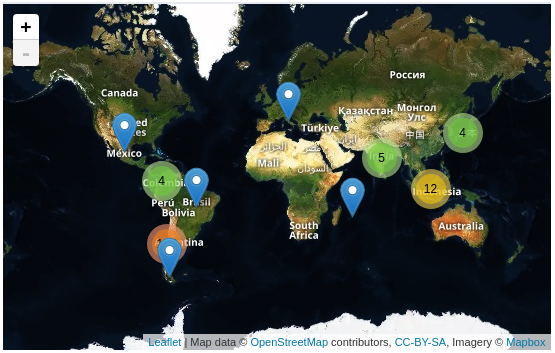
\includegraphics[height=140pt]{imagenes/worldmap.png}
		\label{fig:worldmap-out}
	}
	\hfill
	\subfloat[Mapa ampliado a la zona afectada por el sismo.]{
  		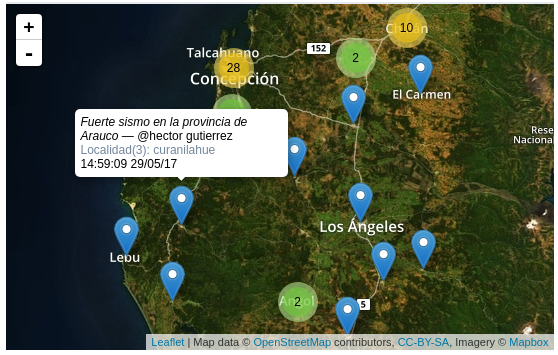
\includegraphics[height=140pt]{imagenes/worldmap-maxzoom.png}
  		\label{fig:worldmap-zoom}
  	}
  	\caption{Mapa interactivo con marcadores para cada tweet geolocalizado y agrupados en base a la distancia que existe entre ellos. Las imagenes corresponden a un sismo ocurrido cerca de  Concepción, Chile, el 29 de Mayo del 2017.}
  	\label{fig:worldmap}
  	\end{figure}
	 	
	  	
	Como se mencionó en el capítulo \ref{cap:geocodificacion} se intenta obtener la mayor cantidad posible de información geográfica. 
	%
	Esto es muy útil ya que, a pesar de no ser 100\% confiable, entrega una buena aproximación de la percepción de un sismo. 
	%
	Saber donde se encuentran los usuarios que reportan un sismo nos permite identificar las áreas afectadas y el alcance geográfico de cada evento. 
	%

	
	Para mostrar esta información se utilizan dos tipos de mapas, el primero consiste en un mapa de calor. 
	%
	La figura \ref{fig:heatmap} visualiza los datos recolectados durante los 15 minutos posteriores a un evento sísmico ocurrido el 29 de Mayo cerca de Concepción. 
	%
	En ella se puede observar la zona en donde se publicaron un mayor número de \textit{tweets} y cómo esto se modifica en el tiempo.
	%
	%Como se puede observar, la imagen muestra una mancha roja un poco más abajo de Santiago. 
	%
	%Esto se debe a que este mapa no se encuentra normalizado. 
	%
	%Sin embargo el usuario tiene la opción de escoger ver el mapa normalizado por población regional, lo que permite observar más claramente que el evento ocurrió más al sur de Chile. 
	%
	%El mapa que muestra los mismos datos pero normalizados por región se muestra en la figura \ref{fig:heatmap-normalizado}.
	
	
	El segundo tipo de mapa consiste en un visualización interactiva del mapa del mundo con marcadores para cada tweet relacionado con alguna localización.
	%
	Para una mejor visualización, los datos se agrupan en base a su cercanía y se van separando en grupos más pequeños a medida que el usuario amplía el mapa o hace \textit{click} en cada grupo. 
	%
	La figura \ref{fig:worldmap-out} muestra la visualización durante un sismo en Chile y la figura \ref{fig:worldmap-zoom} muestra el mismo instante pero con el mapa ampliado a la zona con mayor número de marcadores.
	%
	La visualización permite identificar rápidamente los lugares afectados, en este caso, en el mapa \ref{fig:worldmap-out} se identifica un grupo grande en Chile y a medida que se amplía esa zona, en el mapa \ref{fig:worldmap-zoom} se identifica un grupo numeroso en Concepción (ciudad muy cercana al epicentro) y las ciudades aledañas.
	
	\begin{figure}[!ht]
	  \centering
	  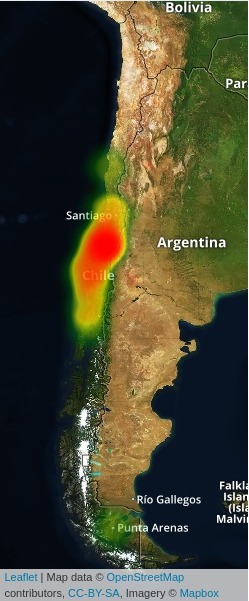
\includegraphics[trim={0 0 0 0}, clip, width=0.4\textwidth]{imagenes/heatmap.png}
	  \caption{Mapa de calor construido a partir de las coordenadas geográficas inferidas de los \textit{tweets} publicados durante un sismo en Concepción}
	\label{fig:heatmap}
	\end{figure}
  	

\section{Usuarios de la Aplicación}

Los usuarios finales de la aplicación son:

\begin{enumerate}
\item Sismólogos de las oficinas del Centro Sismológico Nacional de la Universidad de Chile (CSN)
\item Personas no expertas en sismología que deseen visitar el sitio Web
\end{enumerate}

\section{Diseño de la Aplicación}

El objetivo principal de la aplicación Web es presentar los datos a los usuarios expertos, es decir, a los sismólogos de las oficinas del CSN. 
%
La aplicación será visualizada en las pantallas de monitorización ocupando pantallas ordenadas verticalmente, además se desea poder extraer la información relevante sin la necesidad de interacción.
%
Por otro lado, la aplicación que queda disponible para el resto de los usuarios debe ser fácil de comprender. 


Es de interés poder observar los datos en tiempo real y también se desea poder explorar la información de eventos pasados. 
%
Para cada evento se presenta información de geolocalización. 


Teniendo en cuenta los puntos antes mencionados se desarrollan dos vistas de la aplicación que presentan la misma información. 
% 
Las figuras \ref{fig:webapp} y \ref{fig:webapp_csn} muestran la vista de la aplicación disponible de manera pública y la utilizada por el CSN respectivamente. 
%
En ella se observan las visualizaciones descritas en la sección \ref{sec:visualizacion} y el listado de \textit{tweets}, que permite a los usuarios comprender mejor el evento. 

	\begin{figure}[ht]
	  \centering
	  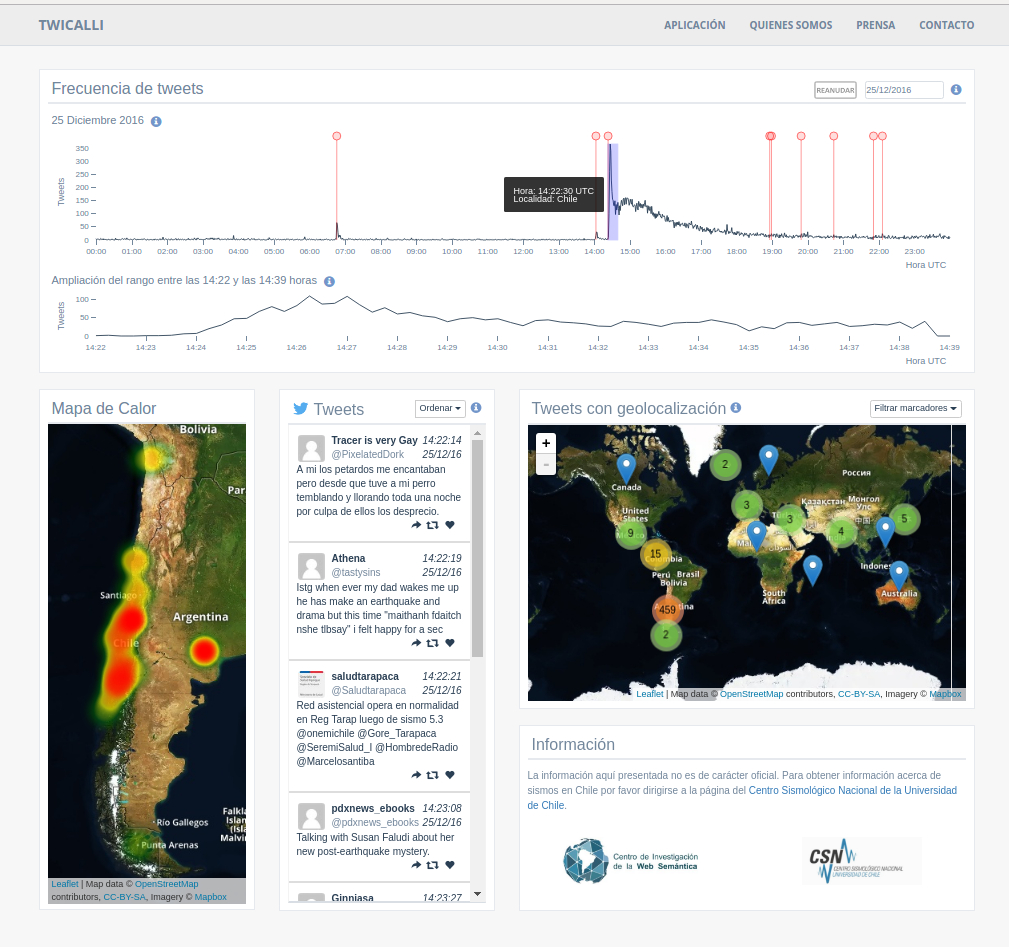
\includegraphics[trim={0 0 0 0}, clip, width=\textwidth]{imagenes/aplicacionexplorar.png}
	  \caption{Vista de la aplicación Web disponible públicamente}
	\label{fig:webapp}
	\end{figure}
	
	\begin{figure}[ht]
	  \centering
	  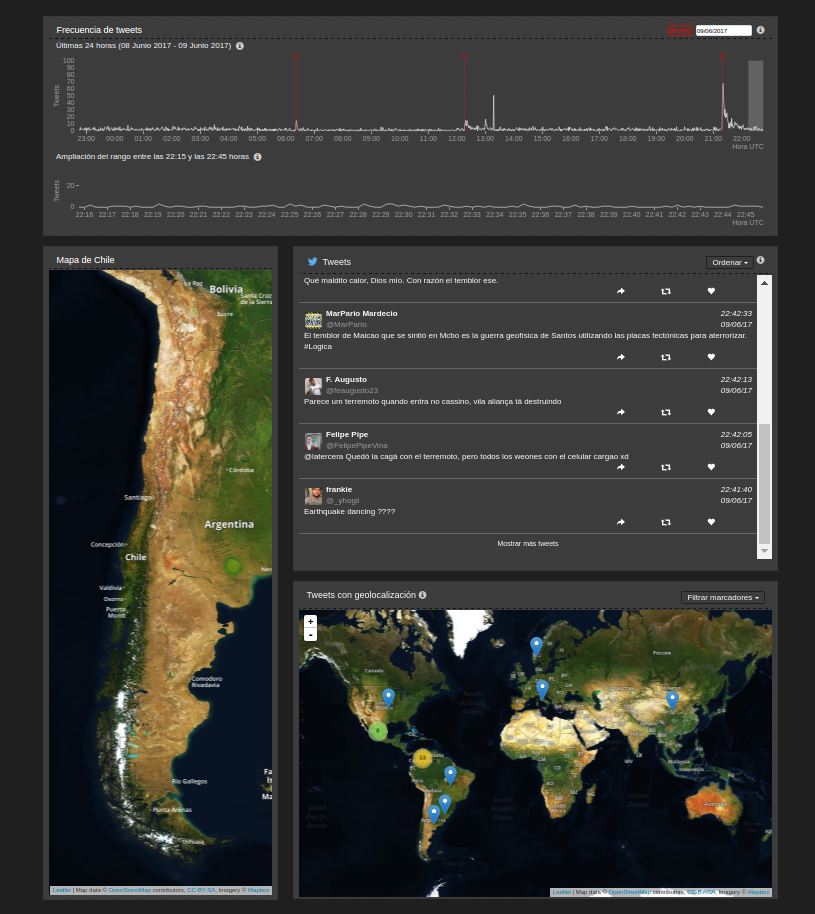
\includegraphics[trim={0 0 0 0}, clip, width=\textwidth]{imagenes/aplicacionexplorar_csn.png}
	  \caption{Vista de la aplicación Web utilizada por usuarios del CSN}
	\label{fig:webapp_csn}
	\end{figure}


Gracias a las iteraciones y la retroalimentación de los usuarios expertos se pudo identificar algunas mejoras, principalmente en la vista que visualizarán en las pantallas del CSN:

\begin{enumerate}
\item Preferencia por el uso de un mapa en el que se distinga el relieve del terreno y las fallas geográficas del borde costero chileno.
\item Selección de los colores utilizados en el mapa de calor y los marcadores para que no se confundan con los colores del mapa. 
\item Preferencia por el uso de una paleta de colores oscura para el fondo de la aplicación, debido a que el fondo blanco en las pantallas de monitorización cansa la vista.
\end{enumerate}


\section{Interacciones}

La aplicación Web por defecto presenta los datos en tiempo real correspondiente a los últimos 30 minutos.
La línea de tiempo del día completo se actualiza cada 1 minuto y la línea de tiempo amplificada se actualiza cada 15 segundos. 
Además cada 1 segundo se consulta si hay nuevos \textit{tweets} y de ser así se dibujan en los mapas y en la parte superior de lista de tweets.  

Los usuarios pueden interactuar con la aplicación y en caso de hacerlo la actualización automática se detiene, pudiendo reanudarse en cualquier momento haciendo \textit{click} en el botón \textit{reanudar} de la parte superior derecha de la línea de tiempo. 

Las interacciones disponibles son: 

\begin{itemize}
\item Seleccionar un largo de tiempo de la línea de tiempo principal. Esto permite actualizar la información en el resto de la página, mostrando el rango de tiempo amplificado y la información de los \textit{tweets} publicados durante ese rango de tiempo. 
\item Hacer \textit{click} en un marcador rojo de la línea de tiempo principal, el cual representa la ocurrencia de un evento. Esta acción selecciona automáticamente el rango en el que aumentó el número de \textit{tweets} relacionados a ese evento y actualiza la información del resto de las visualizaciones de la misma forma que la interacción anterior. 
\item Hacer \textit{click} en los marcadores del mapa que están agrupados para desagruparlos.
\item Hacer \textit{click} en los marcadores desagrupados para mostrar información específica del \textit{tweet}.
\item Seleccionar una fecha para mostrar información de un día anterior. 
\end{itemize}




%Análisis Experimental
%	Conjuntos de datos oficiales 
%	Criterios de la evaluación
%	Resultados 


\chapter{Análisis Experimental}
\label{cap:analisis}

\jm{Introducción del capítulo, objetivos del capítulo}
En este capítulo se analiza la efectividad de la metodología de detección de sismos propuesta. 
%
El análisis realizado comienza identificando la configuración inicial óptima del algoritmo. 
%
definir los datos con los cuales se realiza la validación (\textit{ground truth}) 

se comparan los resultados obtenidos al utilizar diferentes conjuntos de atributos de interés\footnote{Revisar el capítulo \ref{cap:deteccion} para más detalles de la metodología de detección y los conceptos asociados}.


se comparan los resultados obtenidos considerando una variedad de atributos como elementos de interés.


\section{Preparación del experimento}

\jm{Introducción de la sección}

	\subsection{Conjunto de datos de \textit{Twitter}}
	
		El flujo de datos $\mathcal{F}$ está conformado por \textit{tweets} publicados en \textit{Twitter} desde el 25 de Enero al 25 de Octubre del 2016 (9 meses). Técnicamente, sólo es posible acceder a una muestra del flujo público completo, por lo tanto, los datos son recuperados ya filtrados en base a palabras clave o atributos de interés especificados en $\mathcal{K}$ (en vez de obtener todo el flujo de datos y luego filtrar).  Para obtener los datos se utiliza la API para acceder al \textit{stream} público, tal como se explica en la sección \ref{sec:recoleccion} sobre recolección de datos. Los \textit{tweets} son procesados de manera estándar, normalizando el texto y removiendo duplicados (igual ID). El procesamiento es realizado considerando múltiples idiomas, incluyendo idiomas orientales, como chino, japonés, y persa. En total, el conjunto de datos utilizado para el análisis está compuesto por 53.557.475 \textit{tweets}.
		
		Los \textit{tweets} con coordenadas geográficas asociadas representan sólo el 8\% del conjunto de datos. La información geográfica fue incrementada mediante la incorporación de información de ubicación inferida, de forma similar a como lo hacen Robinson et al.~\cite{robinson2013sensitive}. Específicamente, se utiliza un índice geográfico para extraer nombres de localidades a partir del texto de los mensajes y de los perfiles de usuario. La extracción de datos se detalla en la sección \ref{sec:geocodificacion}. Utilizando este procedimiento, es posible geolocalizar el 53,6\% de la colección (28.723.948 \textit{tweets}).
		
	\subsection{Conjuntos de datos utilizados como \textit{Ground Truth}}
	
		Para verificar los resultados se utilizaron catálogos de sismos disponibles públicamente, uno correspondiente a una red de sensores global y otro a una red de sensores local. Se utilizaron las detecciones correspondientes al mismo periodo de 9 meses del conjunto de datos recolectados desde \textit{Twitter}. Ambos catálogos se constituyen por reportes oficiales y describen la localidad estimada del epicentro del sismo y la magnitud ~\cite{usgs:magnitude}.
		
\begin{description}
\item[Global (USGS):] 
		Catálogo construido por el \textit{Geological Survey} de Estados Unidos~\cite{usgs:data}. Este catálogo es muy completo para sismos de magnitud superior a $4.5$ ocurridos en diferentes partes del mundo ~\cite{earle2010omg}. Sin embargo, en el caso de sismos con magnitud inferior a $4.5$, los reportes consisten principalmente en eventos ocurridos en regiones específicas de Estados Unidos que tienen mejor cobertura de sensores. Para el periodo de estudio la USGS reportó 9.470 sismos con magnitud $\geq$ $4.0$ en todo el mundo. Se utilizó este conjunto de datos para evaluar el algoritmo propuesto y comparar su desempeño con otros sistemas que tienen cobertura mundial.

\item[Catálogo Local (GUC):]
		Este catálogo está focalizado en Chile y es generado por la Agencia Sismológica Nacional de Chile~\cite{guc:data}. Los reportes se basan en las detecciones realizadas por la extensa y densa red de sensores del GUC que es muy completa para sismos en Chile. Además de la información del epicentro y magnitud, este catálogo reporta la intensidad, indicando cuándo un sismo fue percibido por las personas y cuánto daño produjo (en la escala de intensidad modificada de Mercalli~\cite{usgs:mercalli}).
		Para el periodo de tiempo del estudio el GUC reportó 662 sismos de magnitud $\geq$ $4.0$, 476 de ellos clasificados como \textit{sismos sensibles}. Se utilizó este conjunto de datos para evaluar el algoritmo propuesto y comparar su desempeño con otros sistemas que tienen cobertura local. 
		
\end{description}
		
		Cabe destacar que durante el periodo de estudio, el GUC reportó 1.373 sismos en Chile ($\geq$ $3.6$) y el USGS reportó sólo 436 sismos en Chile con la misma magnitud (sólo 32\% de cobertura). Esto corrobora la necesidad de tener fuentes de información complementaria para completar la cobertura de sismos en áreas que no están bien cubiertas por las redes de sismología globales o locales. 
		
	\subsection{Ajuste de parámetros iniciales óptimos}

	La metodología de detección de sismos propuesta requiere que se fijen 3 parámetros iniciales:
	\begin{enumerate}
		\item El umbral para detectar sismos $\theta$.
		\item La lista de atributos que definen un elemento de interés ($K$).
		\item El tamaño de la ventana de tiempo ($T$).
	\end{enumerate}
	
	A continuación se detalla cómo se determinaron los valores utilizados para realizar la configuración inicial de cada uno de estos parámetros. 

	\subsubsection*{1. Umbral para detectar sismos ($\theta$)}
	%
	Para determinar las variaciones significativas en el flujo $\mathcal{F}$ se identificó el valor óptimo para el umbral $\theta$ empíricamente. 
	%
	Utilizando una muestra de datos de 2 meses, se probó el sistema de detección usando diferentes valores de $\theta$ y se seleccionó el valor que maximiza el {\em F-measure}.
	%
	La tabla~\ref{table:zscore} muestra los resultados obtenidos y el valor seleccionado $\theta=1.5$.
	\begin{table}
\centering
\begin{tabular}{cccc}
\toprule
{z-score ($\theta$)} & {Precision} & {Recall} & {F-Measure} \\ 
\midrule
{0.5}    & {48.1\%}     & {79.9\%}  & {60.1\%}  \\ 
{1.0}    & {62.6\%}     & {65.0\%}  & {63.8\%}  \\ 
{\bf 1.5}    & {\bf 88.3\%}     & {\bf 54.2\%}  & {\bf 67.1\%}  \\
{2.0}    & {92.3\%}     & {29.0\%}  & {44.2\%}  \\ 
\bottomrule
\end{tabular}
\caption{Comportamiento del algoritmo utilizando diferentes valores para el umbral de detecci\'on de sismos $\theta$.}
\label{table:zscore}
\end{table}



	\subsubsection*{2. Listado de atributos que definen un elemento de interés ($K$)} 
	Como se mencionó previamente, en esta adaptación los elementos de interés ($K$) son una lista de palabras clave relacionadas con la ocurrencia de sismos.
	%
	En esta tesis se extendió la lista de palabras entregada por investigadores del USGS, que fue usada por Earle et al.~\cite{earle2012twitter} y Avvenuti et al.~	\cite{avvenuti2014earthquake,avvenuti2014ears}.
	%
	Sin embargo, a diferencia de los sistemas anteriores, la lista de palabras utilizada se construyó intentando incluir la mayor cantidad posible de palabras relacionadas con ocurrencias de sismos en cualquier idioma, incluso si incluía términos ambiguos (es decir, términos que a veces son utilizados en otros contextos).
	%
	Los mensajes ruidosos que puedan ser obtenidos al usar términos ambiguos no afectan el rendimiento de este método ya que es tolerante al ruido. 
	%
	Por ejemplo, la palabra ``quake'' puede ser usada para referirse a un videojuego o al personaje de un comic con el mismo nombre, o la palabra ``terremoto'' que en Chile también es utilizada para referirse a una bebida alcohólica típica y muy consumida durante las celebraciones nacionales. 
	%	
	La lista de palabras está compuesta por los términos listados en la figura \ref{img:keywords}. 
	%
	En caso de ser necesario modificar los términos de la lista, ésta puede ser actualizada dinámicamente.
	
	\begin{figure}[h!]
	\centering
	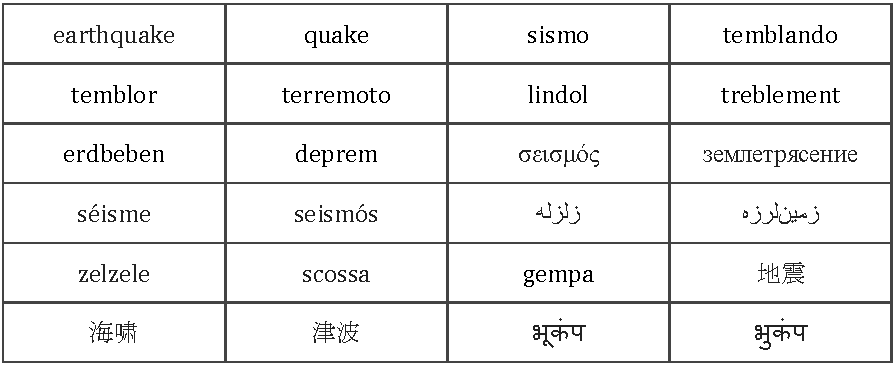
\includegraphics[width=0.8\textwidth]{imagenes/Keywords.pdf}
	\caption{Palabras clave utilizadas para recolectar \textit{tweets} relacionados con sismos.}
	\label{img:keywords}
	\end{figure}
	
	
	Además de las palabras clave relacionadas con sismos, se realizaron experimentos en los cuales además de las palabras clave, también se consideraban otros atributos para determinar si un elemento era de interés o no. 
	%
	De esta forma se pudo analizar la señal discreta asociada a diferentes tipos de atributos y determinar si estos agregaban valor a la detección o no. 
	%
	Entre estos atributos se encuentran:
	\begin{itemize}
	\item Sentimiento positivo del \textit{tweet}.
	\item Sentimiento negativo del \textit{tweet}.
	\item Idioma en el cual fue escrito el \textit{tweet}
	\item País mencionado en el texto del \textit{tweet}.
	\item País mencionado en la localidad de perfil del usuario que escribió el \textit{tweet}.
	\end{itemize}

	\begin{figure}[ht]
  	\centering
  	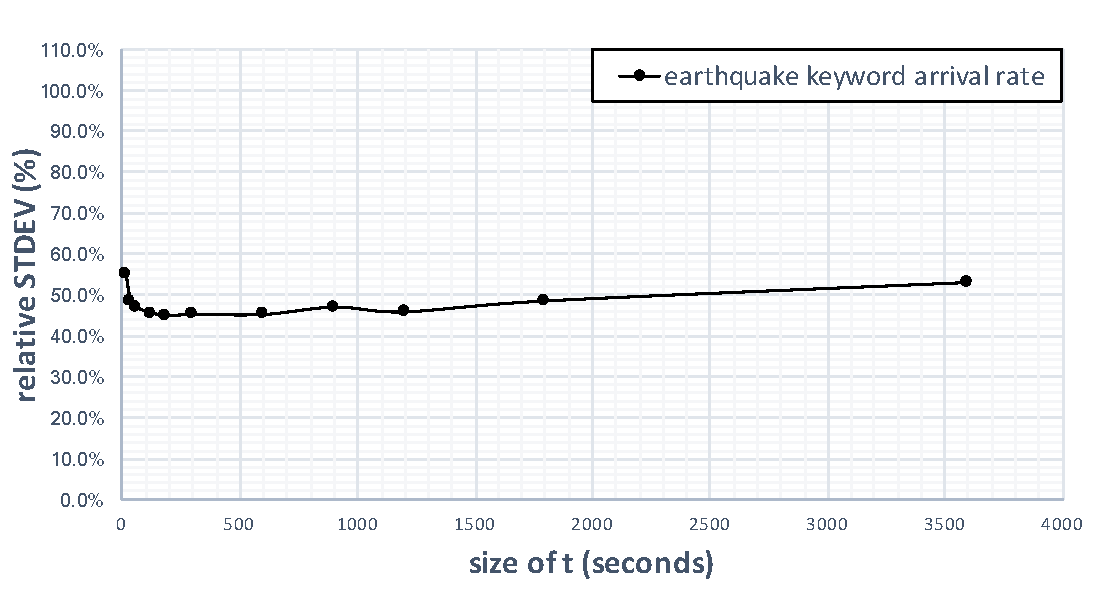
\includegraphics[trim={5 0 5 10}, clip, width=\textwidth]{imagenes/02_Poise_Analysis_WindowSize_solo.pdf}
  	\caption{Desviación estándar relativa de la señal que considera las palabras clave relacionadas con sismos para diferentes tamaños de ventana de tiempo (en segundos)}
	\label{fig:window_size}
	\end{figure}

	\subsubsection*{(3) Tamaño de la ventana de tiempo ($T$)} 
	El tamaño de la ventana corresponde al largo del tiempo (en segundos) de cada conjunto de \textit{tweets} en los cuales son divididos los datos de la entrada para ser procesados por el algoritmo.
	%
	Este parámetro se determina analizando el flujo de la entrada y seleccionando un valor para $T$ que minimiza la desviación estándar relativa, es decir, cuando la frecuencia de aparición es más estable. 
	%
	Intuitivamente, si la ventana de tiempo es muy pequeña, los mensajes que contengan elementos en $K$ estarán distribuidos de forma más aleatoria en cada ventana. 	
	%
	Esto significa que habrían ventanas de tiempo sin ninguna ocurrencia y otras con varias ocurrencias.
	%
	Mientras más grande sea la ventana de tiempo, más factible es poder estimar la frecuencia en la ventana siguiente. 
	%
	Para determinar el valor de $T$ se utilizó el siguiente procedimiento, descrito en~\cite{guzman2013line}:

	\begin{itemize}
	\item Para el flujo de entrada dado, se calcula la velocidad de llegada relativa de ventanas sucesivas $w_i$ de tamaño $T$.

	\item Se repite este proceso para diferentes tamaños de ventana $T$ en el rango de $0$ hasta $3\,600$ segundos (una hora) para un periodo de 2 meses y se selecciona el $T$ con la desviación estándar relativa más pequeña. En este caso el valor de tamaño de ventana que minimiza la desviación estándar corresponde a los valores para $T \geq 300$ segundos, tal como se muestra en la figura~\ref{fig:window_size}.

	\end{itemize}

	Además, para disminuir los tiempos de detección, el sistema ejecuta dos procesos paralelos idénticos desfasados en $150$ segundos uno del otro y con ello asegurar un tiempo de detección de máximo 5 minutos. 

		
\section{Evaluación}

En esta sección se presenta la evaluación del método de detección de sismos propuesto. La evaluación se realizó utilizando 5 tipos de variaciones del flujo de entrada $\mathcal{F}$ creado a partir de mensajes que contienen palabras relacionadas con sismos $\mathcal{K}$. Estos 5 tipos de flujos son:

\begin{description}

\item[Palabras clave de sismos:] Este flujo de mensajes genera una señal que representa la velocidad de llegada relativa de mensajes que contienen algún elemento en $\mathcal{K}$, donde $\mathcal{K}$ corresponde a la lista de palabras relacionadas con sismos. 
\item[Geolocalización a partir del texto:] Los \textit{tweets} seleccionados usando las palabras clave relacionadas con sismos se etiquetan con los países mencionados en el corpus del \textit{tweet}. Estos \textit{tweets} son separados en distintos flujos de mensajes en base a las etiquetas, es decir, un flujo por cada país. Luego se analizan los flujos asociados a cada país en forma de señales generadas a partir de la velocidad de llegada relativa de los mensajes. 
\item[Geolocalización a partir del perfil del usuario:] Creado de manera similar a las señales de \textit{geolocalización a partir del texto}, con la diferencia que las etiquetas de localidades son extraídas desde el perfil del usuario.
\item[Idioma:] Creado de manera similar a las señales de \textit{geolocalización a partir del texto y del perfil del usuario}, con la diferencia que las etiquetas corresponden a los idiomas utilizados en el corpus del \textit{tweet}. Los diferentes flujos son analizados de la misma forma, generando señales representando la velocidad de llegada relativa de los mensajes. 
\item[Sentimiento:] Los \textit{tweets} seleccionados usando las palabras clave relacionadas con sismos son analizados para detectar si corresponden a un mensaje con sentimiento positivo o negativo. El análisis de sentimiento se describe con más detalle en la sección \ref{sec:sentimiento}. Los \textit{tweets} etiquetados se separan en dos flujos, un flujo con los mensajes con polaridad positiva y otro con los mensajes con polaridad negativa. Luego se analizan las señales generadas calculando la velocidad de llegada relativa de los \textit{tweets} que componen cada flujo.

\end{description}

\subsection{Metodología de evaluación}

La evaluación se realizó intentando satisfacer los criterios utilizados en los trabajos previos con los cuales se desea comparar el sistema~\cite{sakaki2010earthquake,avvenuti2014ears,robinson2013sensitive,earle2012twitter}. Se replicaron los experimentos usando el conjuntos de datos de \textit{Twitter} descrito previamente y los datos utilizados como \textit{ground truth}, los cuales son equivalentes a los utilizados en las evaluaciones de los trabajos previos. Sin embargo no fue factible replicar los otros sistemas para compararlos utilizando exactamente los mismos datos. Esto se debe principalmente a que no tenemos acceso al código fuente, modelos ni detalles de implementación de esos sistemas. Así como también debido a los altos costos asociados a los enfoques supervisados (es decir, etiquetado de datos y parametrización), que se describen en el capítulo \ref{cap:marco}. Por lo tanto, se reportan los resultados y luego se comparan de la forma más cercana posible a los resultados reportados por sistemas similares.

Sin embargo, hay algunas consideraciones relacionadas al uso de los catálogos de sismos utilizados como \textit{ground truth} en los sistemas basados en datos sociales:

\begin{enumerate}
\item  \textit{No todos los sismos en un catálogo fueron percibidos por las personas}. Por lo tanto, cualquier sistema que dependa de los \textit{sensores sociales o ciudadanos} puede potencialmente detectar sólo  un subconjunto de sismos que fueron efectivamente percibidos por humanos. Idealmente, un \textit{ground thruth} perfecto para sistemas basados en datos sociales debería considerar únicamente los sismos que fueron percibidos por personas. 
\item \textit{No todos los sismos en un catalogo que fueron sentidos por personas están etiquetados oficialmente como ``sismos sensibles''}. Esta discrepancia ocurre cuando las personas encargadas de reportar oficialmente la intensidad del sismo no advierten el suceso (principalmente durante sismos de baja intensidad). Idealmente, un \textit{ground truth} perfecto debería tener todos los sismos percibidos etiquetados como \textit{sismos sensibles}. 
\item \textit{Los catálogos de sismos con magnitud inferior a 4.0 de las agencias sismológicas no están siempre completas (no tienen \textit{recall} perfecto}. Los reportes de sismos están basados en detecciones realizadas por múltiples sensores sismográficos que componen una red. Sin embargo, si un sismo ocurre en un área sin sismógrafos o con una baja densidad de sensores, estos no son reportados. Esto se refiere a la integridad el catálogo y también se discute en \cite{earle2010omg}. 
\end{enumerate}

\begin{table*}[!h]
\centering
\begin{tabular}{lcccc}
    \toprule
    \textbf{Trabajo}  & \textbf{Técnica} & \textbf{Cobertura} & \textbf{Palabras} & \textbf{Activo} \\ 
    \midrule
    Twicalli & No Supervisado & Mundial & \begin{tabular}[c]{@{}c@{}} earthquake, sismo, quake, \\temblor,
    temblando, gempa, \\lindol, tremblement, erdbeben, \\ deprem, seismós, séisme, \\ 
    zelzele, terremoto, scossa  \\ y traducciones de sismo en \\ Japonés, Chino, Griego \\ y Persa
    \end{tabular} & Si \\ 
    \midrule
    EARS & Supervisado & Italia  & scossa, terremoto & Si \\ 
    \midrule
    Sakaki et. al. & Supervisado & Japón  & earthquake, shaking & Si \\ 
    \midrule
    Earle et al. & No Supervisado & Mundial & \begin{tabular}[c]{@{}c@{}} earthquake, gempa, sismo, \\temblor, terremoto \end{tabular} & No \\
    \midrule
    ESA & Supervisado & \begin{tabular}[c]{@{}c@{}}Australia \& \\ Nueva Zelanda\end{tabular} & earthquak,
    \#eznq & Si \\ 
    \bottomrule
\end{tabular}
\caption{Resumen del alcance de los estudios similares en el Estado del Arte.}
\label{table:comparison} 
\end{table*}


Para lidiar con estas limitaciones y en un intento de proveer resultados comparables con los trabajos previos (resumidos en la tabla \ref{table:comparison}), se proponen tres criterios de evaluación diferentes:

\begin{description}

\item[Estricto] Esta evaluación considera como \textit{ground truth} los sismos listados en los catálogos global y local. Independientemente a si está o no etiquetado como ``sismo sensible'' (un criterio similar fue utilizado por Earl et al.~\cite{earle2010omg}, Avvenuti et al.~\cite{avvenuti2014earthquake,avvenuti2014ears}).

\item[Super-estricto] Esta evaluación considera como \textit{ground truth} únicamente a los sismos listados en los catálogos global y local que han sido reportados como ``sismos sensibles'' (un criterio similar es utilizado por Sakaki et al.~\cite{sakaki2013tweet} y Avvenuti et al.~\cite{avvenuti2014earthquake,avvenuti2014ears}).

\item[Moderado] Esta evaluación considera como \textit{ground truth} a los ``sismos sensibles'' (al igual que el criterio super-estricto) y además cualquier sismo detectado por el sistema basado el redes sociales si, y solo si, este coincide con un sismo ``no sensible'' listado en los catálogos de sismos. En este criterio, que es más flexible, se asume que si los usuarios de Twitter comentan acerca de un sismo, y al mismo tiempo los sismógrafos detectan un sismo, entonces el sismo puede ser considerado como un sismo que efectivamente ocurrió.

\end{description} 

\section{Resultados}
\label{sec:results}

\begin{table}[!ht]
\centering
  \begin{tabular}{c|lcccccc}
    \toprule
    & \multicolumn{1}{l}{{Tipo de señal (USGS)}}&\multicolumn{1}{c}{{TP}}&\multicolumn{1}{c}{{FP}}&\multicolumn{1}{c}{{FN}}&\multicolumn{1}{c}{{Precisión}}&\multicolumn{1}{c}{{\em Recall}}&\multicolumn{1}{c}{{\em F-Measure}}\\
    \midrule
    \parbox[t]{1.5mm}{\vspace{-0.3cm}\multirow{7}{*}{\rotatebox[origin=c]{90}{{$\geq$ 4,0}}}}
    & {Palabras clave de sismos} & 7528 & 398 & 2469 & {0,95} &  {0,75} & {0,84} \\
	& {País en el texto } & 7878 & 503 & 2119 & {0,94} & {0,79} & {0,86} \\    
    & {País del usuario} & 8096 & 404 & 1901  & {{\bf 0,95}} & {{\bf 0,81}} & {\bf 0,88} \\
    & {País del tweet} & 1342 & 690 & 8655 & {0,66} & {0,13} & {0,22} \\  
    & {Sentimiento Positivo} & 244 & 163 & 9753 & {0,60} &	{0,02} & {0,05} \\
    & {Sentimiento Negativo} & 786 & 356 & 9211 & {0,69} &	{0,08} & {0,14} \\
    & {Idioma} & 7181 & 772 & 2816 & {0,90} & {0,72} & {0,80} \\
    \midrule
    \parbox[t]{1.5mm}{\vspace{-0.3cm}\multirow{7}{*}{\rotatebox[origin=c]{90}{{$<$4,0}}}}
	& {Palabras clave de sismos} & 1010 & 738 & 4751 & {0,58} & {0,18} & {0,27} \\
	& {País en el texto} & 4343 & 3928 & 1418 & {0,53} & {0,75} & {0,62} \\
	& {País del usuario} & 4573 & 3853 & 1188 & {\bf 0,54} & {\bf 0,79} & {\bf 0,65} \\
	& {País del tweet} & 775 & 727 & 4986 & {0,52} & {0,14} & {0,21} \\ 
	& {Sentimiento Positivo} & 130 & 173 & 5631 & {0,43} & {0,02} & {0,04} \\
	& {Sentimiento Negativo} & 449 & 445 & 5312 & {0,50} &	{0,08} & {0,14} \\
	& {Idioma} & 4013 & 3480 & 1748 & {0,54} & {0,70} & {0,61} \\
    \bottomrule
  \end{tabular}
  \caption{{Evaluación estricta considerando el catálogo del USGS compuesto por 15758 registros de sismos}}
  \label{table:global-strict}
\end{table}
%
%


\begin{table}[!ht]
\centering
  \begin{tabular}{c|lcccccc}
    \toprule
    & \multicolumn{1}{l}{{Tipo de señal (GUC)}}&\multicolumn{1}{c}{{TP}}&\multicolumn{1}{c}{{FP}}&\multicolumn{1}{c}{{FN}}&\multicolumn{1}{c}{{Precisión}}&\multicolumn{1}{c}{{\em Recall}}&\multicolumn{1}{c}{{\em F-Measure}}\\
    \midrule
    \parbox[t]{1.5mm}{\vspace{-0.3cm}\multirow{7}{*}{\rotatebox[origin=c]{90}{{$\geq$ 4,0}}}}
    & {Palabras clave de sismos} & 389 & 1 & 273 & {{\bf 1,00}} &  {{\bf 0,59}} & {{\bf 0,74}} \\
	& {País en el texto } & 269 & 11 & 393 & {0,96} & {0,41} & {0,57} \\    
    & {País del usuario} & 121 & 8 & 541  & {0,94} & {0,18} & {0,31} \\
    & {País del tweet} & 77 & 64 & 585 & {0,55} & {0,12} & {0,19} \\  
    & {Sentimiento Positivo} & 2 & 1 & 660 & {0,68} &	{0,00} & {0,01} \\
    & {Sentimiento Negativo} & 23 & 2 & 639 & {0,92} &	{0,04} & {0,07} \\
    & {Idioma} & 171 & 4 & 491 & {0,98} & {0,26} & {0,41} \\
    \midrule
    \parbox[t]{1.5mm}{\vspace{-0.3cm}\multirow{7}{*}{\rotatebox[origin=c]{90}{{$<$4,0}}}}
	& {Palabras clave de sismos} & 75 & 4 & 3759 & {0,95} & {0,02} & {0,04} \\
	& {País en el texto} & 449 & 88 & 3385 & {\bf 0,84} & {\bf 0,12} & {\bf 0,21} \\
	& {País del usuario} & 160 & 29 & 3674 & {0,85} & {0,04} & {0,08} \\
	& {País del tweet} & 112 & 131 & 3723 & {0,46} & {0,03} & {0,06} \\ 
	& {Sentimiento Positivo} & 1 & 2 & 3833 & {0,33} & {0,00} & {0,00} \\
	& {Sentimiento Negativo} & 14 & 8 & 3820 & {0,64} &	{0,00} & {0,01} \\
	& {Idioma} & 239 & 40 & 3597 & {0,86} & {0,06} & {0,12} \\
    \bottomrule
  \end{tabular}
  \caption{{Evaluación estricta considerando el catálogo del CSN compuesto por 4496 registros de sismos}}
  \label{table:local-strict}
\end{table}


\begin{table}[!ht]
\centering
  \begin{tabular}{c|lcccccc}
    \toprule
    & \multicolumn{1}{l}{{Tipo de señal (GUC)}}&\multicolumn{1}{c}{{TP}}&\multicolumn{1}{c}{{FP}}&\multicolumn{1}{c}{{FN}}&\multicolumn{1}{c}{{Precisión}}&\multicolumn{1}{c}{{\em Recall}}&\multicolumn{1}{c}{{\em F-Measure}}\\
    \midrule
    \parbox[t]{1.5mm}{\vspace{-0.3cm}\multirow{7}{*}{\rotatebox[origin=c]{90}{{$\geq$ 4,0}}}}
    & {Palabras clave de sismos} & 170 & 1 & 31 & {{\bf 0,99}} &  {{\bf 0,85}} & {{\bf 0,91}} \\
	& {País en el texto } & 129 & 3 & 72 & {0,98} & {0,64} & {0,78} \\    
    & {País del usuario} & 65 & 2 & 136  & {0,97} & {0,32} & {0,49} \\
    & {País del tweet} & 35 & 38 & 166 & {0,48} & {0,17} & {0,26} \\  
    & {Sentimiento Positivo} & 2 & 0 & 199 & {1,00} & {0,01} & {0,02} \\
    & {Sentimiento Negativo} & 13 & 0 & 188 & {1,00} &	{0,07} & {0,12} \\
    & {Idioma} & 74 & 3 & 127 & {0,96} & {0,37} & {0,53} \\
    \midrule
    \parbox[t]{1.5mm}{\vspace{-0.3cm}\multirow{7}{*}{\rotatebox[origin=c]{90}{{$<$4,0}}}}
	& {Palabras clave de sismos} & 10 & 0 & 56 & {1,00} & {0,15} & {0,26} \\
	& {País en el texto} & 15 & 1 & 51 & {\bf 0,94} & {\bf 0,23} & {\bf 0,37} \\
	& {País del usuario} & 4 & 4 & 62 & {0,50} & {0,06} & {0,11} \\
	& {País del tweet} & 4 & 3 & 62 & {0,57} & {0,06} & {0,11} \\ 
	& {Sentimiento Positivo} & 0 & 0 & 66  & {0,00} & {0,00} & {0,00}  \\
	& {Sentimiento Negativo} & 0 & 0 & 66  & {0,00} & {0,00} & {0,00}  \\
	& {Idioma} & 3 & 1 & 63 & {0,75} & {0,05} & {0,09} \\
    \bottomrule
  \end{tabular}
  \caption{{Evaluación super-estricta usando el catálogo chileno del GUC de ``sismos sensibles'' conformado por 267 registros de sismos.}}
  \label{table:super-strict}
\end{table}


\begin{table}
\centering
  \begin{tabular}{c|lcccccc}
    \toprule
    & \multicolumn{1}{l}{{Tipo de señal (GUC)}}&\multicolumn{1}{c}{{TP}}&\multicolumn{1}{c}{{FP}}&\multicolumn{1}{c}{{FN}}&\multicolumn{1}{c}{{Precisión}}&\multicolumn{1}{c}{{\em Recall}}&\multicolumn{1}{c}{{\em F-Measure}}\\
    \midrule
    \parbox[t]{1.5mm}{\vspace{-0.3cm}\multirow{7}{*}{\rotatebox[origin=c]{90}{{$\geq$ 4,0}}}}
    & {Palabras clave de sismos} & 388 & 1 & 31 & {{\bf 1,00}} &  {{\bf 0,93}} & {{\bf 0,96}} \\
	& {País en el texto } & 269 & 3 & 72 & {0,99} & {0,79} & {0,88} \\    
    & {País del usuario} & 121 & 2 & 136  & {0,98} & {0,47} & {0,64} \\
    & {País del tweet} & 77 & 38 & 166 & {0,67} & {0,32} & {0,43} \\  
    & {Sentimiento Positivo} & 2 & 0 & 199 & {1,00} & {0,01} & {0,02} \\
    & {Sentimiento Negativo} & 23 & 0 & 188 & {1,00} &	{0,11} & {0,20} \\
    & {Idioma} & 171 & 3 & 127 & {0,98} & {0,57} & {0,73} \\
    \midrule
    \parbox[t]{1.5mm}{\vspace{-0.3cm}\multirow{7}{*}{\rotatebox[origin=c]{90}{{$<$4,0}}}}
	& {Palabras clave de sismos} & 75 & 0 & 56 & {1,00} & {0,57} & {0,73} \\
	& {País en el texto} & 449 & 1 & 51 & {\bf 1,00} & {\bf 0,90} & {\bf 0,95} \\
	& {País del usuario} & 160 & 4 & 62 & {0,98} & {0,72} & {0,83} \\
	& {País del tweet} & 111 & 3 & 62 & {0,97} & {0,64} & {0,77} \\ 
	& {Sentimiento Positivo} & 1 & 0 & 66  & {1,00} & {0,02} & {0,03}  \\
	& {Sentimiento Negativo} & 14 & 0 & 66  & {1,00} & {0,18} & {0,30}  \\
	& {Idioma} & 238 & 1 & 63 & {1,00} & {0,79} & {0,88} \\
    \bottomrule
  \end{tabular}
  \caption{{Evaluación moderada utilizando el catálogo chileno del GUC de ``sismos sensibles'' $+$ sismos en el catálogo que coinciden con una detección del sistema basado en redes sociales usando cada señal (Debido a que las detecciones del sistema son independientes para cada señal, la suma de detecciones \textit{True Positive} y detecciones \textit{False Negative} varía en cada una de ellas).}}
  \label{table:moderate}
\end{table}


Las tablas~\ref{table:global-strict}, \ref{table:local-strict}, \ref{table:super-strict} y \ref{table:moderate} muestran en detalle los resultados obtenidos al utilizar los diferentes criterios de selección del {\em ground truth}.
%
Los resultados, al igual que en otras evaluaciones, fueron divididos por alcance {\em local} o {\em global}, y por magnitud $\geq 4,0$ y $< 4,0$. Las evaluaciones usando los criterios {\em super-estricto} y {\em moderado} sólo se pudieron realizar usando el catálogo que provee el GUC, porque la clasificación de ``sismos sensibles'' sólo está disponible para este catálogo.


En general, los mejores resultados se alcanzan utilizando la señal creada a partir del flujo de mensajes que contienen palabras clave. Según la evaluación moderada, reportada en la tabla ~\ref{table:moderate}, el sistema tiene $Precisión=1.00$, $Recall=0.93$ y $F-measure=0.96$ para sismos $qeq$ 4,0. 
Además, se observa que las señales que consideran menciones de países en el texto del tweet ({\em Geolocalización a partir del texto}) y en el perfil del usuario ({\em Geolocalización a partir del perfil del usuario}) también tienen buenos resultados entregando información para la detección de eventos, como se observa en las tablas~\ref{table:global-strict}, \ref{table:local-strict}, \ref{table:super-strict} and \ref{table:moderate}.
En la práctica, estas tres señales son utilizadas juntas para detectar y localizar un evento. Primero, la detección es efectuada usando la señal de palabras clave y luego la localidad es identificada observando la señal más anómala (país más anómalo) dentro del conjunto de señales de geolocalización a partir del texto del \textit{tweet}.

Las señales asociadas al idioma del \textit{tweet} no alcanzaron resultados igual de competitivos, pero los valores de Precisión, \textit{recall} y \textit{F-measure} indican que existe una relación entre la ocurrencia de un evento y las anomalías presentes en estas señales.

Por otro lado, las señales asociadas al sentimiento positivo y negativo del \textit{tweet} son mas ruidosas. Ambas tienen un número importante de {\em falsos negativos}, es decir, un bajo nivel de detección. Además, ambas tienen un porcentaje importante de {\em falsos positivos}. Estas señales no entregan información confiable respecto a las detecciones de sismos y por lo tanto no son utilizadas para presentar la información. De todas formas la información de sentimiento asociado a cada {\em tweet} es almacenada en la base de datos para ser utilizada en estudios posteriores. 


\subsection{Comparación de Alcance Global}

Primero, se compara el método propuesto en esta tesis con el método no supervisado propuesto por Earle et al.~\cite{earle2010omg,earle2012twitter} que tiene un alcance global. En su evaluación, Earle et al. usa el criterio ``estricto global'' y el catálogo de la USGS como {\em ground truth} para la validación de resultados. Ellos obtienen valores de precisión de $0.94$, {\em recall} de $0.01$ y {\em f-measure} de $0.02$. Usando el mismo criterio sobre el catálogo de la USGS, el sistema que aquí se propone, mejora el rendimiento obteniendo precisión de $0.95$, {\em recall} de $0.75$ y {\em f-measure}  de $0.84$, para sismos de magnitud $\geq 4.0$. Además, utilizando las señales formadas a partir del {\em país del usuario}, se obtuvo precisión de $0,95$, {\em recall} de $0,81$ y {\em f-measure} de $0,88$, superando incluso los resultados obtenidos por la señal única compuesta por \textit{tweets} con {\em palabras clave}. Para sismos $<4.0$, el sistema tiene precisión de $0,58$, {\em recall} de $0,18$ y {\em f-measure}  de $0,27$ utilizando la señal compuesta por \textit{tweets} con {\em palabras clave}; y precisión de $0,54$, {\em recall} de $0,79$ y {\em f-measure} de $0,65$ utilizando las señales compuestas en base a la información del {\em país del usuario}. Estos resultados se muestran en la tabla ~\ref{table:global-strict}.


\subsection{Comparación de Alcance Local}

Después, se compara el método propuesto con los métodos supervisados propuestos por Avvenuti et al.~\cite{avvenuti2014earthquake,avvenuti2014ears}, Sakaki et al.~\cite{sakaki2013tweet,sakaki2010earthquake} y por los investigadores de CSIRO Australia~\cite{yin2012using,robinson2013sensitive}.
%
Los resultados se resumen en la tabla~\ref{table:other-methods}. 
%
Los métodos de los otros trabajos tienen componentes supervisadas y filtros ad-hoc altamente personalizados para regiones particulares, mientras que el método aquí propuesto no los tiene, permitiendo detectar sismos en Chile al mismo tiempo que detecta sismos en otros lugares del mundo. 
%
Las evaluaciones reportadas para esos métodos validan los resultados con catálogos de alcance nacional generados mediante el uso de densas redes sismográficas (INGV, JMA y GeoNet GA, respectivamente), los cuales son mucho más completos que el catálogo global del USGS. Estas evaluaciones son equivalentes a las realizadas en este trabajo considerando el catálogo nacional chileno del GUC. 

\begin{table*}[!ht]
\centering
  \begin{tabular}{lccccc}
    \toprule
    {Enfoque} & {Precisión} & {\em Recall} & {\em F-Measure} & {Catálogo} & {Sismos} \\
    \midrule
       	{Sistema propuesto ($\geq 4.0$)}  &  0.99 &  0.85 &  0.91 & {GUC} & 201 \\
    	{Sistema propuesto ($<4.0$)}  &  1.00 & 0.15 & 0.26 & {GUC} & 66 \\
    \midrule
    	{EARS ($\geq 4.0$)}	  &	1.00 & 1.00 & 1.00 & {INGV} & 7 \\
		{EARS ($<4.0$)}  &  0.28 & 0.09 & 0.14 & {INGV} & 397 \\
	\midrule
		{Sakaki et al.} &	0.75 & 0.80 & 0.77 & {JMA} & 1,136 \\
	\midrule
		{Earle et al.}  & 0.94 &  0.01   &  0.02   & {USGS} & 5175 \\
	\midrule
		{ESA}$^*$	& 0.85 & $\approx 0.2$ & $\approx 0.32$ & {GeoNet, GA} & $\approx98$ \\
	\bottomrule
   \end{tabular}
  \caption{Comparación con otros trabajos relacionados con sistemas de detección de sismos. La columna de sismos corresponde al número de eventos usados en cada evaluación.\\\small{$^*$Estimado sobre un promedio de 98 sismos $\geq 4.0$ en Australia, para dos meses.}}\label{table:other-methods}
\end{table*}

La evaluación para la que EARS (Avvenuti et al.) reporta sus mejores resultados tiene, para sismos de magnitud $\geq 4.0$, precisión de $1.00$ y {\em recall} de $1.00$; y para sismos $<4.0$, precisión de $0.28$, {\em recall} de $0.09$ y {\em f-measure} de $0.14$. Esta evaluación considera solamente los sismos listados en el catálogo local y que fueron reportados por al menos un tweet en la red social. Este criterio se podría ubicar en algún punto intermedio entre los criterios {\em moderado} y {\em super estricto}. También cabe destacar que su evaluación para sismos de magnitud $\geq 4.0$ fue realizada considerando únicamente $7$ sismos.
% 
Utilizando esos criterios el sistema aquí propuesto reporta un rendimiento similar para sismos $\geq 4.0$ (precisión de $1.00$ y $0.99$, {\em recall} de $0.93$ y $0.85$ y {\em f-measure} de $0.96$ y $0.91$ utilizando los criterios {\em moderado} y {\em super estricto} respectivamente.) considerando además que en este caso, la evaluación considera más de 200 sismos. 
%
Para sismos $<4.0$ este sistema mejora el rendimiento (precisión de $1.00$ y $1.00$, {\em recall} de $0.57$ y $0.15$ y {\em f-measure} de $0.73$ y $0.26$).

La evaluación de Sakaki et al. reporta resultados para sismos sensibles ($\geq 3$ en la escala de intensidad usada en el JMA\footnote{{\em Intensidad 3: Sentido por la mayoría de las personas en edificios. Sentido por algunas personas caminando. Varias personas se despiertan.} \url{http://www.jma.go.jp/jma/en/Activities/inttable.html} }) y por lo tanto, es comparable al criterio {\em super estricto} para sismos $\geq 4.0$. Mientras los resultados reportados por Sakaki et al. indican precisión de $0.75$, {\em recall} de $0.80$ y {\em f-measure} de $0.77$, el sistema aquí propuesto mejora considerablemente sus resultados, obteniendo precisión de $0,99$, {\em recall} de $0,85$ y {\em f-measure} de $0,91$. Lo mismo ocurre al comparar los resultados obtenidos con los resultados de la evaluación del sistema ESA propuesto por los científicos de CSIRO Australia.  

\subsection{Otras Comparaciones}

Los resultados que se indican en las tablas fueron obtenidos utilizando datos provenientes de diferentes catálogos (USGS y GUC) e intentan simular condiciones similares a las de los trabajos previos con los cuales se realiza la comparación.
%
Cómo un intento más por reproducir los experimentos de trabajos previos, reportamos los resultados del sistema aquí propuesto considerando el catálogo del USGS para sismos de cualquier magnitud en Italia ($p=1.00$, $r=0.90$, {\em f-m}$=0.95$), Japón ($p=0.98$, $r=0.77$, {\em f-m}$=0.86$), Australia ($p=0.91$, $r=0.77$, {\em f-m}$=0.83$) y Nueva Zelanda ($p=0.96$, $r=0.80$, {\em f-m}$=0.87$).
%
En la tabla \ref{table:othercountries} se listan los resultados obtenidos para detecciones en otros países considerando el catálogo del USGS.

 
\subsection{Falsos Positivos}

Los falsos positivos son poco comunes, algunos ejemplos de detecciones que resultaron ser falsas fueron, durante un concierto de una banda de Pop Coreana en donde muchos usuarios \textit{twittearon} que estaban ``temblando de emoción'', y algunas otras ocasiones, durante simulacros de sismos de carácter masivo. Ambos casos crearon anomalías colectivas en el uso de algunas de las palabras clave y dentro de un rango geográfico específico. En la sección \ref{sec:casosfalsos} se presenta un ejemplo de detección falsa ocasionada por un simulacro de sismo masivo realizado en las islas Filipinas. 


\chapter{Casos de Estudio}
\label{cap:casos}

	\section{Caso I: Sismo al sur de Chile}	
	
	\begin{figure}[!h]
	  \centering
	  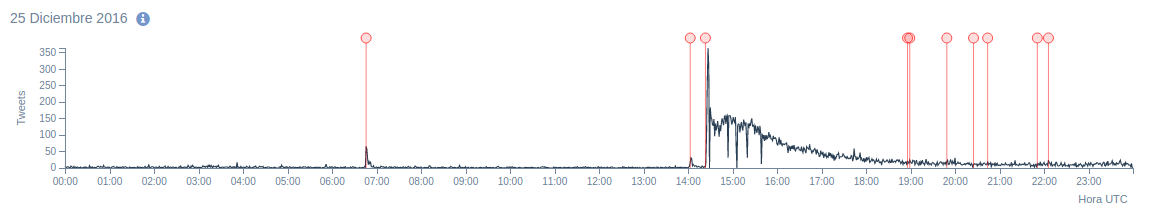
\includegraphics[width=\textwidth]{imagenes/img-25Dic-freq.png}
	  \caption{Frecuencia de mensajes relacionados con sismos durante el 25 de Diciembre del 2016.}
		\label{fig:timeline-25Dic}
	\end{figure}
	
	
	A las 14:24:30 hrs. del 25 de Diciembre del 2016 el sistema de detección basado en redes sociales detectó  un evento sísmico. La figura \ref{fig:timeline-25Dic} muestra la frecuencia de mensajes y el tercer marcador rojo, coincide con la detección antes mencionada. Los primeros \textit{tweets} publicados que mencionaban el suceso daban cuenta de que el sismo se percibía fuerte en Puerto Montt. A continuación se mencionan los 5 primeros mensajes publicados en la red social relacionados a este evento. 


\textit{``Temblor fuerte en Puerto mont'' $@$ginniasa, 14:23:27, 25/12/16}

\textit{``Está temblando heavy'' $@$loremba, 14:23:33 25/12/16}

\textit{``Dónde me duerma no me despierta ni un terremoto'' $@$SolRostan, 14:23:34 25/12/16}

\textit{``Temblando'' $@$fredyvargasr, 14:23:48 25/12/16}

\textit{``Temblor en \#puertomontt'' $@$correos73, 14:23:50 25/12/16}

	\begin{figure}[!ht]
	  \centering
	  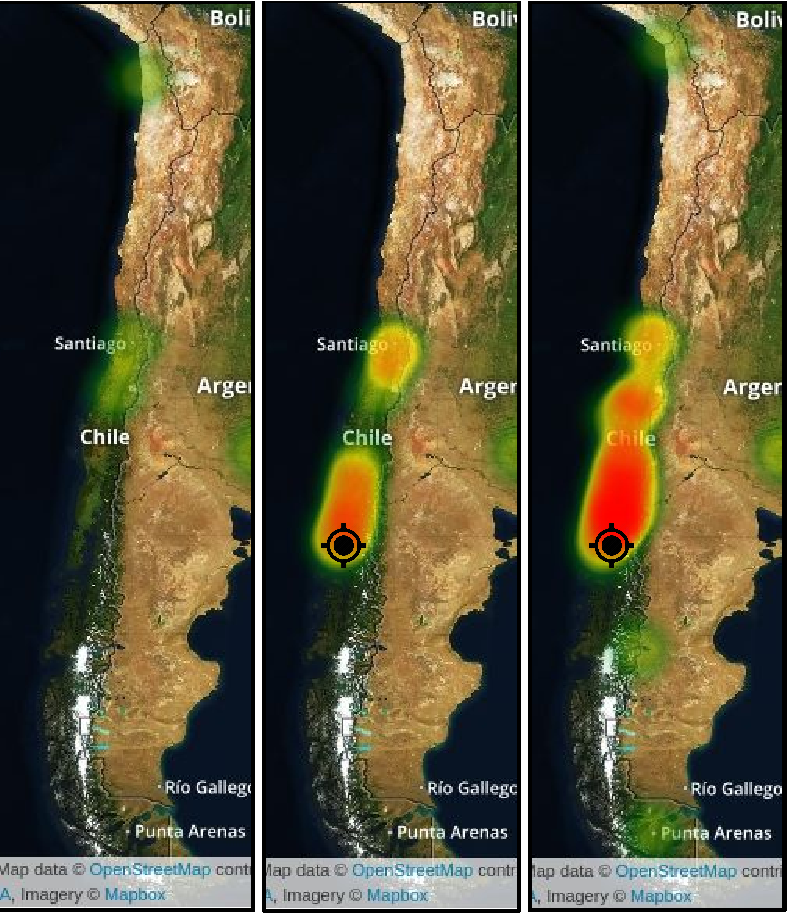
\includegraphics[trim={0 0 0 0}, clip, width=0.5\textwidth]{imagenes/heatmap.pdf}
	  \caption{Mapa de calor durante los primeros minutos posterior al inicio del sismo al norte de Melinka, Región de Aysén, Chile, el 25 de Diciembre del 2016.}
		\label{fig:heatmap-timelapse}
	\end{figure}	
	
	Durante el primer minuto posterior a la publicación del primer \textit{tweet} se publicaron 36 otros mensajes (sin contar \textit{retweets}). Además, luego de los primeros reportes, que generalmente son cortos y sin mucho detalle, se comienzan a compartir otros mensajes con información respecto a la intensidad del mismo. Mensajes cómo los presentados a continuación, ayudan a quien los lee, a entender que el sismo se percibió con una alta intensidad. 
	

\textit{``Hace mucho no sentía un temblor así'' $@$Estrella\_WTF, 14:26:00, 25/12/16}

\textit{``URGENTE Fuerte sismo se siente en \#Coyhaique'' $@$Radio45Sur, 14:26:00 25/12/16}

\textit{``Sendo temblor wn'' $@$goodzquad, 14:26:00 25/12/16}

\textit{``Fuerte temblor en el sur. Aquí en Purranque se sintió con tuti!!'' $@$Cristianc78, 14:26:00 25/12/16}

	\begin{figure}[!h]
	  \centering
	  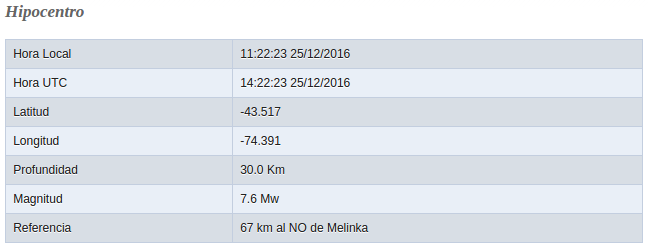
\includegraphics[trim={0 0 0 0}, clip, width=0.7\textwidth]{imagenes/img-25Dic-Hipocentro.png}
	  \caption{Vista de la aplicación Web disponible públicamente}
		\label{fig:25dic-hipocentro}
	\end{figure}
	
	La geolocalización de \textit{tweets} permitió presentar visualmente la zona en la cual las personas eran capaces de percibir movimiento. Las figuras \ref{fig:heatmap-timelapse} presentan la variación de las visualizaciones geográficas durante los primeros 5 minutos. En base a estas imágenes, es fácil inferir que el sismo fue percibido cerca de las regiones de Aysén y Los Ríos, ya que es en esa zona donde aparecen las primeras publicaciones. También se observa que al transcurrir los minutos, las personas comienzan a publicar mensajes desde zonas más alejadas. Esto se debe a dos razones principales, que la onda del sismo se percibe en diferentes instantes de tiempo dependiendo de la distancia focal y porque la noticia se difunde rápidamente a través de la red social. En este caso en particular, se observan mensajes en Santiago, sin embargo, el sismo fue percibido con muy baja intensidad en la Región Metropolitana, por lo que se infiere que esos \textit{tweets} corresponden a mensajes de difusión y que las personas no se encuentran necesariamente en el radio de percepción del sismo.
		
	La información oficial dispuesta por el Centro Sismológico Nacional (CSN) detalla que el epicentro del sismo se encuentra a 67 Km al Noroeste de Melinka, Región de Aysén, a 30 Km de profundidad y que la magnitud del sismo fue de 7,6 Mw. Lo que confirma lo inferido en base a las visualizaciones presentadas en la aplicación. La tabla de la figura \ref{fig:25dic-hipocentro} muestra otros detalles presentados por las fuentes oficiales. 
	Mientras este reporte fue publicado a pocos segundos del suceso, el informe preparado por la Oficina de Análisis en relación a la {\em intensidad}, es decir, el efecto que el sismo tuvo en la superficie y el alcance que tuvo en los pueblos de la zona, fue publicado a las 12:26 hrs. (4 minutos luego de ocurrido el suceso).
	Por lo tanto, previo a la entrega de este informe oficial, la aplicación ayudó a estimar de forma preliminar la gravedad de la situación. 
	
	
Cabe destacar que aunque el hipocentro de este sismo se ubicaba al norte de Melinka y en la zona sur de la isla de Chiloé, la mayoría de los \textit{tweets} fueron publicados por personas ubicadas al norte del hipocentro, cerca de la zona norte de la isla de Chiloé y también en Puerto Montt. Esto se puede explicar debido a la menor población de esas ciudades, acompañado de la heterogeneidad del uso de Twitter y del acceso a internet que existe a lo largo de las diferentes regiones de Chile.
	

	\section{Caso II: Sismos en otros países}
	
	El sistema propuesto está pensado para detectar sismos en diferentes idiomas y/o países. A continuación se presentan algunos casos de sismos ocurridos en otros países.  
	
	\subsection{Sismo en México}
	
\begin{figure}[!h]
	  \centering
	  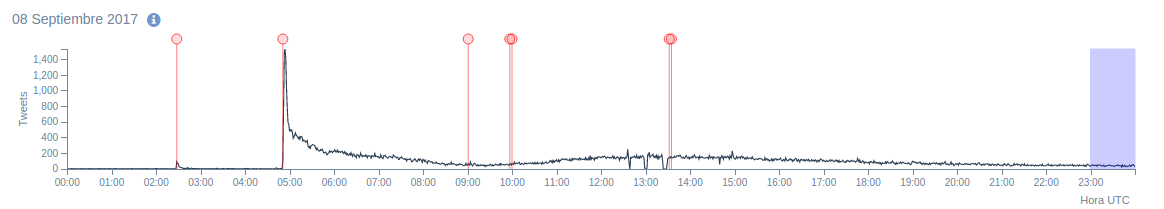
\includegraphics[width=\textwidth]{imagenes/img-sismo-mexico.png}
	  \caption{Frecuencia de mensajes relacionados con sismos durante el 8 de Septiembre del 2017.}
		\label{fig:timeline-mexico}
\end{figure}	
		
El terremoto de Chiapas de 2017 ocurrido 04:49:18, del jueves 8 de Septiembre (hora UTC). Tuvo una magnitud de 8,1 Mww, según el Servicio Geológico de los Estados Unidos (USGS)). El epicentro se ubicó en el Golfo de Tehuantepec, 137 km al suroeste de Pijijiapan (Chiapas), y a 69,7 km de profundidad. El sismo se percibió en el centro y sureste de México, así como en Guatemala, El Salvador, Honduras y Bélice.

	El sistema fue capaz de detectar este sismo sin problemas y debido a su gran intensidad se observó mucho ruido en la aplicación Web durante las horas posteriores al evento. La figura \ref{fig:timeline-mexico} muestra la frecuencia de mensajes el día 8 de Diciembre (Hora UTC). En las figuras \ref{fig:worldmap-mexico} y \ref{fig:worldmap-zoom-mexico} se puede observar cómo el sistema es capaz de informar acerca del lugar del evento y de otros lugares en los que este fue percibido. 
	
		\begin{figure}[!h]
\minipage{0.46\textwidth}
 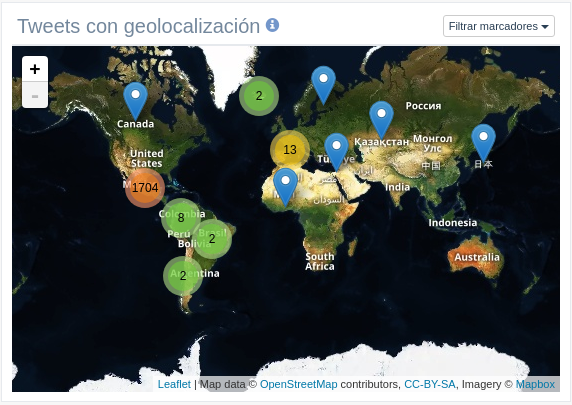
\includegraphics[width=\textwidth]{imagenes/img-worldmap-mexico.png}
	  \caption{Mapa del mundo con marcadores para los \textit{tweets} geolocalizados publicados durante los primeros minutos posteriores al inicio del sismo ocurrido en Chiapas, México en Semptiembre del 2017.}
		\label{fig:worldmap-mexico}
\endminipage\hfill
\minipage{0.46\textwidth}
 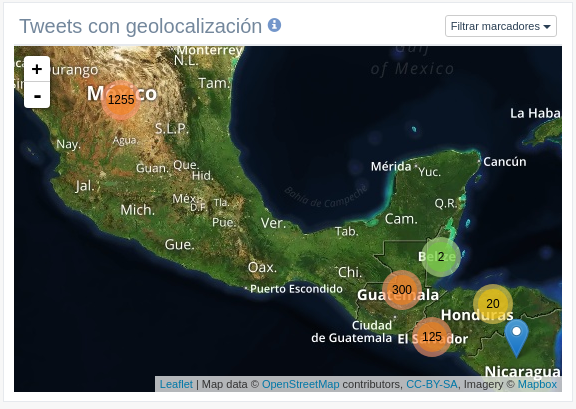
\includegraphics[trim={0 0 0 0}, clip, width=\textwidth]{imagenes/img-worldmap-zoom-mexico.png}
	  \caption{Mapa con marcadores para los \textit{tweets} geolocalizados, con zoom en la zona afectada,  publicados durante los primeros minutos posteriores al inicio del sismo ocurrido en Chiapas, México en Semptiembre del 2017.}
		\label{fig:worldmap-zoom-mexico}
\endminipage\hfill
\end{figure}
	
	\subsection{Sismo en Italia}
	
	\begin{figure}[!h]
	  \centering
	  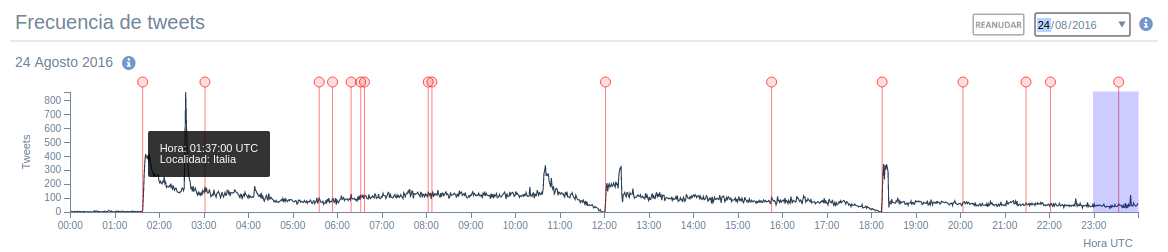
\includegraphics[width=\textwidth]{imagenes/sismoitaliafreq.png}
	  \caption{Frecuencia de mensajes relacionados con sismos durante el 24 de Agosto del 2016.}
		\label{fig:timeline-italia} 
	\end{figure}
	
	El día 24 de Agosto del 2016 a las 01:36 UTC, ocurrió un sismo muy fuerte en Italia central. Dada la magnitud del evento, el cual se registró con una magnitud de 6.2 Mw, el sistema fue capaz de detectarlo en menos de un minuto luego de la publicación del primer \textit{tweet}. Al observar la frecuencia de \textit{tweets} para ese día (figura \ref{fig:timeline-italia}), se observa una curva muy ruidosa y algunos picos que coinciden con los momentos importantes a lo largo del desarrollo de las actividades de recuperación. Muchos de los marcadores rojos dibujados a lo largo del día muestran momentos en los cuales hubo variaciones en la frecuencia, pero no necesariamente debido a un sismo, si no más bien, a puntos en donde se anunciaron los daños producidos. También hay depresiones abruptas en la frecuencia que se deben a las restricciones impuestas por Twitter debido al gran flujo de mensajes que se estaban recolectando. 
	
	El primer mensaje que hace alusión al sismo fue publicado a las 01:37 UTC y durante los primeros 5 minutos posteriores se publicaron aproximadamente 2000 \textit{tweets} que mencionan palabras clave relacionadas con sismos (sin contar \textit{retweets}). De estos, aproximadamente 885 mensajes fueron geolocalizados y en la figura \ref{fig:sismoitalia} se puede ver claramente que la mayoría de ellos fueron publicados desde Italia.
	
	\begin{figure}[!h]
	  \centering
	  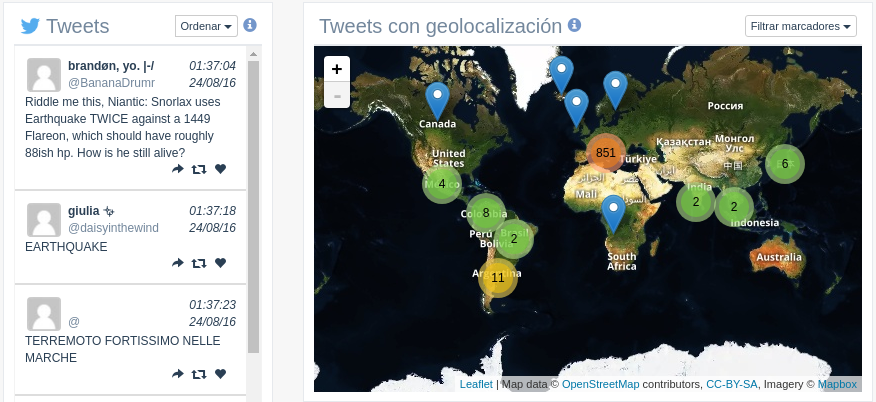
\includegraphics[width=\textwidth]{imagenes/sismoitalia.png}
	  \caption{Distribución de los mensajes publicados durante los primeros 10 minutos posterior al inicio del sismo en Italia central el 24 de Agosto del 2016.}
		\label{fig:sismoitalia}
	\end{figure}	
	
	La gravedad de la situación posterior al evento se reflejó en la red social, ya que durante el día, se continuaron publicando aproximadamente 100 mensajes por minuto haciendo referencia a sismos. Este comportamiento continuó hasta el día 25 de Agosto. Además, durante este periodo, los mensajes eran publicados desde diferentes países del mundo, demostrando ser un evento de interés internacional.
	
	
	\subsection{Otros Ejemplos}
	
	
	La figura \ref{fig:timeline-26Oct} muestra la frecuencia de \textit{tweets} del 26 de Octubre del 2016. Durante este día ocurrieron varios sismos en diferentes países y la herramienta fue capaz de detectarlos correctamente. 
	
	\begin{figure}[!h]
	  \centering
	  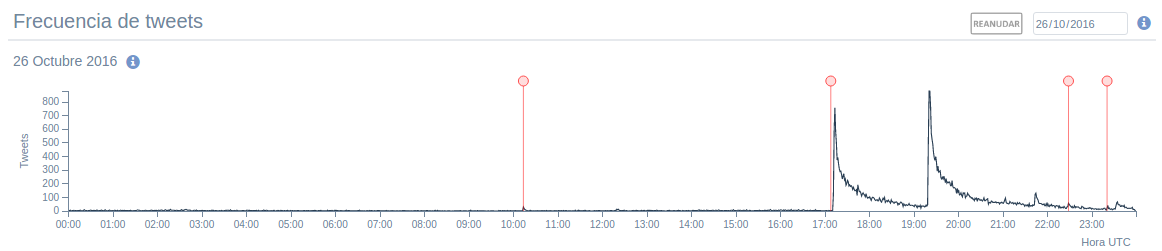
\includegraphics[width=\textwidth]{imagenes/26Octubrefreq.png}
	  \caption{Frecuencia de mensajes relacionados con sismos durante el 26 de Octubre del 2016.}
		\label{fig:timeline-26Oct}
	\end{figure}
	
	La primera detección que se visualiza en la aplicación Web ocurrió a las 10:13 UTC. Al seleccionar el rango de los 5 min posteriores se puede observar las visualización que se presenta en la imagen \ref{fig:sismojapon}. En la imagen se puede identificar que el evento ocurrió en Japón. La baja frecuencia asociada al evento se debe a que la aplicación Web muestra los datos filtrados por idiomas y este filtro no incluye el japonés, por lo que los \textit{tweets} visualizados corresponden únicamente a los escritos en inglés. 
	
	\begin{figure}[!h]
	  \centering
	  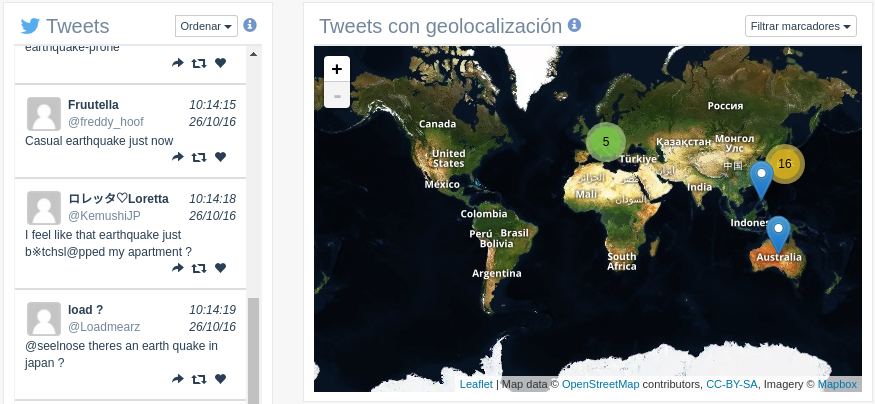
\includegraphics[width=\textwidth]{imagenes/sismoJapon.png}
	  \caption{Visualización de los mensajes publicados durante los primeros 5 minutos posterior al inicio de un sismo en Japón el 26 de Octubre del 2016.}
		\label{fig:sismojapon}
	\end{figure}
	
	
	La segunda detección ocurrida a las 17:07 UTC corresponde a un sismo en Italia y las ráfagas de \textit{tweets} que se observan a las 19:19 UTC y a las 21:43 UTC corresponden a otros sismos en Italia. En la visualización el segundo y tercer sismo no tienen marcadores. Este caso en el que sismos posteriores ocurridos en el mismo país no se marcan, se debe a que la velocidad de publicación de \textit{tweets} no alcanzó a decrecer lo suficiente antes de ocurrido el siguiente sismo y tampoco se mencionan nuevos países, por lo tanto se consideran como un mismo evento. 

	
	Al seleccionar los periodos de 5 min posterior a cada sismo se observa claramente el lugar donde ocurre el sismo y los tres eventos están ubicados en la península de Italia.
	
	\begin{figure}[ht]
	\centering
	\subfloat[Sismo detectado a las 17:07 UTC del 26 de Octubre del 2016.]{
		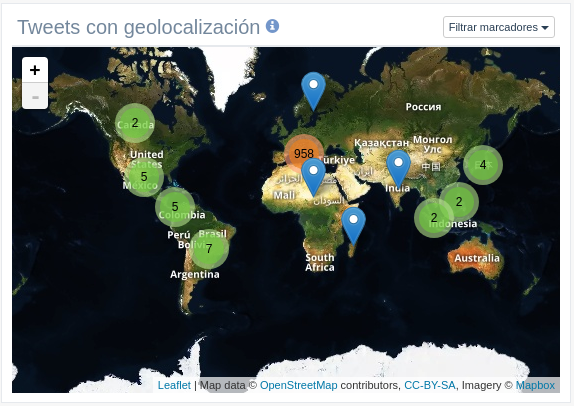
\includegraphics[width=140pt]{imagenes/sismoitalia-1.png}
		\label{fig:sismoitalia1}
	}
	\hfill
	\subfloat[Sismo detectado a las 19:19 UTC del 26 de Octubre del 2016.]{
  		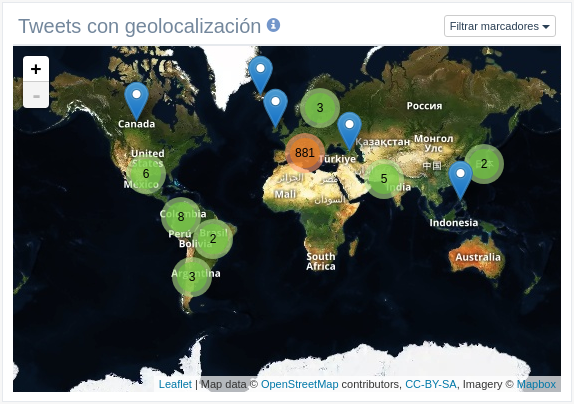
\includegraphics[width=140pt]{imagenes/sismoitalia-2.png}
  		\label{fig:sismoitalia2}
  	}
  	\hfill
	\subfloat[Sismo detectado a las 21;43 UTC del 26 de Octubre del 2016.]{
  		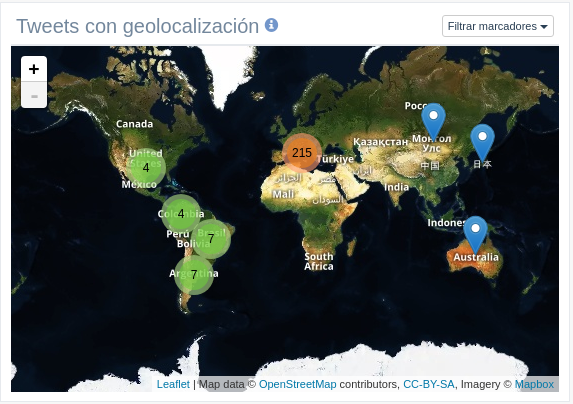
\includegraphics[width=140pt]{imagenes/sismoitalia-3.png}
  		\label{fig:sismoitalia3}
  	}
  	\caption{Distribución geográfica de los \textit{tweets} publicados en los 10 minutos posteriores a cada uno de los sismos detectados desde las 17:07 y las 21:43 del 26 de Octubre del 2016.}
  	\label{fig:sismoitaliamult}
  	\end{figure}
	
	La tercera detección ocurrida a las 22:28 UTC, se observa con una frecuencia muy baja. Al seleccionar el rango posterior a la detección se puede observar la distribución de los mensajes en el mapa y tal como se muestra en la imagen \ref{fig:sismocostarica-world}, aun existe una concentración importante de mensajes en Italia, pero también hay un grupo en la zona de América Central. Al acercar la imagen al sector de América Central \ref{fig:sismocostarica-zoom} se ve claramente que un sismo ha ocurrido en Costa Rica. 
	
	
	\begin{figure}[ht]
	\centering
	\subfloat[Mapa del mundo]{
		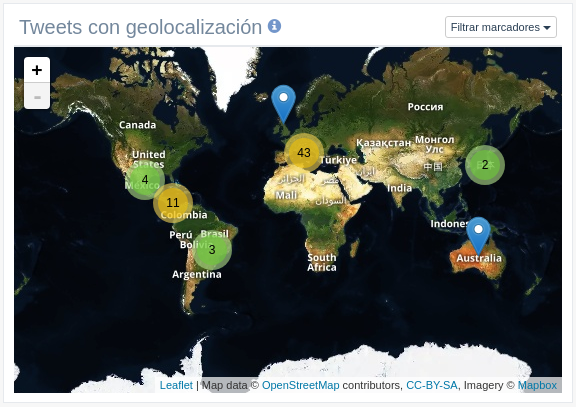
\includegraphics[width=220pt]{imagenes/sismocostarica1.png}
		\label{fig:sismocostarica-world}
	}
	\hfill
	\subfloat[Ampliación América Central]{
  		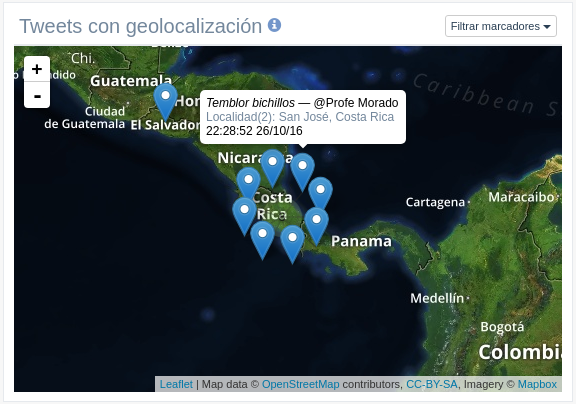
\includegraphics[width=220pt]{imagenes/sismocostarica.png}
  		\label{fig:sismocostarica-zoom}
  	}
  	\caption{Distribución de los \textit{tweets} publicados entre las 22:28 y las 22:38 UTC el 26 de Octubre del 2016.}
  	\label{fig:sismocostarica}
  	\end{figure}
	
	Finalmente, la última detección del día a las 23:20 UTC, tal como muestra la imagen \ref{fig:sismomexicoleve}, corresponde a un sismo en México. 
	
	\begin{figure}[!h]
	  \centering
	  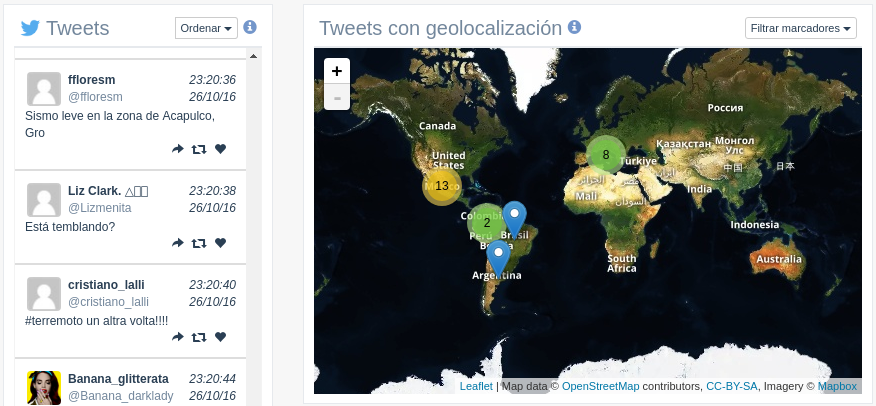
\includegraphics[width=\textwidth]{imagenes/sismomexicoleve.png}
	  \caption{Visualización de los mensajes publicados durante los primeros 5 minutos posterior al inicio de un sismo en México el 26 de Octubre del 2016.}
		\label{fig:sismomexicoleve}
	\end{figure}
	
	 
	\subsection{Observaciones}	 
	
	Para estos casos es interesante observar, que dependiendo del país en el que ocurre el sismo y de la intensidad de este, el ruido y el periodo de tiempo en el cual los usuarios de la red social continúan hablando del suceso puede variar desde un par de horas hasta incluso varios días.
	
	\section{Caso III: Falsos Positivos}
	\label{sec:casosfalsos}
	
	\begin{figure}[h]
	  \centering
	  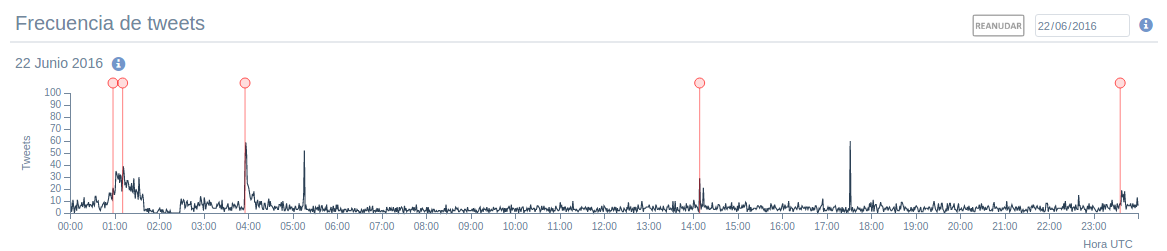
\includegraphics[trim={0 0 0 0}, clip, width=\textwidth]{imagenes/22junio2016-freq.png}
	  \caption{Frecuencia de mensajes relacionados con sismos durante el día 22 de Junio del 2016.}
		\label{fig:timeline-22junio}
	\end{figure}	
	
	Durante el periodo en el que el sistema ha estado disponible se han identificado algunos casos de detecciones falsas. El caso aquí presentado corresponde a un simulacro de sismo ocurrido en Filipinas el año 2016. Este simulacro, al ser de carácter masivo, ocasionó que muchas personas compartieran en la red social comentarios respectivos a su realización más o menos al mismo tiempo, de forma similar a como ocurre durante un evento sísmico real. En la imagen \ref{fig:timeline-22junio}, las dos primeras detecciones de ese día corresponden a falsos positivos. En este caso, la distribución de la frecuencia de \textit{tweets} es diferente a la que se observa durante un sismo real. Al seleccionar el rango de tiempo, se puede ver lo que se muestra en la figura \ref{fig:earthquakedrill}. En esta visualización se observa que los mensajes se geolocalizan en Filipinas por lo que se podría pensar que corresponde a un evento real, sin embargo, al revisar en detalle lo que dicen los mensajes, se menciona ``\textit{earthquake drill}'' lo que en español significa ``simulacro de terremoto''. 
	
	\begin{figure}[h]
	  \centering
	  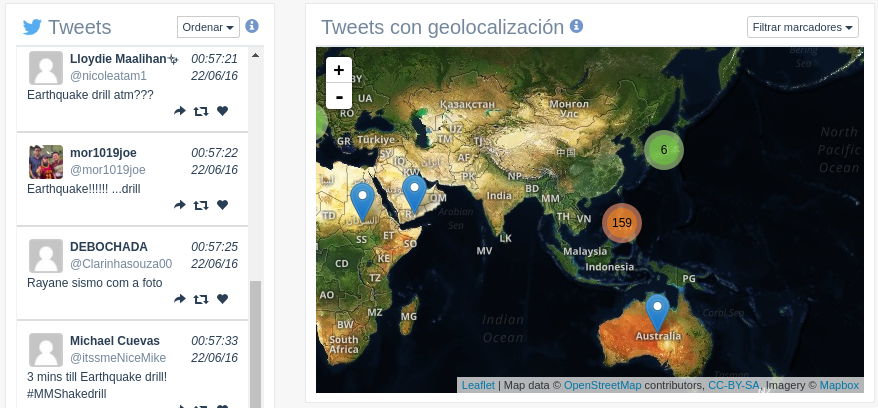
\includegraphics[width=\textwidth]{imagenes/earthquakedrill.png}
	  \caption{Visualización de los mensajes publicados entre las 00:45 y las 01:30 el 22 de Junio del 2016, durante un simulacro de sismo en Filipinas.}
		\label{fig:earthquakedrill}
	\end{figure}	
	
	A pesar de que se identificaron casos de ese tipo, al presentar características muy similares a las de un sismo real, no se tomaron medidas para filtrarlos. Sin embargo, gracias a la disposición de los elementos en la aplicación Web, se puede identificar fácilmente, mediante la lectura de algunos de los mensajes publicados, que no se trata de un sismo real, si no más bien de un simulacro masivo. 
	
	
\begin{conclusion}
\label{cap:conclusion}	

Se ha presentado un enfoque simple y eficiente para la detección de sismos basada en sensores sociales. El enfoque propuesto difiere de otros trabajos existentes en que es un modelo no supervisado y tolerante al ruido de los mensajes, permitiendo de esta forma, monitorizar eventos en todo el mundo y en diferentes idiomas. La parametrización inicial es de bajo costo, ya que no necesita conjuntos de mensajes etiquetados ni procesos de entrenamiento. Además, se adapta automáticamente en el tiempo dependiendo de las variaciones en la velocidad de llegada de los mensajes de interés. Los experimentos realizados muestran que el algoritmo propuesto es competitivo en relación al estado del arte, mejorando tanto la precisión como el {\em recall}. Al ser tolerante al ruido, es capaz de retener un número mayor de mensajes sin afectar la detección, los que son utilizados para la descripción de los eventos. Al tener más mensajes es posible describir los eventos de forma más detallada y diferenciar, por ejemplo, cuando ocurren dos eventos consecutivos en lugares diferentes. Esto contribuye a crear catálogos más completos. El enfoque de detección de sismos en base a sensores sociales está limitado por la cobertura geográfica de Twitter y por lo tanto no será posible detectar sismos rápidamente en áreas que no estén habitadas por usuarios de Twitter. 

Por otro lado, se desarrolló una aplicación Web que despliega la información obtenida en tiempo real. Esta aplicación es utilizada por el Centro Sismológico Nacional de la Universidad de Chile (CSN) y por el Servicio Hidrográfico y Oceanográfico de la Armada de Chile (SHOA) para complementar sus fuentes de información durante eventos sísmicos. 
% Aqui mencionar la utilidad en casos especificos de los casos de estudio presentados.
La aplicación también permite explorar los datos históricos de eventos sísmicos pasados, disponibles desde la fecha en que se puso el marcha el sistema recolector de información (Octubre 2015). Las visualizaciones disponibles en la aplicación están orientadas para que los usuarios del sistema puedan responder rápidamente a tres preguntas, las que ayudan a entender, de forma general, un evento. Las preguntas son: 
\begin{enumerate}
\item ¿Qué sucedió? Esta pregunta se puede responder observando los mensajes publicados por las personas en relación al sismo.
\item ¿Cuándo sucedió? La línea tiempo que muestra la frecuencia de los mensajes permite observar rápidamente el momento en el cual comienza el evento. 
\item ¿Dónde sucedió? Los mapas de calor y de marcadores permiten identificar la zona afectada. Además, durante los minutos posteriores a cada evento, permiten observar cómo la noticia se difunde hacia otras partes del mundo.
\end{enumerate} 

Además, durante el periodo de desarrollo de esta tesis se aceptó una publicación sobre el sistema de detección de sismos propuesto y su evaluación en \textit{The 5th AAAI Conference on Human Computation and Crowdsourcing} (HCOMP 2017). El artículo aceptado se encuentra disponible en los anexos. Previamente, también se había enviado una versión más corta a la conferencia \textit{The 40th International ACM SIGIR Conference on Research and Development in Information Retrieval} (SIGIR 2017) el cual lamentablemente no fue aceptado debido a que las mejoras del sistema propuesto con respecto al estado del arte no fueron expuestas de forma que los evaluadores las consideraran lo suficientemente relevantes. Este primer intento y las revisiones de los evaluadores permitieron preparar una versión más clara y completa.

Cómo se mencionó previamente, la información recolectada hasta la fecha se ha almacenado para estudios y trabajos futuros. Dentro de los posibles estudios a realizar usando los datos de sensores sociales se encuentran: la estimación del tamaño de un sismo, la estimación de la intensidad en diferentes zonas geográficas, la generalización del sistema para su uso en detección de otros tipos de catástrofes naturales que afectan a las ciudades de Chile (erupciones, maremotos, incendios, etc), entre otros.

\end{conclusion}



\bibliographystyle{plain}
\phantomsection
\addcontentsline{toc}{chapter}{Bibliografía}
\bibliography{bibliografia}

\phantomsection
\addcontentsline{toc}{chapter}{Anexo A: Evaluación por País del Sistema de Detección de Sismos}
\chapter*{Anexo I: Evaluación por País del Sistema de Detección de Sismos}
\label{anexo:evaluacionpaises}

{\small
\begin{table}[!ht]
\centering
  \begin{tabular}{|l|ccc|c|ccc|}
  \hline
  País - Estado & TP & TN & FN & USGS reports & P & R & F-M \\
  \hline \hline
Indonesia	 & 838 	 & 308 	 & 40 	& 1146	 & 0,95 &	0,73 &	0,83 \\ \hline
Japan	 & 582 	 & 172 	 & 12 	& 754	 & 0,98 &	0,77 &	0,86 \\ \hline
USA - Alaska	 & 576 	 & 1865 	 & 326 	& 2441	 & 0,64 &	0,24 &	0,34 \\ \hline
New Zealand	 & 446 	 & 112 	 & 21 	& 558	 & 0,96 &	0,80 &	0,87 \\ \hline
Chile	 & 377 	 & 151 	 & 29 	& 528	 & 0,93 &	0,71 &	0,81 \\ \hline
Papua New Guinea	 & 345 	 & 132 	 & 19 	& 477	 & 0,95 &	0,72 &	0,82 \\ \hline
Fiji	 & 339 	 & 108 	 & 30 	& 447	 & 0,92 &	0,76 &	0,83 \\ \hline
Vanuatu	 & 308 	 & 116 	 & 24 	& 424	 & 0,93 &	0,73 &	0,81 \\ \hline
Philippines	 & 276 	 & 102 	 & 8 	& 378	 & 0,97 &	0,73 &	0,83 \\ \hline
Tonga	 & 225 	 & 83 	 & 14 	& 308	 & 0,94 &	0,73 &	0,82 \\ \hline
Northern Mariana Islands	 & 209 	 & 74 	 & 25 	& 283	 & 0,89 &	0,74 &	0,81 \\ \hline
\begin{tabular}{@{}l@{}} South Georgia and the South \\ Sandwich Islands \end{tabular}	 & 204 	 & 56 	 & 7 	& 260	 & 0,97 &	0,78 &	0,87 \\ \hline
USA - Oklahoma	 & 193 	 & 996 	 & 129 	& 1189	 & 0,60 &	0,16 &	0,26 \\ \hline
Russia	 & 175 	 & 69 	 & 6 	& 244	 & 0,97 &	0,72 &	0,82 \\ \hline
Mexico	 & 163 	 & 77 	 & 14 	& 240	 & 0,92 &	0,68 &	0,78 \\ \hline
South of the Fiji Islands	 & 141 	 & 53 	 & 15 	& 194	 & 0,90 &	0,73 &	0,81 \\ \hline
Peru	 & 136 	 & 45 	 & 0   	& 181	 & 1,00 &	0,75 &	0,86 \\ \hline
Solomon Islands	 & 119 	 & 40 	 & 5 	& 159	 & 0,96 &	0,75 &	0,84 \\ \hline
Puerto Rico	 & 116 	 & 523 	 & 51 	& 639	 & 0,69 &	0,18 &	0,29 \\ \hline
Southwest Indian Ridge	 & 110 	 & 21 	 & 3 	& 131	 & 0,97 &	0,84 &	0,90 \\ \hline
China	 & 104 	 & 40 	 & 0   	& 144	 & 1,00 &	0,72 &	0,84 \\ \hline
USA - California	 & 100 	 & 381 	 & 47 	& 481	 & 0,68 &	0,21 &	0,32 \\ \hline
Argentina	 & 99 	 & 35 	 & 6 	& 134	 & 0,94 &	0,74 &	0,83 \\ \hline
   \end{tabular}
  \caption{Evaluación de detecciones por país realizadas utilizando el sistema basado en sensores sociales y considerando el catálogo de sismos del USGS.}
  \label{table:all-detections-01}
\end{table}}

{\small
\begin{table}[!ht]
\centering
  \begin{tabular}{|l|ccc|c|ccc|}
  \hline
  País - Estado & TP & TN & FN & USGS reports & P & R & F-M \\
  \hline \hline
Ecuador	 & 98 	 & 47 	 & 8 	& 145	 & 0,92 &	0,68 &	0,78 \\ \hline
Afghanistan	 & 95 	 & 33 	 & 8 	& 128	 & 0,92 &	0,74 &	0,82 \\ \hline
New Caledonia	 & 89 	 & 33 	 & 5 	& 122	 & 0,95 &	0,73 &	0,82 \\ \hline
Greece	 & 83 	 & 30 	 & 5 	& 113	 & 0,94 &	0,73 &	0,83 \\ \hline
South Georgia Island region	 & 80 	 & 19 	 & 2 	& 99	 & 0,98 &	0,81 &	0,88 \\ \hline
British Virgin Islands	 & 74 	 & 260 	 & 41 	& 334	 & 0,64 &	0,22 &	0,33 \\ \hline
Tajikistan	 & 59 	 & 13 	 & 4 	& 72	 & 0,94 &	0,82 &	0,87 \\ \hline
Nicaragua	 & 58 	 & 15 	 & 6 	& 73	 & 0,91 &	0,79 &	0,85 \\ \hline
Kyrgyzstan	 & 56 	 & 11 	 & 3 	& 67	 & 0,95 &	0,84 &	0,89 \\ \hline
Guam	 & 55 	 & 25 	 & 3 	& 80	 & 0,95 &	0,69 &	0,80 \\ \hline
Taiwan	 & 52 	 & 17 	 & 1 	& 69	 & 0,98 &	0,75 &	0,85 \\ \hline
Guatemala	 & 51 	 & 15 	 & 3 	& 66	 & 0,94 &	0,77 &	0,85 \\ \hline
Colombia	 & 48 	 & 12 	 & 7 	& 60	 & 0,87 &	0,80 &	0,83 \\ \hline
Iran	 & 47 	 & 20 	 & 0   	& 67	 & 1,00 &	0,70 &	0,82 \\ \hline
India	 & 47 	 & 18 	 & 2 	& 65	 & 0,96 &	0,72 &	0,82 \\ \hline
El Salvador	 & 46 	 & 21 	 & 4 	& 67	 & 0,92 &	0,69 &	0,79 \\ \hline
Northern Mid-Atlantic Ridge	 & 46 	 & 10 	 & 3 	& 56	 & 0,94 &	0,82 &	0,88 \\ \hline
Central Mid-Atlantic Ridge	 & 43 	 & 20 	 & 0   	& 63	 & 1,00 &	0,68 &	0,81 \\ \hline
Micronesia	 & 41 	 & 6 	 & 0   	& 47	 & 1,00 &	0,87 &	0,93 \\ \hline
East Timor	 & 40 	 & 18 	 & 1 	& 58	 & 0,98 &	0,69 &	0,81 \\ \hline
South Sandwich Islands	 & 37 	 & 11 	 & 1 	& 48	 & 0,97 &	0,77 &	0,86 \\ \hline
Reykjanes Ridge	 & 32 	 & 12 	 & 2 	& 44	 & 0,94 &	0,73 &	0,82 \\ \hline
Dominican Republic	 & 31 	 & 104 	 & 25 	& 135	 & 0,55 &	0,23 &	0,32 \\ \hline
southern Mid-Atlantic Ridge	 & 31 	 & 14 	 & 2 	& 45	 & 0,94 &	0,69 &	0,79 \\ \hline
USA - Hawaii	 & 28 	 & 114 	 & 20 	& 142	 & 0,58 &	0,20 &	0,29 \\ \hline
Morocco	 & 28 	 & 13 	 & 0   	& 41	 & 1,00 &	0,68 &	0,81 \\ \hline
Pakistan	 & 27 	 & 3 	 & 1 	& 30	 & 0,96 &	0,90 &	0,93 \\ \hline
Italy	 & 27 	 & 3 	 & 0   	& 30	 & 1,00 &	0,90 &	0,95 \\ \hline
Canada	 & 25 	 & 66 	 & 9 	& 91	 & 0,74 &	0,27 &	0,40 \\ \hline
Kuril Islands	 & 25 	 & 5 	 & 0   	& 30	 & 1,00 &	0,83 &	0,91 \\ \hline
Turkey	 & 25 	 & 4 	 & 1 	& 29	 & 0,96 &	0,86 &	0,91 \\ \hline
Japan region	 & 23 	 & 6 	 & 0   	& 29	 & 1,00 &	0,79 &	0,88 \\ \hline
Mid-Indian Ridge	 & 22 	 & 9 	 & 0   	& 31	 & 1,00 &	0,71 &	0,83 \\ \hline
Burma	 & 22 	 & 4 	 & 3 	& 26	 & 0,88 &	0,85 &	0,86 \\ \hline
South Indian Ocean	 & 22 	 & 2 	 & 1 	& 24	 & 0,96 &	0,92 &	0,94 \\ \hline
Australia	 & 20 	 & 6 	 & 2 	& 26	 & 0,91 &	0,77 &	0,83 \\ \hline
North of Ascension Island	 & 20 	 & 6 	 & 2 	& 26	 & 0,91 &	0,77 &	0,83 \\ \hline
US Virgin Islands	 & 19 	 & 84 	 & 28 	& 103	 & 0,40 &	0,18 &	0,25 \\ \hline
Southern East Pacific Rise	 & 19 	 & 10 	 & 0   	& 29	 & 1,00 &	0,66 &	0,79 \\ \hline
Bolivia	 & 18 	 & 13 	 & 2 	& 31	 & 0,90 &	0,58 &	0,71 \\ \hline
central East Pacific Rise	 & 18 	 & 4 	 & 0   	& 22	 & 1,00 &	0,82 &	0,90 \\ \hline
Wallis and Futuna	 & 18 	 & 4 	 & 0   	& 22	 & 1,00 &	0,82 &	0,90 \\ \hline
   \end{tabular}
  \caption{Evaluación de detecciones por país realizadas utilizando el sistema basado en sensores sociales y considerando el catálogo de sismos del USGS.}
  \label{table:all-detections-02}
\end{table}}

{\small
\begin{table}[!ht]
\centering
  \begin{tabular}{|l|ccc|c|ccc|}
  \hline
  País - Estado & TP & TN & FN & USGS reports & P & R & F-M \\
  \hline \hline
Pacific-Antarctic Ridge	 & 16 	 & 8 	 & 2 	& 24	 & 0,89 &	0,67 &	0,76 \\ \hline
Nepal	 & 15 	 & 6 	 & 0   	& 21	 & 1,00 &	0,71 &	0,83 \\ \hline
Balleny Islands region	 & 14 	 & 6 	 & 5 	& 20	 & 0,74 &	0,70 &	0,72 \\ \hline
Costa Rica	 & 14 	 & 6 	 & 2 	& 20	 & 0,88 &	0,70 &	0,78 \\ \hline
Carlsberg Ridge	 & 14 	 & 4 	 & 0   	& 18	 & 1,00 &	0,78 &	0,88 \\ \hline
Portugal	 & 14 	 & 3 	 & 0   	& 17	 & 1,00 &	0,82 &	0,90 \\ \hline
USA - Nevada	 & 13 	 & 63 	 & 9 	& 76	 & 0,59 &	0,17 &	0,27 \\ \hline
Panama	 & 13 	 & 6 	 & 1 	& 19	 & 0,93 &	0,68 &	0,79 \\ \hline
South of the Kermadec Islands	 & 13 	 & 3 	 & 1 	& 16	 & 0,93 &	0,81 &	0,87 \\ \hline
Venezuela	 & 13 	 & 0   	 & 2 	& 13	 & 0,87 &	1,00 &	0,93 \\ \hline
Western Indian-Antarctic Ridge	 & 12 	 & 10 	 & 2 	& 22	 & 0,86 &	0,55 &	0,67 \\ \hline
Yemen	 & 12 	 & 3 	 & 0   	& 15	 & 1,00 &	0,80 &	0,89 \\ \hline
East of the Kuril Islands	 & 12 	 & 1 	 & 2 	& 13	 & 0,86 &	0,92 &	0,89 \\ \hline
USA - Oregon	 & 10 	 & 37 	 & 5 	& 47	 & 0,67 &	0,21 &	0,32 \\ \hline
West of Macquarie Island	 & 10 	 & 7 	 & 0   	& 17	 & 1,00 &	0,59 &	0,74 \\ \hline
Svalbard and Jan Mayen	 & 10 	 & 4 	 & 2 	& 14	 & 0,83 &	0,71 &	0,77 \\ \hline
Southeast of Easter Island	 & 9 	 & 6 	 & 0   	& 15	 & 1,00 &	0,60 &	0,75 \\ \hline
South of Africa	 & 9 	 & 4 	 & 2 	& 13	 & 0,82 &	0,69 &	0,75 \\ \hline
Vanuatu region	 & 9 	 & 2 	 & 0   	& 11	 & 1,00 &	0,82 &	0,90 \\ \hline
South Sandwich Islands region	 & 9 	 & 1 	 & 0   	& 10	 & 1,00 &	0,90 &	0,95 \\ \hline
Southwest of Africa	 & 9 	 & 1 	 & 0   	& 10	 & 1,00 &	0,90 &	0,95 \\ \hline
Honduras	 & 8 	 & 2 	 & 0   	& 10	 & 1,00 &	0,80 &	0,89 \\ \hline
Guadeloupe	 & 8 	 & 0   	 & 2 	& 8	 & 0,80 &	1,00 &	0,89 \\ \hline
South of Panama	 & 8 	 & 0   	 & 1 	& 8	 & 0,89 &	1,00 &	0,94 \\ \hline
USA - Kansas	 & 7 	 & 55 	 & 5 	& 62	 & 0,58 &	0,11 &	0,19 \\ \hline
Southeast Indian Ridge	 & 7 	 & 5 	 & 0   	& 12	 & 1,00 &	0,58 &	0,74 \\ \hline
Macedonia	 & 7 	 & 3 	 & 2 	& 10	 & 0,78 &	0,70 &	0,74 \\ \hline
Algeria	 & 7 	 & 2 	 & 0   	& 9	 & 1,00 &	0,78 &	0,88 \\ \hline
South Africa	 & 7 	 & 1 	 & 1 	& 8	 & 0,88 &	0,88 &	0,88 \\ \hline
Indian Ocean Triple Junction	 & 7 	 & 1 	 & 0   	& 8	 & 1,00 &	0,88 &	0,93 \\ \hline
Northern East Pacific Rise	 & 6 	 & 6 	 & 0   	& 12	 & 1,00 &	0,50 &	0,67 \\ \hline
Saint Helena	 & 6 	 & 1 	 & 0   	& 7	 & 1,00 &	0,86 &	0,92 \\ \hline
Saudi Arabia	 & 6 	 & 1 	 & 0   	& 7	 & 1,00 &	0,86 &	0,92 \\ \hline
Ascension Island region	 & 6 	 & 0   	 & 0   	& 6	 & 1,00 &	1,00 &	1,00 \\ \hline
Off the coast of Oregon	 & 5 	 & 17 	 & 2 	& 22	 & 0,71 &	0,23 &	0,34 \\ \hline
Off the west coast of northern Sumatra	 & 5 	 & 8 	 & 0   	& 13	 & 1,00 &	0,38 &	0,56 \\ \hline
West Chile Rise	 & 5 	 & 6 	 & 0   	& 11	 & 1,00 &	0,45 &	0,63 \\ \hline
Chagos Archipelago region	 & 5 	 & 5 	 & 2 	& 10	 & 0,71 &	0,50 &	0,59 \\ \hline
Prince Edward Islands region	 & 5 	 & 4 	 & 0   	& 9	 & 1,00 &	0,56 &	0,71 \\ \hline
Banda Sea	 & 5 	 & 3 	 & 0   	& 8	 & 1,00 &	0,63 &	0,77 \\ \hline
Easter Island region	 & 5 	 & 2 	 & 2 	& 7	 & 0,71 &	0,71 &	0,71 \\ \hline
Greenland	 & 5 	 & 2 	 & 0   	& 7	 & 1,00 &	0,71 &	0,83 \\ \hline
   \end{tabular}
  \caption{Evaluación de detecciones por país realizadas utilizando el sistema basado en sensores sociales y considerando el catálogo de sismos del USGS.}
  \label{table:all-detections-03}
\end{table}}

{\small
\begin{table}[!ht]
\centering
  \begin{tabular}{|l|ccc|c|ccc|}
  \hline
  País - Estado & TP & TN & FN & USGS reports & P & R & F-M \\
  \hline \hline
South of Tonga	 & 5 	 & 2 	 & 0   	& 7	 & 1,00 &	0,71 &	0,83 \\ \hline
Cyprus	 & 5 	 & 1 	 & 0   	& 6	 & 1,00 &	0,83 &	0,91 \\ \hline
Antarctica	 & 5 	 & 0   	 & 0   	& 5	 & 1,00 &	1,00 &	1,00 \\ \hline
USA - Montana	 & 4 	 & 20 	 & 3 	& 24	 & 0,57 &	0,17 &	0,26 \\ \hline
USA - Wyoming	 & 4 	 & 8 	 & 1 	& 12	 & 0,80 &	0,33 &	0,47 \\ \hline
France	 & 4 	 & 6 	 & 0   	& 10	 & 1,00 &	0,40 &	0,57 \\ \hline
Bouvet Island	 & 4 	 & 3 	 & 2 	& 7	 & 0,67 &	0,57 &	0,62 \\ \hline
Tanzania	 & 4 	 & 3 	 & 1 	& 7	 & 0,80 &	0,57 &	0,67 \\ \hline
USA - Tennessee	 & 4 	 & 3 	 & 0   	& 7	 & 1,00 &	0,57 &	0,73 \\ \hline
North Atlantic Ocean	 & 4 	 & 2 	 & 0   	& 6	 & 1,00 &	0,67 &	0,80 \\ \hline
North of Svalbard	 & 4 	 & 2 	 & 0   	& 6	 & 1,00 &	0,67 &	0,80 \\ \hline
Uzbekistan	 & 4 	 & 2 	 & 0   	& 6	 & 1,00 &	0,67 &	0,80 \\ \hline
Barbuda	 & 4 	 & 1 	 & 0   	& 5	 & 1,00 &	0,80 &	0,89 \\ \hline
Dominica	 & 4 	 & 1 	 & 0   	& 5	 & 1,00 &	0,80 &	0,89 \\ \hline
Somalia	 & 4 	 & 1 	 & 0   	& 5	 & 1,00 &	0,80 &	0,89 \\ \hline
Western Xizang	 & 4 	 & 1 	 & 0   	& 5	 & 1,00 &	0,80 &	0,89 \\ \hline
Mauritius	 & 4 	 & 0   	 & 1 	& 4	 & 0,80 &	1,00 &	0,89 \\ \hline
\begin{tabular}{@{}l@{}} Off the east coast of the \\ North Island of New Zealand \end{tabular}	 & 4 	 & 0   	 & 1 	& 4	 & 0,80 &	1,00 &	0,89 \\ \hline
Albania	 & 4 	 & 0   	 & 0   	& 4	 & 1,00 &	1,00 &	1,00 \\ \hline
Cuba	 & 4 	 & 0   	 & 0   	& 4	 & 1,00 &	1,00 &	1,00 \\ \hline
Martinique	 & 4 	 & 0   	 & 0   	& 4	 & 1,00 &	1,00 &	1,00 \\ \hline
Owen Fracture Zone region	 & 4 	 & 0   	 & 0   	& 4	 & 1,00 &	1,00 &	1,00 \\ \hline
Timor Sea	 & 4 	 & 0   	 & 0   	& 4	 & 1,00 &	1,00 &	1,00 \\ \hline
USA - Texas	 & 3 	 & 6 	 & 2 	& 9	 & 0,60 &	0,33 &	0,43 \\ \hline
Scotia Sea	 & 3 	 & 4 	 & 7 	& 7	 & 0,30 &	0,43 &	0,35 \\ \hline
Off the coast of Central America	 & 3 	 & 4 	 & 0   	& 7	 & 1,00 &	0,43 &	0,60 \\ \hline
North of Severnaya Zemlya	 & 3 	 & 2 	 & 0   	& 5	 & 1,00 &	0,60 &	0,75 \\ \hline
South Korea	 & 3 	 & 2 	 & 0   	& 5	 & 1,00 &	0,60 &	0,75 \\ \hline
Poland	 & 3 	 & 1 	 & 1 	& 4	 & 0,75 &	0,75 &	0,75 \\ \hline
Azerbaijan	 & 3 	 & 1 	 & 0   	& 4	 & 1,00 &	0,75 &	0,86 \\ \hline
Christmas Island	 & 3 	 & 1 	 & 0   	& 4	 & 1,00 &	0,75 &	0,86 \\ \hline
Kazakhstan	 & 3 	 & 1 	 & 0   	& 4	 & 1,00 &	0,75 &	0,86 \\ \hline
USA - Georgia	 & 3 	 & 0   	 & 1 	& 3	 & 0,75 &	1,00 &	0,86 \\ \hline
Democratic Republic of the Congo	 & 3 	 & 0   	 & 0   	& 3	 & 1,00 &	1,00 &	1,00 \\ \hline
Prince Edward Islands	 & 3 	 & 0   	 & 0   	& 3	 & 1,00 &	1,00 &	1,00 \\ \hline
USA - Utah	 & 2 	 & 12 	 & 0   	& 14	 & 1,00 &	0,14 &	0,25 \\ \hline
USA - Missouri	 & 2 	 & 5 	 & 4 	& 7	 & 0,33 &	0,29 &	0,31 \\ \hline
Anguilla	 & 2 	 & 5 	 & 1 	& 7	 & 0,67 &	0,29 &	0,40 \\ \hline
USA - Colorado	 & 2 	 & 5 	 & 0   	& 7	 & 1,00 &	0,29 &	0,44 \\ \hline
South of Australia	 & 2 	 & 4 	 & 0   	& 6	 & 1,00 &	0,33 &	0,50 \\ \hline
Samoa	 & 2 	 & 3 	 & 0   	& 5	 & 1,00 &	0,40 &	0,57 \\ \hline
   \end{tabular}
  \caption{Evaluación de detecciones por país realizadas utilizando el sistema basado en sensores sociales y considerando el catálogo de sismos del USGS.}
  \label{table:all-detections-04}
\end{table}}

{\small
\begin{table}[!ht]
\centering
  \begin{tabular}{|l|ccc|c|ccc|}
  \hline
  País - Estado & TP & TN & FN & USGS reports & P & R & F-M \\
  \hline \hline
North Indian Ocean	 & 2 	 & 2 	 & 0   	& 4	 & 1,00 &	0,50 &	0,67 \\ \hline
Zimbabwe	 & 2 	 & 2 	 & 0   	& 4	 & 1,00 &	0,50 &	0,67 \\ \hline
Iraq	 & 2 	 & 1 	 & 1 	& 3	 & 0,67 &	0,67 &	0,67 \\ \hline
Croatia	 & 2 	 & 1 	 & 0   	& 3	 & 1,00 &	0,67 &	0,80 \\ \hline
Iceland	 & 2 	 & 1 	 & 0   	& 3	 & 1,00 &	0,67 &	0,80 \\ \hline
Romania	 & 2 	 & 1 	 & 0   	& 3	 & 1,00 &	0,67 &	0,80 \\ \hline
South Shetland Islands	 & 2 	 & 1 	 & 0   	& 3	 & 1,00 &	0,67 &	0,80 \\ \hline
Spain	 & 2 	 & 1 	 & 0   	& 3	 & 1,00 &	0,67 &	0,80 \\ \hline
Tristan da Cunha region	 & 2 	 & 1 	 & 0   	& 3	 & 1,00 &	0,67 &	0,80 \\ \hline
Azores Islands region	 & 2 	 & 0   	 & 0   	& 2	 & 1,00 &	1,00 &	1,00 \\ \hline
Bangladesh	 & 2 	 & 0   	 & 0   	& 2	 & 1,00 &	1,00 &	1,00 \\ \hline
\begin{tabular}{@{}l@{}} East of the North Island\\ of New Zealand \end{tabular} & 2 	 & 0   	 & 0   	& 2	 & 1,00 &	1,00 &	1,00 \\ \hline
Greenland Sea	 & 2 	 & 0   	 & 0   	& 2	 & 1,00 &	1,00 &	1,00 \\ \hline
Macquarie Island region	 & 2 	 & 0   	 & 0   	& 2	 & 1,00 &	1,00 &	1,00 \\ \hline
Mariana Islands region	 & 2 	 & 0   	 & 0   	& 2	 & 1,00 &	1,00 &	1,00 \\ \hline
Switzerland	 & 2 	 & 0   	 & 0   	& 2	 & 1,00 &	1,00 &	1,00 \\ \hline
Syria	 & 2 	 & 0   	 & 0   	& 2	 & 1,00 &	1,00 &	1,00 \\ \hline
Turkmenistan	 & 2 	 & 0   	 & 0   	& 2	 & 1,00 &	1,00 &	1,00 \\ \hline
West of the Galapagos Islands	 & 2 	 & 0   	 & 0   	& 2	 & 1,00 &	1,00 &	1,00 \\ \hline
USA - Washington	 & 1 	 & 16 	 & 12 	& 17	 & 0,08 &	0,06 &	0,07 \\ \hline
USA - Idaho	 & 1 	 & 12 	 & 1 	& 13	 & 0,50 &	0,08 &	0,13 \\ \hline
USA - Arizona	 & 1 	 & 4 	 & 1 	& 5	 & 0,50 &	0,20 &	0,29 \\ \hline
Haiti	 & 1 	 & 3 	 & 0   	& 4	 & 1,00 &	0,25 &	0,40 \\ \hline
Mongolia	 & 1 	 & 3 	 & 0   	& 4	 & 1,00 &	0,25 &	0,40 \\ \hline
Bonaire, Saint Eustatius and Saba 	 & 1 	 & 2 	 & 0   	& 3	 & 1,00 &	0,33 &	0,50 \\ \hline
Ecuador region	 & 1 	 & 2 	 & 0   	& 3	 & 1,00 &	0,33 &	0,50 \\ \hline
Saint Martin	 & 1 	 & 2 	 & 0   	& 3	 & 1,00 &	0,33 &	0,50 \\ \hline
USA - Alabama	 & 1 	 & 1 	 & 2 	& 2	 & 0,33 &	0,50 &	0,40 \\ \hline
Rwanda	 & 1 	 & 1 	 & 1 	& 2	 & 0,50 &	0,50 &	0,50 \\ \hline
Azores-Cape St Vincent Ridge	 & 1 	 & 1 	 & 0   	& 2	 & 1,00 &	0,50 &	0,67 \\ \hline
Bulgaria	 & 1 	 & 1 	 & 0   	& 2	 & 1,00 &	0,50 &	0,67 \\ \hline
French Polynesia region	 & 1 	 & 1 	 & 0   	& 2	 & 1,00 &	0,50 &	0,67 \\ \hline
Lesotho	 & 1 	 & 1 	 & 0   	& 2	 & 1,00 &	0,50 &	0,67 \\ \hline
Namibia	 & 1 	 & 1 	 & 0   	& 2	 & 1,00 &	0,50 &	0,67 \\ \hline
Northwest of Australia	 & 1 	 & 1 	 & 0   	& 2	 & 1,00 &	0,50 &	0,67 \\ \hline
USA - Ohio	 & 1 	 & 1 	 & 0   	& 2	 & 1,00 &	0,50 &	0,67 \\ \hline
Palau	 & 1 	 & 1 	 & 0   	& 2	 & 1,00 &	0,50 &	0,67 \\ \hline
South Atlantic Ocean	 & 1 	 & 1 	 & 0   	& 2	 & 1,00 &	0,50 &	0,67 \\ \hline
Broken Ridge	 & 1 	 & 0   	 & 1 	& 1	 & 0,50 &	1,00 &	0,67 \\ \hline
Norfolk Island	 & 1 	 & 0   	 & 1 	& 1	 & 0,50 &	1,00 &	0,67 \\ \hline
Austria	 & 1 	 & 0   	 & 0   	& 1	 & 1,00 &	1,00 &	1,00 \\ \hline
   \end{tabular}
  \caption{Evaluación de detecciones por país realizadas utilizando el sistema basado en sensores sociales y considerando el catálogo de sismos del USGS.}
  \label{table:all-detections-05}
\end{table}}

{\small
\begin{table}[!ht]
\centering
  \begin{tabular}{|l|ccc|c|ccc|}
  \hline
  País - Estado & TP & TN & FN & USGS reports & P & R & F-M \\
  \hline \hline
Bering Sea	 & 1 	 & 0   	 & 0   	& 1	 & 1,00 &	1,00 &	1,00 \\ \hline
Drake Passage	 & 1 	 & 0   	 & 0   	& 1	 & 1,00 &	1,00 &	1,00 \\ \hline
Equatorial Guinea	 & 1 	 & 0   	 & 0   	& 1	 & 1,00 &	1,00 &	1,00 \\ \hline
Eritrea	 & 1 	 & 0   	 & 0   	& 1	 & 1,00 &	1,00 &	1,00 \\ \hline
Falkland Islands	 & 1 	 & 0   	 & 0   	& 1	 & 1,00 &	1,00 &	1,00 \\ \hline
Federated States of Micronesia region	 & 1 	 & 0   	 & 0   	& 1	 & 1,00 &	1,00 &	1,00 \\ \hline
Kiribati region	 & 1 	 & 0   	 & 0   	& 1	 & 1,00 &	1,00 &	1,00 \\ \hline
Labrador Sea	 & 1 	 & 0   	 & 0   	& 1	 & 1,00 &	1,00 &	1,00 \\ \hline
Laos	 & 1 	 & 0   	 & 0   	& 1	 & 1,00 &	1,00 &	1,00 \\ \hline
Laptev Sea	 & 1 	 & 0   	 & 0   	& 1	 & 1,00 &	1,00 &	1,00 \\ \hline
Malaysia	 & 1 	 & 0   	 & 0   	& 1	 & 1,00 &	1,00 &	1,00 \\ \hline
Maldives	 & 1 	 & 0   	 & 0   	& 1	 & 1,00 &	1,00 &	1,00 \\ \hline
Montenegro	 & 1 	 & 0   	 & 0   	& 1	 & 1,00 &	1,00 &	1,00 \\ \hline
Mozambique Channel	 & 1 	 & 0   	 & 0   	& 1	 & 1,00 &	1,00 &	1,00 \\ \hline
North Pacific Ocean	 & 1 	 & 0   	 & 0   	& 1	 & 1,00 &	1,00 &	1,00 \\ \hline
Norway	 & 1 	 & 0   	 & 0   	& 1	 & 1,00 &	1,00 &	1,00 \\ \hline
Norwegian Sea	 & 1 	 & 0   	 & 0   	& 1	 & 1,00 &	1,00 &	1,00 \\ \hline
Nunoa, Santiago, Chile, Chile	 & 1 	 & 0   	 & 0   	& 1	 & 1,00 &	1,00 &	1,00 \\ \hline
Off the coast of Ecuador	 & 1 	 & 0   	 & 0   	& 1	 & 1,00 &	1,00 &	1,00 \\ \hline
Off the coast of northern Peru	 & 1 	 & 0   	 & 0   	& 1	 & 1,00 &	1,00 &	1,00 \\ \hline
Palau region	 & 1 	 & 0   	 & 0   	& 1	 & 1,00 &	1,00 &	1,00 \\ \hline
Serbia	 & 1 	 & 0   	 & 0   	& 1	 & 1,00 &	1,00 &	1,00 \\ \hline
South China Sea	 & 1 	 & 0   	 & 0   	& 1	 & 1,00 &	1,00 &	1,00 \\ \hline
South of Tasmania	 & 1 	 & 0   	 & 0   	& 1	 & 1,00 &	1,00 &	1,00 \\ \hline
Sweden	 & 1 	 & 0   	 & 0   	& 1	 & 1,00 &	1,00 &	1,00 \\ \hline
Tunisia	 & 1 	 & 0   	 & 0   	& 1	 & 1,00 &	1,00 &	1,00 \\ \hline
Uganda	 & 1 	 & 0   	 & 0   	& 1	 & 1,00 &	1,00 &	1,00 \\ \hline
Western Australia	 & 1 	 & 0   	 & 0   	& 1	 & 1,00 &	1,00 &	1,00 \\ \hline
Zambia	 & 1 	 & 0   	 & 0   	& 1	 & 1,00 &	1,00 &	1,00 \\ \hline
New Mexico	 & 0   	 & 5 	 & 0   	& 5	 & 0,00 &	0,00 &	0,00 \\ \hline
USA - Arkansas	 & 0   	 & 3 	 & 0   	& 3	 & 0,00 &	0,00 &	0,00 \\ \hline
Jamaica	 & 0   	 & 2 	 & 1 	& 2	 & 0,00 &	0,00 &	0,00 \\ \hline
Djibouti	 & 0   	 & 2 	 & 0   	& 2	 & 0,00 &	0,00 &	0,00 \\ \hline
Kentucky	 & 0   	 & 2 	 & 0   	& 2	 & 0,00 &	0,00 &	0,00 \\ \hline
USA - Maine	 & 0   	 & 2 	 & 0   	& 2	 & 0,00 &	0,00 &	0,00 \\ \hline
Tonga region	 & 0   	 & 2 	 & 0   	& 2	 & 0,00 &	0,00 &	0,00 \\ \hline
British Indian Ocean Territory	 & 0   	 & 1 	 & 2 	& 1	 & 0,00 &	0,00 &	0,00 \\ \hline
American Samoa	 & 0   	 & 1 	 & 0   	& 1	 & 0,00 &	0,00 &	0,00 \\ \hline
Antigua and Barbuda	 & 0   	 & 1 	 & 0   	& 1	 & 0,00 &	0,00 &	0,00 \\ \hline
Bhutan	 & 0   	 & 1 	 & 0   	& 1	 & 0,00 &	0,00 &	0,00 \\ \hline
Comoros	 & 0   	 & 1 	 & 0   	& 1	 & 0,00 &	0,00 &	0,00 \\ \hline
Egypt	 & 0   	 & 1 	 & 0   	& 1	 & 0,00 &	0,00 &	0,00 \\ \hline
   \end{tabular}
  \caption{Evaluación de detecciones por país realizadas utilizando el sistema basado en sensores sociales y considerando el catálogo de sismos del USGS.}
  \label{table:all-detections-06}
\end{table}}

{\small
\begin{table}[!ht]
\centering
  \begin{tabular}{|l|ccc|c|ccc|}
  \hline
  País - Estado & TP & TN & FN & USGS reports & P & R & F-M \\
  \hline \hline
Federated States of Micronesia	 & 0   	 & 1 	 & 0   	& 1	 & 0,00 &	0,00 &	0,00 \\ \hline
Gulf of Alaska	 & 0   	 & 1 	 & 0   	& 1	 & 0,00 &	0,00 &	0,00 \\ \hline
Laikit II (Dimembe), Indonesia	 & 0   	 & 1 	 & 0   	& 1	 & 0,00 &	0,00 &	0,00 \\ \hline
Lebanon	 & 0   	 & 1 	 & 0   	& 1	 & 0,00 &	0,00 &	0,00 \\ \hline
Malawi	 & 0   	 & 1 	 & 0   	& 1	 & 0,00 &	0,00 &	0,00 \\ \hline
Mauritius - Reunion region	 & 0   	 & 1 	 & 0   	& 1	 & 0,00 &	0,00 &	0,00 \\ \hline
USA - Nebraska	 & 0   	 & 1 	 & 0   	& 1	 & 0,00 &	0,00 &	0,00 \\ \hline
New York	 & 0   	 & 1 	 & 0   	& 1	 & 0,00 &	0,00 &	0,00 \\ \hline
Off the coast of South Africa	 & 0   	 & 1 	 & 0   	& 1	 & 0,00 &	0,00 &	0,00 \\ \hline
South Dakota	 & 0   	 & 1 	 & 0   	& 1	 & 0,00 &	0,00 &	0,00 \\ \hline
South of New Zealand	 & 0   	 & 1 	 & 0   	& 1	 & 0,00 &	0,00 &	0,00 \\ \hline
southern Idaho	 & 0   	 & 1 	 & 0   	& 1	 & 0,00 &	0,00 &	0,00 \\ \hline
Ukraine	 & 0   	 & 1 	 & 0   	& 1	 & 0,00 &	0,00 &	0,00 \\ \hline
Vietnam	 & 0   	 & 1 	 & 0   	& 1	 & 0,00 &	0,00 &	0,00 \\ \hline
   \end{tabular}
  \caption{Evaluación de detecciones por país realizadas utilizando el sistema basado en sensores sociales y considerando el catálogo de sismos del USGS.}
  \label{table:all-detections-07}
\end{table}}
 % evaluación por países

\phantomsection
\addcontentsline{toc}{chapter}{Anexo B: Publicación en HCOMP 2017}
\chapter*{Anexo II: Artículo en HCOMP 2017}
\label{anexo:paper}

Durante el periodo de desarrollo de esta tesis se aceptó una publicación sobre el sistema de detección de sismos propuesto y su evaluación en \textit{The 5th AAAI Conference on Human Computation and Crowdsourcing} (HCOMP 2017)

Esta conferencia se encarga de difundir los últimos descubrimientos de investigaciones relacionadas con \textit{crowdsourcing} y \textit{human computation}. En este evento también se presentan muchos estudios relacionados con interacción humano computador (HCI), inteligencia artificial y muchos de ellos corresponden a trabajos interdiciplinarios. Parte del trabajo propuesto en esta tesis tiene las características necesarias para ser considerada dentro del área de investigación de \textit{Natural Human Computation}, un tipo de \textit{Human Computation} que busca obtener conocimiento a partir del comportamiento de las personas extrayendo trabajo computacional significativo sin perturbar su comportamiento normal~\cite{EstradaAndLawhead}. 

También se vivió la experiencia de presentar en la conferencia sobre el trabajo realizado frente a un público internacional.

\begin{figure}[!h]
\centering
	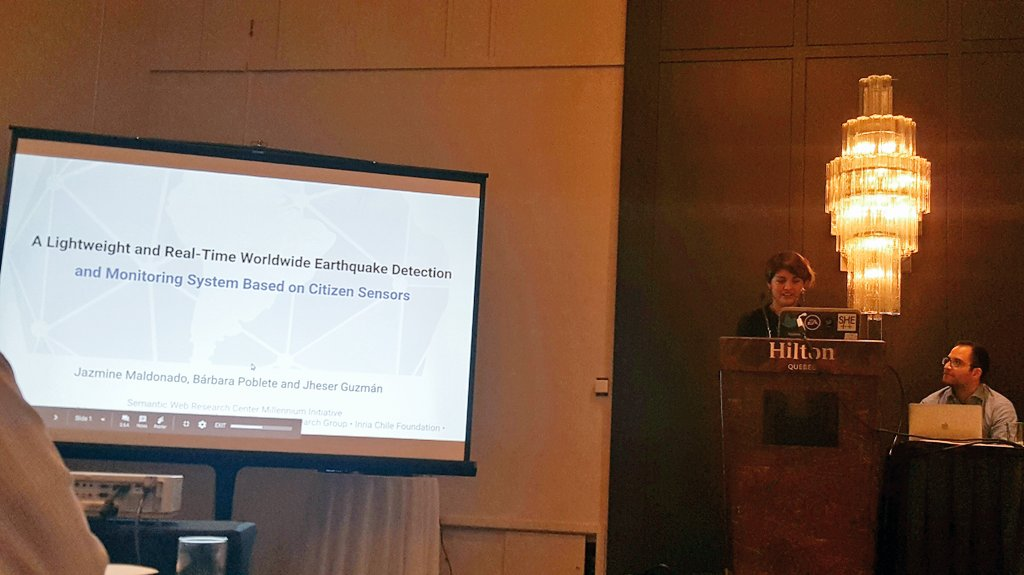
\includegraphics[width=0.5\textwidth]{imagenes/hcomp.jpg}
	\caption{Jazmine Maldonado presentando en HCOMP 2017.}
\label{fig:hcomp}
\end{figure} 

El artículo publicado se adjunta en la siguiente página. 

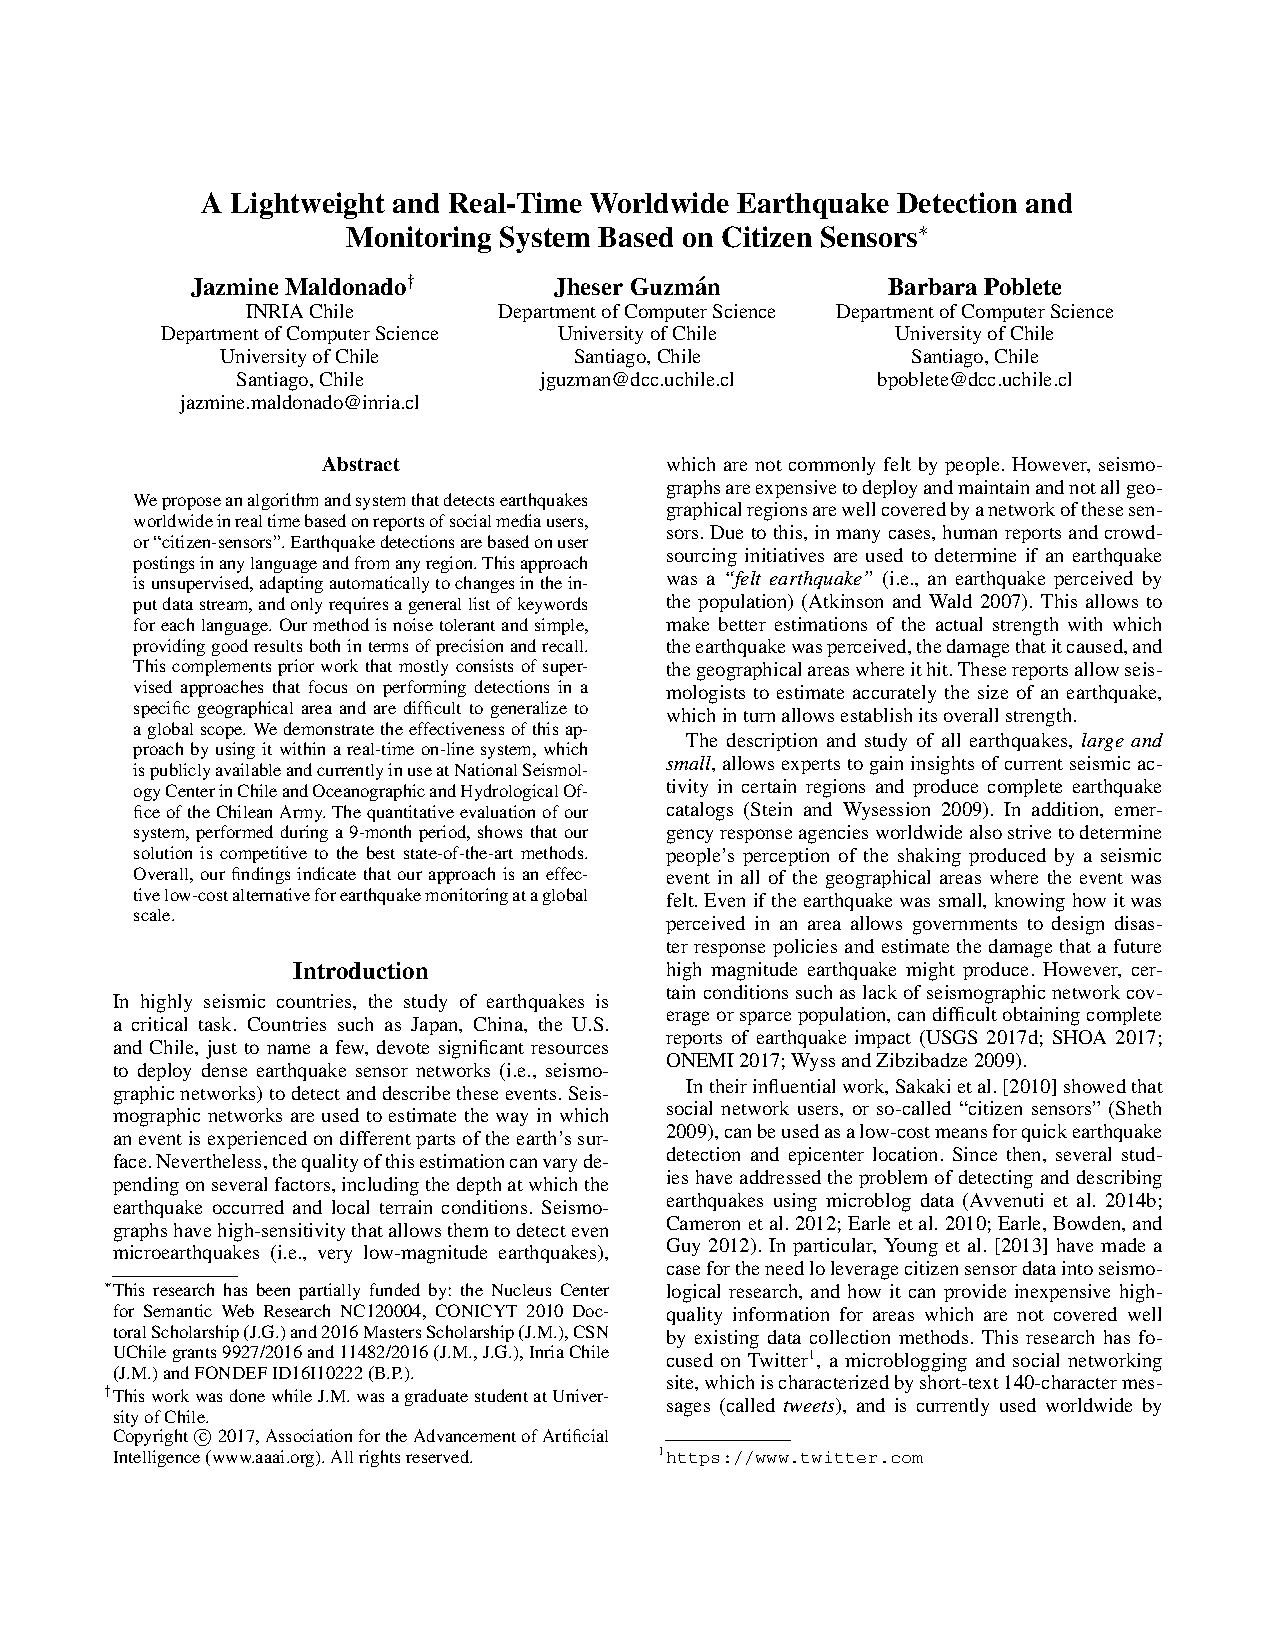
\includepdf[pages={1-10},scale=1]{documentos/paper_earthquake.pdf} % paper HCOMP 2017

\phantomsection
\addcontentsline{toc}{chapter}{Anexo C: Menciones en la prensa}
\chapter*{Anexo III: Menciones en la prensa}
\label{anexo:prensa}

\begin{itemize}
\item Noticia en publimetro el 23 de Marzo del 2016. \\
{\tiny \url{https://www.publimetro.cl/cl/noticias/2016/03/23/chilenos-disenan-plataforma-que-usara-twitter-localizar-epicentro-sismos.html}}
\item Entrevista a Bárbara Poblete en CNN Chile el 27 de Marzo del 2016.\\ 
{\tiny \url{http://www.cnnchile.com/noticia/2016/03/27/plataforma-busca-medir-los-sismos-a-traves-de-twitter-en-chile}}
\item Noticia en Emol el 23 de Marzo del 2016.\\
{\tiny \url{http://www.emol.com/noticias/Tecnologia/2016/03/23/794547/Usuarios-como-reporteros-Twitter-ayudara-a-detectar-y-localizar-sismos.html}}
\item Mención de la aplicación Web en una nota de prensa de la Red de Televisión Global China el 14 de Agosto del 2016.\\
{\tiny \url{https://america.cgtn.com/2016/08/14/chile-leading-the-way-to-decrease-earthquake-devastation}}
\item Noticia en El Comercio (periódico de Perú) el 24 de Marzo del 2016.\\
{\tiny \url{https://elcomercio.pe/tecnologia/actualidad/twitter-ayudara-detectar-localizar-sismos-chile-394051}}
\item Mención de Twicalli en una noticia sobre Big Data en El Mostrador el 10 de Mayo del 2017.\\
{\tiny \url{http://www.elmostrador.cl/cultura/2017/05/10/big-data-o-cuando-la-tecnologia-ya-no-dio-abasto-para-procesar-la-produccion-de-informacion}}
\end{itemize} % menciones en la prensa
%\chapter*{Anexo IV: Base de Datos}
\label{anexo:bd} % especificación de la base de datos

\end{document}
